%% 
%% This is a sample doctoral dissertation.  It shows the appropriate
%% structure for your dissertation.  It should handle most of the
%% strange requirements imposed by the Grad school; like the different
%% handling of titles of one/many appendices.  It will automatically
%% handle the linespacing changes.  The body default is double-spaced
%% (except when you use the singlespace or condensed options).  The
%% default for quotations is single-space, and the default for tabularmultithreaded programs
%% environments is also single-space.  
%%
%% This class adds the following commands and environments to the
%% report class, upon which it is based:
%% Commands
%% ------------
%% \degree{name}{abbrv} -- Sets the name and abbreviation for the degree.
%%                         These default to ``Doctor of Philosopy''
%%                         and ``Ph.D.'', respectively.
%% \copyrightyear{year} -- for the copyright page.
%% \bachelors{degree}{institution} -- for the abstract
%% \masters{degree}{institution}   --  "
%%     if you have other degrees you may use
%% \secondbachelors{degree}{institution}
%% \thirdbachelors{degree}{institution}
%% \secondmasters{degree}{institution}
%% \thirdmasters{degree}{institution}
%% \priordoctorate{degree}{institution}
%%
%% \committeechair{name}           -- for the signature page
%% or, if you have two co-chairs:
%% \cochairs{first name}{second name}
%%
%% \firstreader{name}              --  "
%% \secondreader{name}             --  "
%% \thirdreader{name}              -- (optional)
%% \fourthreader{name}             --  "
%% \fifthreader{name}              --  "
%% \sixthreader{name}              --  "
%% \departmentchair{name}          -- for the signature page
%% \departmentname{name}           --  "
%%
%% \copyrightpage                  -- produces the copyright page
%% \signaturepage                  -- produces the signature page
%%
%% \frontmatter                    -- these are required in their various
%% \mainmatter                     -- appropriate locations
%% \backmatter                     --
%%
%% \unnumberedchapter[toc]{name}   -- like \chapter, except that it
%%                                    produces an unnumbered chapter;
%%                                    alternatively, like \chapter*,
%%                                    except that it lists the chapter
%%                                    in the table of contents.
%%
%% New environments:
%%   dedication  -- for the dedication
%%   abstract    -- for the abstract
%%
%% The thesis documentclass is built on top of the report document class.
%% It accepts all of the options that the report class accepts, plus the
%% following:
%%     doublespace -- the default, indicates double spacing as per U.Mass.
%%                    requirements.  You will need this when you do your
%%                    final copy.
%%     singlespace -- for earlier work, not acceptable to the Grad school
%%     condensed   -- for earlier work, not acceptable to the Grad school,
%%                    creates condensed versions of the frontmatter. 
%%                    Condensed implies singlespace.
%%     dissertation - the default, indicates that this document is a
%%                    dissertation.
%%     proposal    -- indicates that this document is a dissertation proposal,
%%                    rather than a dissertation.  This will only change the
%%                    wording on the title and signature pages.
%%     thesis      -- indicates that this document is a Master's thesis 
%%                    rather than a doctoral dissertation.  This also changes
%%                    the default for \degree to Master of Science, M.S.
%%     allowlisthypenation -- (the default), allows hyphenation of words in
%%                    the table of contents, the list of figures, and the list
%%                    of tables.  I believe that this is acceptable to the 
%%                    Graduate School.
%%     nolisthyphenation -- disallows hyphenation of words in the table of
%%                    contents and the list of figures and tables.  Use this 
%%                    option if the Grad School doesn't like your hyphenation.
%%     nicerdraft  -- relaxes some of the Grad School's rules for working with
%%                    drafts -- has no effect when doublespace is in effect
%%     nonicerdraft -- the default, leaves things in draft as they will be in
%%                     the final version
%% umthesis changes the default font size to 12pt, but you may specify 10pt or
%%   11pt in the options.
%%\documentclass[proposal]{umthesis}          % for Ph.D. dissertation or proposal
\documentclass{umthesis}          % for Ph.D. dissertation or proposal
%\documentclass{umthesis}          % for Ph.D. dissertation or proposal
% \documentclass[thesis]{umthesis}  % for Master's thesis

\usepackage{color}
\usepackage{listings}
\usepackage{amsmath}
\usepackage{amsfonts}
\usepackage{amssymb}
\usepackage{comment}
\usepackage{graphicx, subfigure}
\usepackage{url}
\usepackage{pifont}% http://ctan.org/pkg/pifont
\usepackage{tabularx}

%\lstset{ %
% language=C,                    % choose the language of the code
% basicstyle=\footnotesize,       % the size of the fonts that are used for the code
%numbers=left,                   % where to put the line-numbers
%numberstyle=\footnotesize,      % the size of the fonts that are used for the line-numbers
%stepnumber=1,                   % the step between two line-numbers. If it is 1 each line will be numbered
%numbersep=5pt,                  % how far the line-numbers are from the code
%backgroundcolor=\color{white},  % choose the background color. You must add \usepackage{color}
%showspaces=false,               % show spaces adding particular underscores
%showstringspaces=false,         % underline spaces within strings
%showtabs=false,                 % show tabs within strings adding particular underscores
%frame=single,           % adds a frame around the code
%tabsize=2,          % sets default tabsize to 2 spaces
%captionpos=b,           % sets the caption-position to bottom
%breaklines=true,        % sets automatic line breaking
%breakatwhitespace=false    % sets if automatic breaks should only happen at whitespace
%escapeinside={\%*}{*)}          % if you want to add a comment within your code
%}

%%
%% If you have enough figures or tables that you run out of space for their
%% numbers in the List of Tables or List of figures, you can use the following
%% command to adjust the space left for numbers.  The default is shown:
%%
%% \setlength{\tablenumberwidth}{2.3em}
\newcommand{\dthreads}{{\scshape Dthreads}}
\newcommand{\Dthreads}{{\scshape Dthreads}}
\newcommand{\Grace}{{\scshape Grace}}
\newcommand{\grace}{{\scshape Grace}}
\newcommand{\Sheriff}{{\scshape Sheriff}}
\newcommand{\sheriff}{{\scshape Sheriff}}
\newcommand{\SheriffProtect}{\textsc{Sheriff-Protect}}
\newcommand{\sheriffProtect}{\textsc{Sheriff-Protect}}
\newcommand{\sheriffprotect}{\textsc{Sheriff-Protect}}
\newcommand{\SheriffDetect}{\textsc{Sheriff-Detect}}
\newcommand{\sheriffDetect}{\textsc{Sheriff-Detect}}
\newcommand{\sheriffdetect}{\textsc{Sheriff-Detect}}
\newcommand{\Predator}{\textsc{Predator}}
\newcommand{\predator}{\textsc{Predator}}
\newcommand{\DoubleTake}{\textsc{DoubleTake}}
\newcommand{\doubletake}{\textsc{DoubleTake}}
\newcommand{\pthreads}{\texttt{pthreads}}
\newcommand{\cmark}{\ding{52}} %51 or 52
\newcommand{\xmark}{\ding{53}}% 53, 54, 55, 56
\newcommand{\CC}[1]{{\large \textbf{\color{red}CC:} \emph{#1} \newline}}
\lstdefinestyle{tt}{basicstyle=\small\ttfamily,keywordstyle=\bfseries,language=C, numbers=left, firstline=1}
%numberblanklines=false
\lstdefinestyle{rm}{basicstyle=\ttfamily,keywordstyle=\slshape,language=[LaTeX]{TeX}}


\begin{document}

%%
%% You must fill in all of these appropriately
\title{Reliable and Efficient Multithreading}
\author{Tongping Liu}
\date{May 2014} % The date you'll actually graduate -- must be
                     % February, May, or September
\copyrightyear{2014}
\bachelors{B.S.}{Harbin Institute of Technology}
\masters{M.E.}{Huazhong University of Science and Technology}
\secondmasters{M.S.}{UNIVERSITY OF MASSACHUSETTS AMHERST}
\committeechair{Emery D. Berger}
\firstreader{Scott F. H. Kaplan}
\secondreader{Yuriy Brun}
\thirdreader{Israel Koren}   % Optional
%\fifthreader{}            % Optional
%\sixthreader{}            % Optional
\departmentchair{Lori A. Clarke}
\departmentname{School of Computer Science}

%% If your degree is something other than a Ph.D. (for a dissertation), or
%% an M.S. (for a thesis), you will need to uncomment the appropriate
%% following line:
%%
%% \degree{Doctor of Education}{Ed.D.}
%% \degree{Doctor of Philosophy}{Ph.D.}
%%
%% \degree{Master of Arts}{M.A.}
%% \degree{Master of Arts in Teaching}{M.A.T.}
%% \degree{Master of Business Administration}{M.B.A.}
%% \degree{Master of Education}{M.Ed.}
%% \degree{Master of Fine Arts}{M.F.A.}
%% \degree{Master of Landscape Architecture}{M.L.A.}
%% \degree{Master of Music}{M.M.}
%% \degree{Master of Public Administration}{M.P.A.}
%%\degree{Master of Public Health}{M.P.H.}
%% \degree{Master of Regional Planning}{M.R.P.}
%% \degree{Master of Science}{M.S.}
%% \degree{Master of Science in Accounting}{M.S. Acctg.}
%% \degree{Master of Science in Chemical Engineering}{M.S. Ch.E.}
%% \degree{Master of Science in Civil Engineering}{M.S.C.E.}
%% \degree{Master of Science in Electrical and Computer Engineering}{M.S.E.C.E.}
%% \degree{Master of Science in Engineering Management}{M.S. Eng. Mgt.}
%% \degree{Master of Science in Environmental Engineering}{M.S. Env. E.}
%% \degree{Master of Science in Industrial Engineering and Operations Research}{M.S.I.E.O.R.}
%% \degree{Master of Science in Manufacturing Engineering}{M.S. Mfg. Eng.}
%% \degree{Master of Science in Mechanical Engineering}{M.S.M.E.}
%%
%% \degree{Professional Master of Business Administration}{P.M.B.A.}


%%
%% These lines produce the title, copyright, and signature pages.
%% They are Mandatory; except that you could leave out the copyright page
%% if you were preparing an M.S. thesis instead of a PhD dissertation.
\frontmatter
\maketitle
\copyrightpage     %% not required for an M.S. thesis
\signaturepage

%%
%% Dedication is optional -- but this is how you create it
%\begin{dedication}              % Dedication page
%  \begin{center}
%   \emph{ XXXXXX }       
%  \end{center}
%\end{dedication}

%%
%% Epigraph goes here...(aka frontispiece)
%% \chapter{Epigraph}?????

%%
%% Acknowledgements are optional...yeah, right.
\chapter{Acknowledgments}             % Acknowledgements page
%  Thanks to all those fine shepherds. Not to mention all the great
%  border collies and suchlike fine animals.

%%
%% Abstract is MANDATORY. -- Except for MS theses
I would first thank Emery Berger, my Ph.D. thesis advisor, for his wonderful supervision and enthusiastic support in the development of this thesis work. Emery taught me to work on those important and practical projects, and take everything seriously. I hope that I could be as lively, enthusiastic, and energetic as Emery one day to my students. I also thank my dissertation committee: Scott Kaplan, Yuriy Brun, and Israel Koren, for their valuable insights, feedback, and support. 

I am also fortunate to work with Chen Tian, Timothy Richards, Prashant Shenoy, Ziang Hu, Daniel Waddington, Seetharami Seelam, Wei Tan, Liana Fong, and Arun Iyengar. They provided me valuable guidance and suggestions on those projects we worked on together. I also thank Leeanne Leclerc, James Allan, and Laurie Downey for their help to make my experience at UMASS go as smoothly as possible. 

I couldn't finish my thesis without the help of PLASMA  labmates, including Charlie Curtsinger, Ting Yang, Gene Nowark, Kaituo Li, John Altidor, Divya Krishnan, Dan Barowy, Dimitar Gochev, John Vilk, Nitin Gupta, Jacob Evans, Justin Aquadro, and Emma Tosch. I also feel lucky to meet many friends in the computer science department, including Rui Wang, Ming Li, Tingxin Yan, Zongfang Lin, Kun Tu, Xiaojian Wu, Pengyu Zhang, Bo Jiang, Xiaozhen Tie, Fangyuan Zhou, Hong Zhang, Yue Wang, Wenzhao Liu, etc. I will never forget your help in my life. 

Finally, I would give my special thanks for my wife, Yuyu Tang. She quit her job to support my crazy idea of getting a Ph.D. degree. She also took care of most of the household duties and spent much of her time taking care of our two adorable kids, Yanbin Liu (Grace) and Yanlin Liu (Eileen). My buddy, Guangming Zeng, also deserves my special thanks for his generous help and valuable discussion when I chose the career in the computer science field. I also want to thank my kids, my late grandma, my parents, sisters, and brothers for their understanding and support.    



\begin{abstract}                % Abstract
The advent of multicore architecture has increased the demand for multithreaded programs. It is notoriously far more challenging to write parallel programs correctly and efficiently than sequential ones, because of the wide range of concurrency errors and performance problems. 

In this thesis, I developed a series of runtime systems and tools to combat concurrency errors and performance problems of multithreaded programs.

The first system, \dthreads{}, automatically ensures determinism for unmodified C/C++ applications using the \pthreads{} library, without requiring programmer intervention and hardware support. Because of determinism, it greatly simplifies the understanding and debugging of multithreaded programs. \dthreads{} outperforms the previous state-of-the-art (CoreDet) more than $3\times$, thus greatly propelling the progress of this field. \dthreads{} leverages the isolated executions, combined with a deterministic commit protocol and a deterministic memory allocator, to ensure robust deterministic execution with very low runtime overhead.

The second system attacks one of the notorious performance problems of multithreaded programs, false sharing. We provide the first accurate and precise detection tool, \sheriffdetect{}, which can pinpoint the name of global variables or the line of source code of heap objects that have false sharing problems inside, without any false positives. We also provide a runtime system, \SheriffProtect{}, to automatically boost the performance of those programs with false sharing problems inside, when fixing false sharing problems is unable to improve the performance or is impossible because of lacking source code or time. 

The third system, \predator{}, improves the effectiveness of false sharing detection. It can detect one more type of false sharing, read-write false sharing, and work on applications without any limitations. Also, it can even detect false sharing problems without occurrences, thus overcomes a shortcoming of all existing tools: they can only detect those observed false sharing problems. \Predator{} is also the first tool to precisely detect false sharing problems happening in those complex real applications. 

\end{abstract}

%%
%% Preface goes here...would be just like Acknowledgements -- optional
%% \chapter{Preface} 
%% ...


%%
%% Table of contents is mandatory, lists of tables and figures are 
%% mandatory if you have any tables or figures; must be in this order.
\tableofcontents                % Table of contents
%\listoftables                   % List of Tables
\listoffigures                  % List of Figures

%%
%% We don't handle List of Abbreviations
%% We don't handle Glossary

%%%%%%%%%%%%%%%%%%%%%%%%%%%%%%%%%%%%%%%%%%%%%%%%%%%%%%%%%%%%%%%%%%%%%%%%%
%% Time for the body of the dissertation
\mainmatter   %% <-- This line is mandatory

%%
%% If you want an introduction, which is not a numbered chapter, insert
%% the following two lines.  This is OPTIONAL:
\unnumberedchapter{Introduction}
For decades, applications enjoyed automatic and regular performance gains from increasingly faster CPU speed.  However, this trend has stopped permanently because of hard physical limits. Increasing CPU speed results in consuming more energy and generating more heat. Intel and other vendors have turned to providing more and more cores on a single machine, which brings us the multi-core era. The appearance of multi-core drives the biggest revolution multithreaded programs of software development: software has to be programmed in a concurrent and parallel way in order to exploit the benefits of multi-core machines.

Building efficient and reliable concurrent software is still a challenging task because of the following reasons. First, concurrency requires programmers to think in an unnatural way that humans find difficult.  Second, existing languages and tools are inadequate to detect or prevent concurrency errors and performance anomalies. 

% Why we need determinism? Concurrency errors?
Concurrency errors of multithreaded programs, such as race conditions, atomicity violations, order violations and deadlocks, are very hard to debug ~\cite{Lu:2008:LMC:1346281.1346323}, because their occurrences highly depend on some specific conditions, such as thread interleavings and CPU scheduling ~\cite{DBLP:conf/icse/BallBHMQ09,DBLP:conf/asplos/BurckhardtKMN10}. Instead of detecting possible concurrency errors, one promising alternative approach is to attack the problem of concurrency bugs by eliminating its source: non-determinism. A fully \emph{deterministic multithreading system} would prevent Heisenbugs by ensuring that executions of the same program with the same inputs always yield the same results, even in the face of race conditions in the code. Such a system would not only dramatically simplify debugging of concurrent
programs~\cite{Carver:1991:RTC:624586.625040} and reduce their attendant testing overhead, but would also enable a number of other applications. For example, a deterministic multithreaded system would greatly simplify record-and-replay for multithreaded programs~\cite{Choi:1998:DRJ:281035.281041,LeBlanc:1987:DPP:32387.32396} and the deterministic replication of a multithreaded application on different machines for fault tolerance~\cite{deterministic-process-groups,1134000,224058,replicant-hotos}.

% Why we need to find out false sharing problems.
Besides concurrency errors, writing efficient multithreaded programs remains challenging too. False sharing problem is one of the notorious performance problems inside multithreaded programs~\cite{falseshare:Analysis, falseshare:effect}. It occurs when multiple threads, running on different cores with their separate caches, are accessing logically independent words in the same cache line. If a thread modifies anything inside a cache line, cache coherence protocol invalidates the duplicates of this cache line in other caches in order to guarantee correctness of programs, which is crucial for true sharing cases. However, it is totally unnecessary for false sharing cases. False sharing can force one core to wait unnecessarily for updates from another processor, thus wasting both the CPU time and precious memory bandwidth in the same time. 

\subsection*{Contributions}

This thesis handles two categories of problems inside multithreaded programs, the reliability problem and the performance problem, and makes the following contributions:

\begin{itemize}
\item \Sheriff{} framework: I developed a novel processes-as-threads framework by borrowing the idea from Grace~\cite{grace}. \sheriff{} is a software-only drop-in replacement of the stand \pthreads{} library. It turns threads into processes, with separate address spaces but the shared file table. \sheriff{} provides per-thread memory protection and isolation on page granularity, relying on the stand memory protection mechanism and twining-and-diffing mechanism. \sheriff{} enables a range of possible applications, including language support and enforcement of data sharing, software transactional memory, thread-level speculation, and race detection. 

\item I developed an efficient deterministic multithreading system, \dthreads{}, for unmodified C/C++ applications,  without programmer intervention and hardware support. \dthreads{} is based on the \sheriff{} framework to isolate executions of different threads. \dthreads{} outperforms the previous state-of-the-art runtime system (CoreDet) by a factor of 3, and often matches and sometimes exceeds the performance with the standard \pthreads{} library. \Dthreads{} enforces robust/stable determinism even in the face of data races, greatly simplifying program understanding and debugging: programs always behave the same, even with different inputs and on different hardware, as long as the synchronization order is staying the same. Because of this, \dthreads{} can also be used to support replicated executions of multithreaded applications for fault tolerance purposes.

\item 
Based on the \sheriff{} framework, I developed another two tools, \SheriffDetect{} and \SheriffProtect{}, to deal with false sharing problems of multithreaded programs, one of the notorious performance problems. 
\SheriffDetect{} find instances of false sharing accurately (no false positives), runs with low overhead (on average 20\%), and can precisely pinpoint the exact objects involved in false sharing. \SheriffProtect{} mitigates false sharing problems by adaptively isolating shared accesses on a cache line from different threads into separate physical addresses, effectively eliminating the performance impact of false sharing. It can boost the performance automatically for those multithreaded applications with false sharing problems inside, without the need of programmer intervention. 

\item I also developed a tool, \predator{}, to improve the effectiveness of false sharing detection. Instead of relying on the \sheriff{} framework to track memory writes, \predator{} employs compiler instrumentation to track read and write memory accesses, which make it possible to detect one more type of false sharing, read-write false sharing. \Predator{} also overcomes a key limitation of previous detection tools: existing tools can only detect those observed false sharing problems. However, the occurrences of false sharing highly depend on memory layout and size of a cache line, which are affected by a lot of dynamic properties. \Predator{} can predict potential false sharing that does not manifest in a given execution but may appear---and greatly degrade application performance—--in a slightly different execution environment. \Predator{} is the first false sharing tool able to automatically and precisely uncover false sharing problems in real applications, including MySQL and the Boost library.


\end{itemize}

\subsection*{Outline}
The rest of this thesis is organized as follows. Chapter~\ref{chapter:problems} describes the reliability and performance problems of multithreaded programs, which we are going to handle in this thesis. Chapter~\ref{sec:sheriffframework} describes the processes-as-threads framework, \sheriff{}, which is the basis for \dthreads{}, \SheriffDetect{} and \SheriffProtect{}. Chapter~\ref{chapter:dthreads} describes \dthreads{} that ensures deterministic execution for multithreaded programs linking to this drop-in library. Chapter~\ref{chapter:sherifftools} discusses how to precisely detect and automatically tolerate false sharing problems based on the \sheriff{} framework. Chapter~\ref{chapter:preditor} describes a generalized false sharing detection tool by combining compiler instrumentation and runtime system, which improves the effectiveness of false sharing detection. 
Chapter~\ref{chapter:relatedwork} provides a substantial comparison between previous work and our approaches and Chapter~\ref{chapter:conclusion} concludes the thesis with its contributions and possible future work. 


%%
%% Some sample text



\chapter{Problems of multithreaded programs}
\label{chapter:problems}

Writing Multithreaded programs can encounter concurrency errors and performance anomalies. This thesis discusses in detail two different types of problems, non-determinism and false sharing.  We discuss the definitions, causes of these problems and their possible consequence as follows.

\section{Non-determinism}
\label{sec:nondeterminism}

\subsection{Background}
Deterministic behavior of programs is the most desirable behavior: given the same input, a program
produces the same output and generates the same execution. Relying on this behavior, it is able to figure out problems of programs. 

In reality, it is relatively easy for sequential programs to achieve this target if a program do not explicitly rely on a randomized mechanism. 
However, it is hard to do this for parallel programs. In shared memory multithreaded programs, an application can only experience one of many possible 
schedules at a time. Thread scheduling, the order of memory accesses on the shared data, operations depending on timing and non-deterministic synchronizations, can easily lead to different executions of the same program.


\begin{figure*}[!ht]
{\centering
\fbox{
\subfigure{\lstinputlisting[numbers=none,frame=none,boxpos=t]{fig/nondeter.sample1}}
\hspace{20pt}
\subfigure{\lstinputlisting[numbers=none,frame=none,boxpos=t]{fig/nondeter.sample2}}
\hspace{20pt}
\subfigure{\lstinputlisting[numbers=none,frame=none,boxpos=t]{fig/nondeter.sample3}}
}
\caption{Non-determinism problem 
\label{fig:nondeterminism}}
}
\end{figure*}

A simple example of non-deterministic execution can be seen in Figure~\ref{fig:nondeterminism}. When using the standard \pthreads{} library, this program can print ``1,0'', ``0,1'' or ``1,1'' in the end, depending on the order of memory accesses from different threads. We actually run this simple program for one million times. About 99.43\% of time, it will print ``1,0'', while 0.56\% it will print ``0,1'' and 0.01\% it will print ``1,1''. According to the semantics of this program, both ``1,0'' and ``1,0'' are correct results. Thus, the unexpected result (``1,1'') caused by race conditions happens very rarely, only about 0.01\%.  
It is very difficult to observe/reproduce these rare cases that caused by race conditions.

\subsection{Source of Non-determinism}
Non-determinism can be caused by a lot of sources, both external sources and internal sources. For example, the timing of external inputs is one of the sources that can lead to non-determinism. This section only lists internal sources of non-determnism~\cite{costofdeterminism}. 
 
\emph{Thread Communication}: 
Thread communication is the most important source of non-determinism for multithreaded programs. 
First, the order of accesses on shared variables may change from one execution to the other. Second, the orders on shared resources, such as memory allocation, synchronization, and library/system calls, vary across different executions. 
Third, the interaction between compiler and run-time can be changed. For example, lazy binding may cause the thread that  performs address resolution to execute much more instructions than others. 

\emph{Memory Layout}: 
Address space layout randomization (ASLR) in Linux environment brings non-deterministic memory addresses of instructions and data across different executions. Thus, a program relying on memory addresses lead to non-deterministic execution of a program. 

\emph{System or Library Dependence}:
Some library or system calls cannot return deterministic results. For example, the \texttt{gettimeofday()} library call returns different time values at different time, and \texttt{read} system calls may return different number of bytes, depending on the timing of issuing \texttt{read} calls.  An application relying on them can execute non-deterministically too. 


\subsection{Effect of Non-determinism}
Because of different sources of non-determinism, listed in the above section, existing multithreaded applications can not run deterministically: given the same input, a program can have different executions that may or may not lead to different outputs. 

Non-determinism can greatly complicate the reasoning and debugging in development phases, which makes it hard for programmers to reproduce program errors. 
Even worse, since executions of deployment can vary from executions of development phase, a lot of programmer errors can be easily leaked to customers.

By contrast, determinism greatly simplifies the understanding and debugging of multithreaded programs. We can always guarantee the same executions on both development phases and the deployment phases, thus there is no need to worry about erroneous results. 

\section{False Sharing}
\label{sec:falsesharingproblems}

\subsection{Definition}
% What is the definition of false sharing?
False sharing occurs when different processors in a shared-memory parallel system are referencing distinct fields within the same coherence block (page or cache line) simultaneously, thereby inducing ``unnecessary'' coherence traffic~\cite{Bolosky:1993:FSE:1295480.1295483}. 

Although it is difficult or impossible to know where a thread runs in an actual execution, we can conservatively assume that different threads are running on different processors with separate cache. Thus, in the multithreaded environment, false sharing simply implies: multiple threads access distinct parts of the same cache line simultaneously, while one of them is a write operation. False sharing is shown in Figure~\ref{fig:fs}. 
Based on the relationship of false sharing objects, 
false sharing can be classified into inter-object and intra-object false sharing. When two different objects in the same cache line are accessed by different threads simultaneously, that is inter-object false sharing. Otherwise, it is intra-object false sharing. 

There is another concept, true sharing, which is opposite of false sharing. In true sharing (Figure~\ref{fig:ts}), multiple threads are accessing the same word. 

There is another way to differentiate false sharing with true sharing. False sharing is avoidable, while true sharing is not. 

\begin{figure*}
\begin{center} 
\subfigure[False sharing]{%
   \label{fig:fs}
   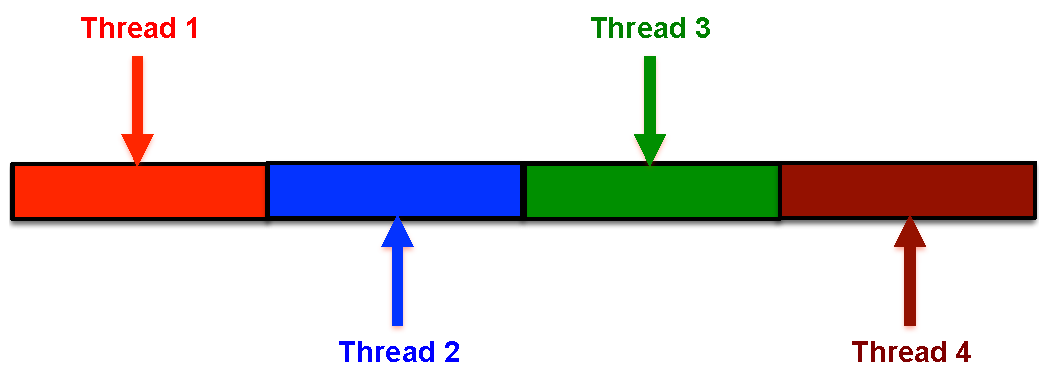
\includegraphics[width=2.4in]{sheriff/figure/falsesharing.pdf}
}%
\hspace{50pt}
\subfigure[True sharing]{%
   \label{fig:ts}
   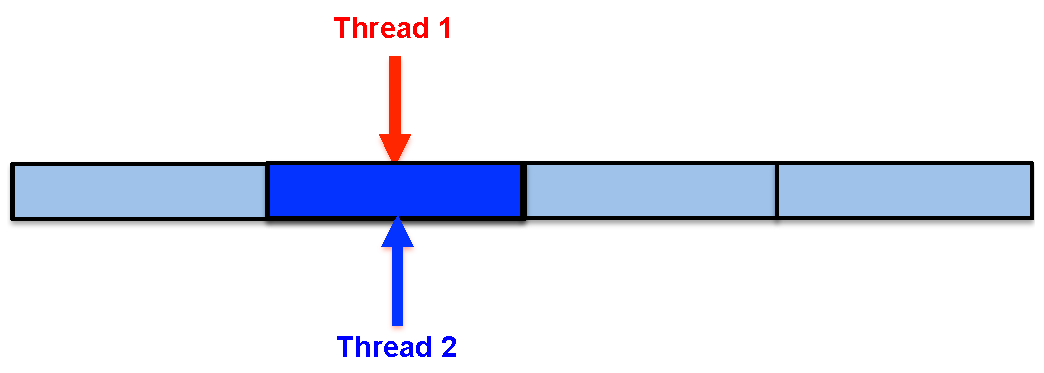
\includegraphics[width=2.4in]{sheriff/figure/truesharing.pdf}
}%
\end{center}
%\includegraphics{fig/potential.pdf}
\caption{False sharing and true sharing in a cache line with four words. }
\label{fig:fsexample}
\end{figure*}

% The classification of false sharing?

\subsection{Reason of False Sharing}

As shown in Figure~\ref{fig:fsexample}, false sharing only occurs when the size of coherence block is larger than that of a single word. Multiple processors may reference different words of the same coherence block. In this perspective, a single-word block size can avoid false sharing problems. 

However, using a single-word block size is not the actual case. In reality, the size of a coherence block (cache line) is normally 32 or 64 bytes. The reason of using multiple words in a cache line is to reduce the groups of transfers between the main memory and the cache since programs always have some spatial locality of reference. Those adjacent words are very likely to be referenced in the future.

From the performance perspective, reducing the coherence block size to one word may minimize the data to transferred, but can increase the number of transfers. Thus, the overhead of transferring less data at a time can be larger than the benefit of eliminating false sharing coherence traffic. Actually, the hardware trend of cache line is to increase the size of cache line, which makes false sharing problems increasingly common. 

\subsection{Performance Impact}
\label{falsesharing}
False sharing can greatly slowdown the execution of multithreaded programs, which depends on many factors, including the cache block size, data layout, program access patterns, and the cost of coherence operations~\cite{Bolosky:1993:FSE:1295480.1295483}. 

In a typical shared-memory system, each processor may have a separate cache. In order to increase the access speed, when a processor references a word, all the data inside the same cache line is fetched from the main memory to its corresponding cache. 
When multiple processors are accessing distinct words of the same cache line simultaneously, the shared data can be replicated into caches of different processors that access this cache line. Thus, it is very important to maintain the coherence across different processors: if any copy is changed, this change should be propagated to other processors immediately for correctness purposes. In real hardware, this data propagation only happens lazily when the data is accessed again, thus duplicates are invalidated at first. When a processor access an invalidated cache line, it should wait for the data propagating from other processors, wasting CPU time and memory bandwidth simultaneously. 

In the false sharing case, this propagation is totally unnecessary because different threads are actually accessing different parts of the same cache line. Thus, there is no need for a processor to get the updated data that is not going to access. However, hardware can only tracks the change of data on the granularity of a cache line and have to propagate those changes if any word has been changed. When there are interleaved writes, issued by different processors, on the same cache line, the ping-pong effect of loading-and-invalidating of data on this cache line can greatly slow the execution of programs. 
Programs with false sharing can even run slower in a multi-core machine than in a single-core machine, losing the benefit of multiple cores.  

Many common programming practices can easily cause false sharing. For example, different threads accessing different entries of the same global array, listed in Figure~\ref{fig:falsesharingexample}, is such an example. This example has no correctness problem, but a serious performance problem. 

\begin{figure*}[!ht]
{\centering
\fbox{
\subfigure{\lstinputlisting[numbers=none,frame=none,boxpos=t]{fig/falsesharing.sample1}}
\hspace{20pt}
\subfigure{\lstinputlisting[numbers=none,frame=none,boxpos=t]{fig/falsesharing.sample2}}
}
\caption{False sharing problem
\label{fig:falsesharingexample}}
}
\end{figure*}

We actually run this program on a real machine with 8 cores and Figure~\ref{fig:fsperfimpact} presents performance results. On this evaluation, we specifically choose a different number of threads, matching the number of hardware cores, from 1 thread to 8 threads, to perform the same amount of workload. We find out that false sharing can greatly impact the performance, which brings around $13\times$ difference between actual performance and the expected performance. Two trends--the prevalence of multicore architectures and
the expected increase in the number of multithreaded applications in broad use, and increasing cache line sizes--are likely to make false sharing increasingly common.

\begin{figure*}[!t]
\centering
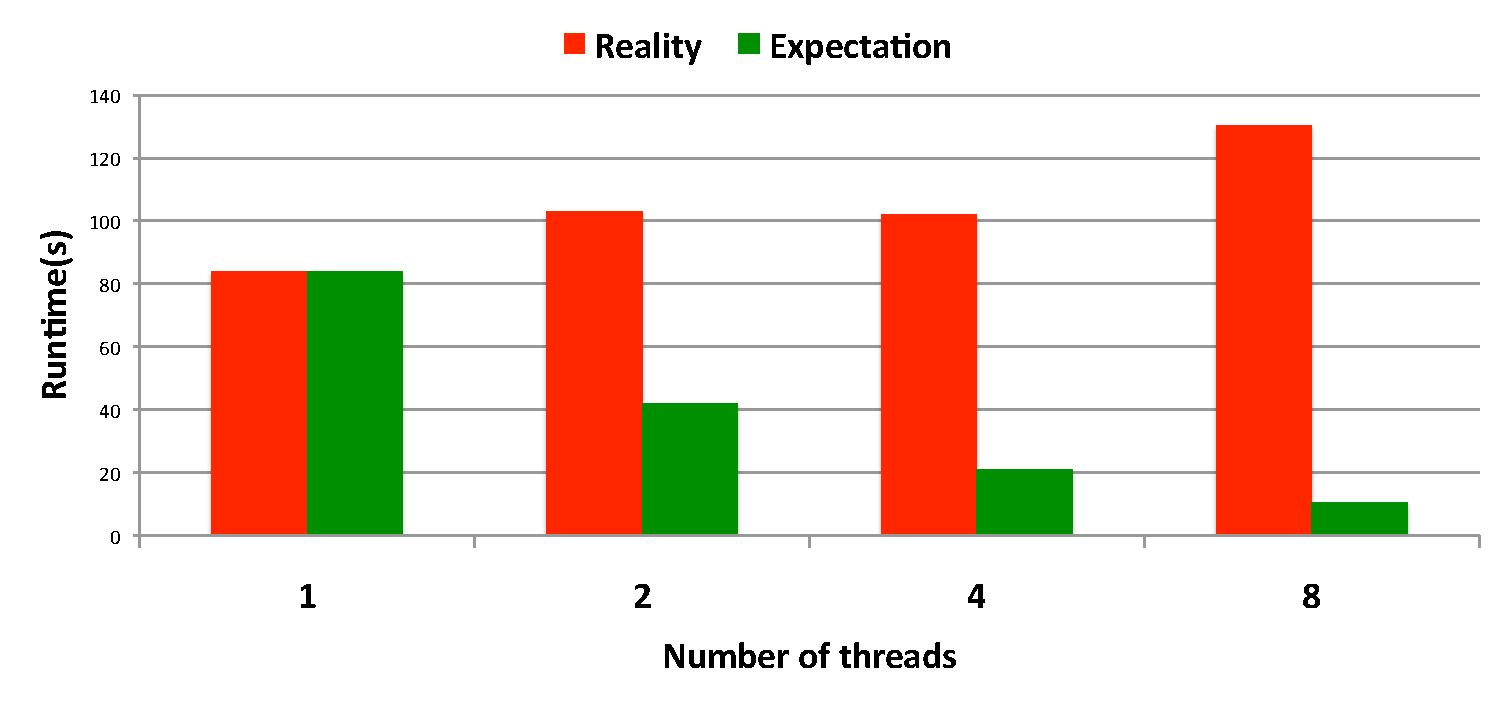
\includegraphics[width=6in]{fig/fsperfimpact.pdf}
\caption{
False sharing performance impact for the simple program shown in Figure~\ref{fig:falsesharingexample}.
\label{fig:fsperfimpact}
}
\end{figure*}

\subsection{Fixing False Sharing}
There are several ways to fix false sharing problems after they are identified. The basic idea is to prevent multiple threads from accessing the same cache line simultaneously.  

The first way is to change the size of corresponding structure or class, by padding some useless words. Thus, we can prevent two threads concurrently accessing the same cache line. One example of prevention, linear\_regression, can be seen in Section~\ref{sec:effecteval}.

The second way is to assign the value to thread-local variables at first. Then different threads only update their own local variables, and commit those changes back to the shared variable in the end. For example, the problem shown in Figure~\ref{fig:falsesharingexample} is fixed using this method, see Figure~\ref{fig:falsesharingexamplefix}. 

\begin{figure*}[!ht]
{\centering
\fbox{
\subfigure{\lstinputlisting[numbers=none,frame=none,boxpos=t]{fig/falsesharing.sample2fix}}
}
\caption{Fixing the false sharing problem shown in Figure~\ref{fig:falsesharingexample}.
\label{fig:falsesharingexamplefix}}
}
\end{figure*}

Some other approaches, to fix false sharing problems automatically, is described in detail in Section~\ref{sec:fspreventwork}, but they all suffer different shortcomings. 







%\chapter{\DoubleTake{}: Evidence-Based Dynamic Analysis}
%
Dynamic analysis tools are widely used to find bugs in applications. They are popular among programmers because of their precision---for many analyses, they report no false positives---and can pinpoint the exact location of errors, down to the individual line of code.

Perhaps the most prominent and widely used dynamic analysis tool for C/C++ applications is Valgrind~\cite{Valgrind}. Valgrind's most popular use case is to check memory errors, including buffer overflows, memory use-after-free errors, and memory leaks.

However, while these dynamic analysis tools are very useful, they are often expensive. Using Valgrind normally slows down applications around $10\times - 100\times$. The most recent work, Google's AddressSanitizer, still imposes about 30\% performance overhead on the detection of buffer overflows and memory use-after-free errors ~\cite{AddressSanitizer}. The significant performance overhead limits the usage of these tools only in the debugging phase. However, it is impossible to discover all bugs in the debugging phase, because a lot of bugs happens either with some specific inputs or at a specific running environment. For example, most discovered buffer overflow errors only occurs when they are feed with a specific input. Thus, it is necessary and helpful to have a detection tool with extremely low overhead so that it can be used in real deployment environment.  

This paper presents a novel dynamic analysis tool with extremely lightweight overhead, which can detect an important class of memory errors that sharing the monotonicity property: when an error occurs, the evidence of its occurrence either remains or grows in the memory so that it can be discovered at a later time. When an evidence is not naturally in the program, it is often possible to plant evidence in order to help a later discovery. For example, existing tools place a canary (a random value) around allocated heap objects, thus they can detect buffer overflows by checking the corruptions of those canaries. 

% What is insight
We present a evidence-triggered dynamic analysis, \doubletake{}, with the following insight: by combining checkpointing with evidence planting, it is possible to let applications run at full speed in the common case (no errors). If we discover the evidence of an error, we can roll back and re-execute the program with instrumentation in order to precisely locate the error. 


\doubletake{} lets applications run at full speed until irrevocable system calls. Then \doubletake{} examines the memory for the evidence of possible memory errors. If it can not find any evidence of errors (common case), \doubletake{} performs checkpointing after irrevocable system calls, by saving the contents of the stack, globals, the heap and registers.  If there is an error detected, \doubletake{} rolls back the program to the most recent checkpoint and re-execute the program. During re-execution of the program, \doubletake{} are collecting necessary information helps diagnose the error. Because re-execution only happens when the program has errors (not the common case), we can employ some heavier techniques in the program re-execution. For example, in order to locate where false sharing occurs, \doubletake{} employs the watchpoint mechanism to keep track of all memory accesses at the corrupted address. Because the overhead of checkpointing and memory checking is amortized over a long execution, \doubletake{} achieves much less overhead than existing tools, where most of them has to intercept every memory access in order to report a memory error timely.

\doubletake{} is a drop-in library that can be linked to the application directly, or be preloaded before execution by setting the LD\_PRELOAD environment variable. 
Because of that, there is no need to re-compile the code, as convenient as using Valgrind.     

We have built three different applications using \doubletake{}: buffer overflow detection, use-after-free detection and memory leak detection. All of these applications run without any false positive, precisely pinpoint the error location, and operate with extremely low overhead. For example, \doubletake{} only runs with just 3\% performance overhead for buffer overflow detection and memory leak detection together, which makes it the fastest detection tool up to date. 

\section{Overview}
\label{sec:overview}

\begin{figure}[!t]
\begin{center}
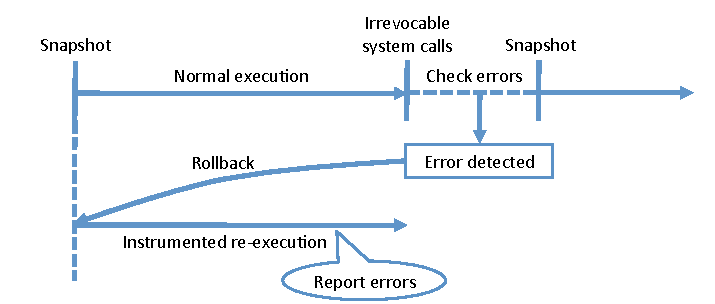
\includegraphics[width=3.3in]{doubletake/figure/overview}
\end{center}
\caption{
Overview of \doubletake{}: execution is divided into epochs at the boundary of irrevocable system calls. 
\label{fig:overview}}
\end{figure}

\doubletake{} aims to reduce the performance overhead of dynamic analyses for memory errors sharing the monotonicity: the evidence of an error is persistent and can be detected after-the-fact. As described in Figure~\ref{fig:overview}, the execution of a program is divided into epochs at irrevocable system calls, discussed in Section~\ref{sec:normal_execution}. Inside each epoch, \doubletake{} allows a program to run at full speed, with the support of checkpointing and very minimum recording overhead. \doubletake{} only checks for evidence of an error when an epoch ends. If an error is detected, \doubletake{} rolls back to the most recent checkpoint and re-execute the program to pinpoint the error.  During the re-execution phase, \doubletake{} can use higher-overhead mechanisms to pinpoint the exact cause of the error. 

Based on this framework, we have implemented three detection tools for heap buffer overflows, use-after-free errors, and memory leaks, which are described in detail in Section~\ref{sec:applications}. 

\doubletake{} employs the following core mechanisms:

\paragraph{Efficient Recording.}
At the beginning of every epoch, \doubletake{} saves a snapshot of program registers, and all writable memory. The epoch ends when the program attempts to issue an irrevocable system call, which is described in Section~\ref{} \CC{here}. \doubletake{} also records the order of thread synchronization operations to support re-execution of parallel programs. \doubletake{} records minimal system state at the beginning of each epoch (like file offsets), which allows system calls that modify this state to be undone if re-execution is required. As a result, most programs require very few epochs and program state checks. We describe the details of each application's state checks in Section~\ref{sec:applications}.

\paragraph{Precise Replay.}
During re-execution, \doubletake{} ensures that all observable system state, system call results, and memory allocations will be the same from the original run. System calls that cannot be replayed, called irrevocable system calls, must be issued at the end of an epoch after detection tools have verified that no errors have occurred. Actually, those system calls consists of the boundary of epochs, which are discussed in Section~\ref{sec:normal_execution}. In practice, most system calls can easily be replayed by handling appropriately. This ensure that most programs run very few integrity checks, and overhead remains low when errors are not detected.

\paragraph{Custom Heap Allocator.}

\doubletake{} replaces the default heap allocator with a BiBOP-style memory allocator, built on HeapLayers~\cite{heaplayers}. \DoubleTake{} pre-allocates a fixed size of memory from its underlying operating system using \texttt{mmap} system calls and satisfies memory allocations from this block by interposing all memory allocation and deallocations. Using the custom memory allocators avoids a big number of sbrk() or mmap() system calls caused by the default memory allocator. In the heap, all heap objects have the block size of {\it power of $2$}, using an object header to mark its status and size information. There is no split and merge operation on heap objects. If the size of an allocation is less than {\it power of 2}, \DoubleTake{} allocates an object with the size of next {\it power of 2}. 






\section{Applications}
\label{sec:applications}

\subsection{Shared Mechanisms}
Before the description of different applications, we listed some shared mechanisms that are used by one or multiple applications. 

\subsubsection{Canary}
\label{sec:canary}
Canary was first proposed by StackGuard~\cite{StackGuard} to find stack smashing problems by placing a canary word before the return address on stack. Those attempts to overwrite the return address should corrupt the canary word at first. Canaries are borrowed to detect buffer overflow ~\cite{overflow:purify}. They are initialized to a special value in the beginning so that modifications of those values indicates the problems. Detection tools can place canary values anywhere in heap memory. \doubletake{} introduces a bitmap to track the locations of canary values, and can check for canaries that have been overwritten. Buffer overflow detection places canary values between heap objects to detect out-of-bounds writes, and use-after-free detection fills freed objects with canaries to detect writes through dangling pointers.

\subsubsection{Watchpoints}
\label{sec:watchpoints}
Watch point mechanism relies on hardware debug registers to monitor memory accesses on specific addresses. Previous work has used this mechanism for their specific targets ~\cite{fastboundschecking, Kivati}. The main target of debug registers is to support software debuggers, e.g. gdb. A small number of watchpoints are available on modern architectures (four on x86). Each watchpoint can be configured to pause program execution when a specific byte or word of memory is accessed. \doubletake{} allows detection tools to set hardware watchpoints before re-execution. Heap Overflow detection tool can use watchpoints to find the instruction(s) responsible for overwriting a canary value.

\subsection{Applications}
\label{sec:applications}

\doubletake{} implements three important applications based on its lightweight dynamic analysis framework. Those applications are implemented in a best-effort way to show the efficiency of our framework. They are not targeted for a complete and novel solution, thus most of mechanisms are borrowed from previous work. 

\begin{figure}[!t]
\begin{center}
\includegraphics[width=3.3in]{doubletake/figure/buffer-overflow-diagram}
\end{center}
\caption{Heap organization used to provide evidence of buffer overflow errors. Object headers and unrequested space within allocated objects are filled with canaries; a corrupted canary indicates an overflow occurred.
\label{fig:buffer-overflow}}
\end{figure}

\begin{figure}[!t]
\begin{center}
\includegraphics[width=3.3in]{doubletake/figure/dangling-pointer-diagram}
\end{center}
\caption{Evidence-based detection of dangling pointer (use-after-free) errors. Freed objects are deferred in a quarantine in FIFO order and filled with canaries. A corrupted canary indicates that a write was performed after an object was freed.
\label{fig:dangling-pointer}}
\end{figure}


\subsubsection{Detection of Heap Buffer Overflows}
\label{sec:overflow}
Buffer overflows occurs when a program writes outside of the range of an allocated object. Buffer overflows can greatly affect the reliability and security of a program. 

\paragraph{Detection.}
To detect heap buffer overflows, \DoubleTake{} puts canaries before and after actual heap objects, which is described in Figure~\ref{fig:buffer-overflow}. This method is borrowed from previous work~\cite{overflow:lbc, AddressSanitizer}.
All heap objects of \doubletake{} are managed by power of two size, adding two words for canaries (16 bytes) for each heap object. For an allocation size not power of two size (a non-aligned object), \doubletake{} rounds it up to the next power of two size class, putting byte-based canaries and word-based canaries immediately after this object. This approach lets \doubletake{} catch overflows as small as one byte. 

Detection happens in the following scenario. At memory deallocation, \doubletake{} checks buffer overflows only for non-aligned objects, with size different with the power of two class. At the end of each epoch, \doubletake{} verifies integrities of all canaries by traversing the bitmap, which marks the placement of canaries and discussed in Section~\ref{sec:canaries}.  Corrupted canaries indicates heap buffer overflows. 

\paragraph{Re-execution.}
\label{sec:overflowreport}
When a program is found to have heap overflows, \doubletake{} rolls back the execution to the most recent checkpoint and re-executes this program.
To precisely identifying instructions responsible for a buffer overflow, \doubletake{} installs a watch point at the address of a corrupted canary before re-execution. When the program is re-executed, any instruction that writes to this address will trigger a debug trap (resulting in a SIGTRAP signal). \doubletake{} then reports the exact call site of trapped instructions, acquired by calling \texttt{backtrace} function. To further help programmer, \doubletake{} can also report the allocation site of an overflowed heap object. 
  
\subsubsection{Detection of Memory Leak}
\label{sec:leak}
Heap memory is leaked when it becomes inaccessible without being freed. Memory leak can greatly reduce the performance and availability of programs, which makes it one of common classes of reported bugs.

\paragraph{Detection.}
\doubletake{} detects memory leak using the same marking mechanism as conservative garbage collection ~\cite{Wilson:1992:UGC:645648.664824}. \doubletake{} marks the reachability of all heap objects: whether a heap object is reachable from the globals, the stack, and registers. Any unreachable object that has not been freed must be leaked. 

In order to compute the reachability from globals, stack, and registers, \doubletake{} starts to put all possible pointers, any eight-byte aligned value falling into the range of the heap, into a work queue. Then \doubletake{} checks all values in the queue using a breadth-first search algorithm: for each value, \doubletake{} verifies whether this value is a valid address inside a heap object; If this valid object is still non-reachable (not checked before), \doubletake{} marks it as reachable and also put all possible pointers inside this object into the work queue. After this step, this value is removed from the work queue. \doubletake{} stops when there is no value in the work queue any more. In this time, all heap objects which is reachable should have been marked. 

After the marking phase, \doubletake{} traverses the whole heap to find leaked objects, those un-reachable non-freed objects. To simplify the marking and checking phase, the status of an object, whether it is freed or reachable are marked in the object header. During this traverse, \doubletake{} recovers the status of every object to un-reachable. \doubletake{} also adds all leaked objects into a global hash table, where each leaked object also keeps information of its starting address and size. 

\paragraph{Re-execution.}
\label{sec:leakreport}
\doubletake{} uses re-execution to find allocation sites for all leaked heap objects. Re-execution proceeds as normal, with an added check in each \texttt{malloc()} function call. When a memory allocation matches the actual size and address of any leaked heap object, 
\doubletake{} reports its call stack, obtaining by using \texttt{backtrace} 
functions of \texttt{glibc} library. 

\subsubsection{Detection of Use-after-free Errors}
\label{sec:danglingpointer}
Memory use-after-free errors occur when an application continues to use a pointer after its corresponding object has been deallocated.
Writing to a freed memory can overwrite the contents of lived objects, leading to unexpected behavior.  

\paragraph{Detection.}
To detect memory use-after-free errors, 
\doubletake{} firstly delays memory re-usage of all freed objects 
by putting them into a quarantine list, same as AddressSanitizer does ~\cite{AddressSanitizer}. 
Those objects in the quarantine list are actually returned back
to the program heap when the total size of freed objects in the quarantine list are larger then a pre-defined threshold or the quarantine list is full.

In order to find evidence of memory use-after-free problems, 
\doubletake{} fills the first 128 bytes of an object, which can be adjustable, with canaries. 

Those canaries are checked before an object is returned back to the program heap or in the end of an epoch. Same as detection of buffer overflows, 
a corrupted canary indicates a use-after-free memory error and must be reported to user. 

\paragraph{Re-execution}
When a program has use-after-free memory errors, \doubletake{} re-executes this program to find out the allocation and deallocation site of corresponding objects and those instructions actually writing them.
%It is possible that multiple instructions can access an object after deallocation.  

To obtain an object's call site of allocation and deallocation, 
\doubletake{} checks starting address of each object during every memory allocation and deallocation. If an object has the same address as those use-after-free objects, its corresponding allocation/deallocation site are saved. To find out those instructions writting a freed object, 
\doubletake{} installs hardware watch points on those violating addresses, which shares the same mechanism as overflow detection.
\doubletake{} reports an use-after-free error, with its allocation site and deallocation site, in order to help programmers locate a memory use-after-free error. 

\section{Implementation} 
\label{sec:implementation}

This section describes the implementation of \doubletake{}, organized by the phases
shown in Figure~\ref{fig:phases}. 
% we should say why we have normal execution and re-execution.
Section~\ref{sec:normal_execution} firstly describes the procedure inside normal execution, which
is the common path for all programs.
Then it describes how to rollback and re-execute a program in Section~\ref{sec:re-execution}, when
there are memory errors detected.

\begin{figure*}[t] {
	\centering
	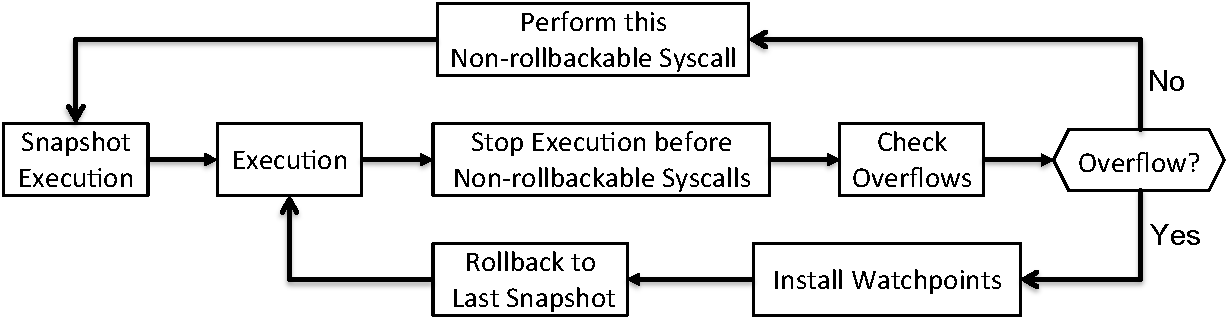
\includegraphics[width=6.5in]{figure/stopgapoverview}
	\caption{\DoubleTake{} diagram. \label{fig:phases}}
	}
\end{figure*}

\subsection{Normal Execution}
\label{sec:normal_execution}

% TODO: Fill in irrevocable system call
\doubletake{} breaks the execution of a program into multiple epochs at irrevocable system calls.
In the beginning of an epoch, \doubletake{} takes a snapshot of the program state. 
During an epoch, \doubletake{} records the program's operations to facilitate re-execution. 
An epoch ends when the program attempts to issue an irrevocable system call, such as \texttt{fork}. 
Before the system call is issued, \doubletake{} checks the program state for errors. 
When no error is detected, \doubletake{} will issue the irrevocable system call and start a new epoch.
If an error is detected, \doubletake{} switches to re-execution mode 
(described in Section~\ref{sec:re-execution}) to gather additional information about memory errors. 

\subsubsection{Starting an Epoch}
{\em Snapshot}. 
At the beginning of every epoch, \doubletake{} take a snapshot of the current program state 
so that we can rollback to this state if there are some errors detected at the end of the current epoch.
A snapshot includes the state of registers (obtained using \texttt{getcontext()}),
and all writable memory, including the globals, the stack and the program heap. 
Read-only memory, such as text segments of a program and libraries, does not need to 
be saved in the snapshot. \doubletake{} analyzes the Linux file \texttt{/proc/self/map} 
to identify the ranges of different memory mappings, including the globals and the stack.
It knows the range of the program heap because of using a customized memory allocator, which is discussed in
Section~\ref{sec:allocator}.  

To snapshot, it first saves the globals of this program and different libraries, 
and then the heap and the stack. 
In the end, it calls \texttt{getcontext} of \texttt{glibc} library to save its execution context.

{\em File Positions}. \doubletake{} records file positions of all opening files
in order to reduce the number of epochs in a program, 
which has been discussed in Section~\ref{sec:syscall}.
For a normal file, \doubletake{} calls \texttt{lseek} to acquire its file position.
For a file opened by \texttt{fopen}-like library calls,
\doubletake{} also saves its corresponding stream additionally.

\subsubsection{Executing an Epoch}
\label{sec:inepoch}
Inside an epoch, \doubletake{} intercepts those library functions involved in system calls 
and handles correspondingly according to the discussion of Section~\ref{sec:syscall}.

For checkpointable system calls, e.g., \texttt{read} and \texttt{write}, since they can 
also be called in socket communications, \doubletake{} has to check whether they 
are working on normal files. In order to speed up the checking process, \doubletake{] is using a hash map to hold file descriptors of all opening files. 
For normal files, reads and writes can be issued normally. 
For reads and writes in network communications, \doubletake{}  ends the current epochs since they are considered to be irrevocable system calls.

For recordable system calls, e.g., \texttt{gettimeofday}, \texttt{time}, and \texttt{mmap},
\doubletake{} records the results of system calls in a First-In-First-Out list, which are necessary to be replayed in re-execution phase if memory errors are detected at the end of the current epoch. 
For \texttt{open}-like library calls, \doubletake{} not only records file descriptors returned by system calls,
but also adds them to the hash map discussed above.  

For delayable system calls, e.g., \texttt{munmap} and \texttt{close}, they are added into a global 
list and are issued in the end of the current epoch after checkings of memory errors.

\subsubsection{Ending an Epoch}
At the end of each epoch, \doubletake{} checks the program state for errors. 
We have implemented error detection for heap buffer overflows (Section~\ref{sec:overflow}), 
memory leakage (Section~\ref{sec:leak}),
and memory use-after-free errors (Section~\ref{sec:danglingpointer}).

When \doubletake{} do not find any memory error, it issues all delayable system calls 
and cleans corresponding lists.
\doubletake{} also cleans recordable system calls
since there is no need to replay those system calls any more.
 
If \doubletake{} finds any memory error, it switches to the re-execution mode, discussed in Section\ref{sec:re-execution}.

\subsection{Rollback and Re-Execution}
\label{sec:re-execution}
When \doubletake{} detects an error, it uses rollback and re-execution to collect additional information to aid programmers in correcting the error. This additional information is either impossible or expensive to collect during normal execution.
In normal execution, it is impossible to know those instructions responsible for buffer overflows and 
memory usage-after-free errors if we do not check every memory access. 
Checking every memory access obviously introduces significant performance overhead, which \doubletake{} avoids. 
It is expensive to acquire call stacks for every memory allocation for detecting memory leakage, \doubletake{} leaves this operation to re-execution phase when memory leakage is detected.
By doing this, \doubletake{} enables programs to run with very low overhead until an error is detected.

\subsubsection*{Preparation}
\doubletake{} does some preparation before it rolls back and re-execute a program with memory errors. 
In order to locate instructions responsible for buffer overflows and memory usage-after-free errors,
\doubletake{} installs watch points on addresses with corrupted canaries, as described in Section~\ref{sec:applications}.
Hardware watch points are configured with debug registers, 
but these registers are only accessible to the kernel. 
Using \texttt{ptrace} function, \doubletake{} forks a child process to install watch points for current process.  

To find the allocation sites and de-allocation sites for memory usage-after-free errors and memory leakage problems, 
\doubletake{} puts all suspected heap objects into a hash map, which are checked for every memory allocation and deallocation. 

Additionally, \doubletake{} calls \texttt{lseek} to recover file positions of all opening files.

\subsubsection*{Rollback}
Regardless of the error detection being used, \doubletake{} must roll back program state 
before the epoch with errors can be re-executed. Before the program stack can be restored, \doubletake{} must switch to a temporary stack since the stack restore process may overwrite its own stack. Next, \doubletake{} restores the state of all writable memory from the epoch's snapshot. Finally, \doubletake{} restores register state with the \texttt{setcontext()} function and re-execution proceeds automatically.

\subsubsection*{Re-Execution}
The main task of re-execution is to collect additional information about different memory errors, which
have been discussed in Section~\ref{sec:applications}. 
In re-execution phase, \doubletake{} repeats the results of recordable system calls by reusing results recorded in normal execution.
For delayable system calls, \doubletake{} turns them to no-op in the re-execution phase.  


\section{Multithreading Support}
\label{sec:multithreading}

This section describes the mulithreading support of \doubletake{}.
A thread is a basic execution unit from the point of view of underlying operating system. 
The order of an execution, greatly affecting memory usage, 
is highly depending on timing, synchronization order and internal scheduling algorithm.   
Thus, it is much more difficult to achieve the target of repeatable memory 
usage for multithreading programs, which is crucial to 
precisely detect buffer overflows or other memory errors.
This section first discusses how to handle epochs in multithreading programs.
After this, it describes the design of heap allocator, suitable for repeatable memory usage.
It then discusses how to handle thread creation and exits specially. 
In the end, it describes how to guarantee deterministic synchronization in the re-execution phase,
which is also crucial for repeatable memory usage.


\subsection{Overview}
\label{sec:mtoverview}

As described in Section~\ref{sec:overview}, \doubletake{} uses irrevocable system calls as 
boundaries for epochs for multithreading programs. 
To simplify description in the following sections, a thread encountering an irrevocalbe system call is 
called as the ``Triggering-Thread''. 

When encountering an irrevocable system call, this Triggering-Thread 
has to stop all existing threads so that all other threads are in a quiecent state, which
has been described in Section~\ref{sec:stopepoch}.
Then it performs memory checkings on the heap as described in Section~\ref{sec:epochend}. 
If there is no buffer overflow, it can perform this irrevocable system call and 
start a new epoch after this system call. 
Before waking up other threads, the Triggering-Thread takes a snapshot for the shared memory at first,
including the heap and globals. 
After a thread is waken up, it only needs to take a snapshot on its own state, 
including its stack and its hardware registers. 

If there are buffer overflows, the Triggering-Thread sets up the shared memory 
for all threads at first.
It recovers the heap and globals by copying from the saved snapshot. 
Then it can wake up other threads. 
However, if the Triggering-Thread is spawed newly in current epoch, 
it has to wait for its parent to start its execution. 

\subsubsection{Epoch}
\label{sec:stopepoch}

It is the duty of a Triggering-Thread to close an epoch.
Whenever this thread meets an irrevocable system call, it has to stop other threads.
\doubletake{} utilizes the ``signal'' mechanism to stop other threads asynchronously.
It signals other threads using SIGUSR2 signal when a thread is in a safe state. 
A thread is considered to be in a unsafe state before this thread finishs a snapshot for itself,
discussed in Section~\ref{sec:threadcreation}.
After sending out all signals, this thread is waiting on a internal conditional variable.
The Triggering-Thread only starts checking buffer overflows after all threads are in quiescence.

However, this SIGUSR2 signal can also be used by user programs. 
In order to differentiate this, \doubletake{} specifically marks on 
a shared flag before signalling so that signal handler can check this in the beginning. 
If this flag is marked, this signal is issued by \doubletake{}. Otherwise, it is issued by
a user program and we can call user registered program instead. 

When other threads receive the signal from the Triggering-Thread, 
they are waiting on an internal conditional variable for instructions from the Triggering-Thread:
it can move forward to next epoch or rollback.
It is worthy noting that inside signal handler we have to utilize a different lock that has not been
used by other places. Otherwise, it is easy to cause deadlock. 

\subsubsection{Customized Heap Allocator}
\label{sec:mtheap}
In order to achive the target of repeatable memory usage, the heap allocator must be designed 
carefully. \doubletake{} first borrows a ``per-thread-heap'' idea from Hoard~\cite{Hoard}. 
\doubletake{} keeps a 1-to-1 mapping between threads and sub-heaps of customized memory allocator. 
The total number of threads and sub-heaps are pre-defined. 
A thread can only allocate memory from its own sub-heap, 
where those sub-heaps can get the memory from a pre-allocated heap 
by allocating a huge block of memory each time. 
After a sub-heap gets a block of memory, its corresponding thread always owns all objects
of this block, called as ``owner'' of this block.
This surely can cause memory blowup problem resolved by Hoard. However, it is 
not the focus of \doubletake{}.   

The ``per-thread-heap'' idea is not enough to guarantee the repeatable memory usage. 
\doubletake{} imposes several additional rules besides this.
Firstly, when \doubletake{} acquires a block of memory from the global pre-allocated heap, it must 
acquire a lock at first, which is guaranteed to be deterministic according to mechanisms 
discussed in Section~\ref{sec:sync}.
This guarantee that every new blocks of each sub-heap is repeatable for re-execution. 
Secondly, when there is a memory deallocation, this freed object can only be returned back  
to its original owner in a safe state. 
If this memory deallocation is issued by the same thread as the owner, then this freed object
can be putted into the owner's free list and be utilized immediately. 
If this memory deallocation is issued by a different thread with the owner, 
which indicates a cross-thread communication,  
then this memory
deallocation are cached into a global list, which only issued in the end of this epoch after 
all threads has been stopped. 
By doing this, we can guarantee all memory usage inside an epoch is repeatable in re-execution phase.
 
\subsection{Thread Creation and Exit}
\label{sec:threadcreation}
Tracking creations and exits of threads is very important because of the following reasons.
First, \doubletake{} has to take snapshots for different threads in the beginning. 
Second, terminination of a thread invokes \texttt{munmap} system calls directly by \pthreads{}, which
can not be intercepted.  
Third, thread creation is considered as a synchronization and has to be recorded. 
Thus, \doubletake{} intercepts \texttt{pthread\_create} calls and changes its start routine 
to a customized function. 
In this customized function, \doubletake{} can record thread creation, take a snapshot and delay thread exit to the end of current epoch. 

\subsubsection{Normal Execution}

\doubletake{} makes \texttt{pthread\_create} to call its customized function as the start routine. 
In this start routine, \doubletake{} first puts this new thread into a global map, which maintains
status of all threads. 
Then it takes a snapshot for this new thread, including stack and hardware registers. 
After this, \doubletake{} can invoke the original routine to actually perform user-defined 
thread function. 

After this user-defined thread function finishes, the control flow returns back to \doubletake{}. 
Basically, \doubletake{} should check whether this thread's parent is joining on this thread or not. 
If this thread's parent is already waiting for its termination, it simply marks the status of 
this thread to be joined and wakes up the joining thread. 
If not, this thread can wait on a thread-private conditional variables. 
\doubletake{} delays a thread exit to the end of current epoch.

\subsubsection{Re-execution}
A thread is waiting for its turn to run if a thread is created in current epoch.    

\subsection{Thread Synchronizations}

\label{sec:sync}

Different order of thread synchronizations can lead to totally different memory uage. 
In order to guarantee deterministic replay of thread synchronizations, previous work
actually forces threads to do synchronizations in a global order and
recordes both lock and unlock operations ~\cite{TERN, PRES}. 
However, forcing a global order of synchronizations can greatly 
reduce parallelism and introduce significant performance overhead.
Also, it is unnecessary to record unlock order too.

Unlike previous approaches, \doubletake{} only records local orders of synchronizations.
Synchronizations on two different synchronization variables can be performaed
in parallel. From a thread's point of view, if a program do not have a race and
all synchronizations of a thread are repeated deterministically, then
\doubletake{} can guarantee memory usage of this thread, which also guarantees to 
repeat the same buffer overflows in re-execution phase. 
If a program do have a race, forcing a global order of synchronizations in the production 
run also can not completely avoid races. This also implies that a global order 
can not always guarantee determinstic memory uage.   
\doubletake{} prefers performance for racey programs, while relying on multiple re-executions 
to repeat buffer overflows if a program does have a race problem. 

\doubletake{} records the order of \texttt{pthread\_mutex\_lock}, conditional wakenup and
different signalling functions.
Signalling functions actually calls system calls, which are handled by the procedure discussed 
in Section~\ref{sec:inepoch}.
 Conditional wakenup is actually related to \texttt{pthread\_cond\_wait},
which actually includes conditional wait and conditional wakenup phases. 
Conditional wait atomically releases mutex and waits on corresponding conditional variable, while conditional wakenup actually locks corresponding mutex before returning. 
Thus, we can turn \texttt{pthread\_cond\_wait} to two operations, \texttt{pthread\_mutex\_unlock} and
\texttt{pthread\_mutex\_lock} correspondingly. So we only record the order of conditional wakenup in
production runs. 
 
\doubletake{} also provides an option to record the order of passing a specified barrier, which it is 
not necessary to do this by default.
It is noted that \doubletake{} do not record the order of unlock operations
and conditional signal operations.
It is totally unnecessary to record unlock operations since recording the order of actual 
lock aquiring operations is enough to guarantee a deterministic replay of critical sections.  
Conditional signal and broadcast operations are skiped for the same reason. 

%why two different synchronization is not important?
How to replay this?
How to handle nested locks? 
The replaying is considerred to be two steps: we first advance thread's entry when we met a .

Maybe pseudo code for this.
 
\subsubsection{Normal Execution}
In production runs, \doubletake{} intercepts all synchronizations and 
records orders of synchronizations, such as lock, conditional waken up and signals, 
based on different synchronization variables. 
It maintains a list for each synchronization variable and records synchronization
events on its corresponding list. 
In order to quickly locate its list when a synchronization is intercepted, \doubletake{}
utilizes original synchronization variables to store addresses of list and actual synchronization
variable. 

For a synchronization event like lock, \doubletake{} records the following information:
which thread issues this synchronization event; what is the result of this synchronization.
A naive implementation is to allocate memory from internal memory allocator every time. 
However, for some applications having significant amount of synchronizations,
memory allocations to record synchronization events contributes much performance overhead. 
For example, \texttt{fluidanimate} runs several times slower because of huge amounts
of synchronizations inside. \doubletake{} uses a pre-allocated list for those recordings. 
More specifically, each thread has a pre-allocated list in the beginning of an epoch. 
When a synchronization occurs on this thread, it can get an entry from this thread and 
record a synchronization event on this entry.
Since \doubletake{} always gets an entry from current thread issuing a synchronization,
there is no need to utilize a lock, which also helps reducing overhead. 
By doing this, \doubletake{} greatly reduce performance overhead of logging synchronization
events. For example, performance overhead of \texttt{fludidanimate} are reduced to around 40\%.

 
\subsubsection{Re-execution}
As described above, for a synchronization event in a thread,
\doubletake{} allocates an entry from current thread to record this synchronization event 
and inserted it into synchronization variable's corresponding list. 
This implies that a synchronization event belongs to two lists, 
a list for all synchronizations of this synchronization variable (SyncVariableList) and 
a list for all synchronizations in a thread (ThreadSyncList). 

Reproducing synchronizations involves in manipulating these two lists using 
{\it sempaphore replay}, similar to TERN ~\cite{TERN}.
We listed the pseudocode of ``lock'' of reproduction runs in Figure~\ref{fig:lockunlock}.
\doubletake{} assigns a semaphore for each thread and controls the order 
of synchronizations based on semaphores: in lock acquisitions, 
a thread waits on its semaphore and advances ThreadSyncList after this semaphore; 
In lock releases, a thread increments the semaphore of next thread on the same 
synchronization variable.
However, \doubletake{} only records local synchronization order, instead of global order,
synchronizations replaying of \doubletake{} is much more subtle.
In order to handle those unsuccessful lock acquisitions, \doubletake{} only waits for a semaphore 
if this lock is successfully acquired in the production run. 
Also, to support nesting locks, in lock acquisitions after {\it advanceThreadSyncList()}, 
\doubletake{} signals current thread if next event of this thread is already 
in its pending list, which means that this thread should have its turn.
For lock releases, \doubletake{} adds next event of SyncVariableList to corresponding thread's 
pending list if the event is not the first event of corresponding thread instead of incrementing
its semaphore directly. 
Since performance of reproduction runs is not the main focus, only occurring for those programs 
having buffer overflows, \doubletake{} are using the same lock for all lists' manipulations to
avoid races.  




\section{Evaluation}
\label{sec:evaluation}

We evaluate \doubletake{} on a quiescent Intel Core 2 dual-processor system with 16GB of RAM running Linux 2.6.18-194.17.1.el5, and version 2.5 of \texttt{glibc}. Each processor is a 4-core 64-bit Intel Xeon, operating at 2.33GHz with a 4MB shared L2 cache a 32KB per-core L1 cache. All benchmarks are built as 64-bit executables using LLVM 3.2 with the clang front-end and \texttt{-O2} optimizations.

Our evaluation measure the runtime and memory overhead of \doubletake{}, and the effectiveness of the heap buffer overflow, memory leak, and use-after-free detectors.

\subsection{Performance Overhead}
\label{sec:perf}

\begin{figure*}[!ht]
	\begin{center}
		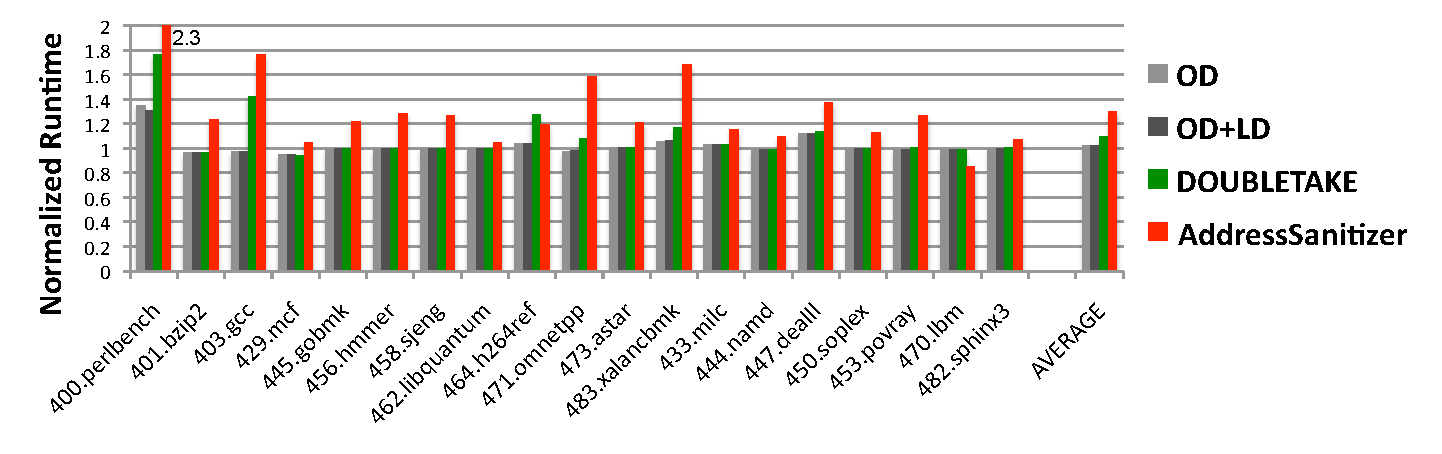
\includegraphics[width=6.5in]{doubletake/figure/perf}
	\end{center}
	\caption{This figure shows the runtime overhead of \doubletake{} (OD - Buffer Overflow Detection, LD - Leak Detection, \doubletake{} - with three detections enabled) and AddressSanitizer, normalized to each benchmark's original execution time. 
%Overhead for Valgrind is reported in Table~\ref{table:valgrind} because the results do not fit on this graph.
\label{fig:perf}}
\end{figure*}

\begin{table}[t]
	\centering
	\begin{tabular}{r|c p{0.1em} r|c}
		\textbf{Benchmark} & \textbf{Overhead} & & \textbf{Benchmark} & \textbf{Overhead} \\
		\cline{1-2} \cline{4-5}
		400.perlbench	& 20.5X	& & 458.sjeng	& 20.3X	\\
		401.bzip2		& 16.8X	& & 471.omnetpp	& 13.9X	\\
		403.gcc			& 18.7X	& & 473.astar	& 11.9X	\\
		429.mcf			& 4.5X 	& & 433.milc		& 11.0X	\\
		445.gobmk		& 28.9X	& & 444.namd		& 24.9X	\\
		456.hmmer		& 13.8X	& & 450.dealII	& 42.8X	\\
	\end{tabular}
	\caption{Valgrind's runtime overhead. \label{table:valgrind}}
\end{table}


We evaluate performance on all C and C++ SPEC CPU2006 benchmarks, 19 applications in total. We compare \doubletake{} with AddressSanitizer and Valgrind. AddressSanitizer is the previous state-of-the-art for detecting buffer overflows and use-after-free errors~\cite{AddressSanitizer}, but cannot detect memory leaks. Valgrind's Memcheck tool is widely used tool to detect buffer overflows, memory leaks, and use-after-free errors~\cite{overflow:valgrind}. 

During performance evaluation, we disable \doubletake{}'s rollback functionality to only measure the overhead of normal execution. \doubletake{} only detects memory errors of the heap, thus AddressSanitizer is run without checks on accesses to the stack and globals, and without checks on read accesses. For each benchmark, we report the average of three runs with the largest input size, except for Valgrind. We only run Valgrind once because of its slowness. 

Performance results of \doubletake{} and AddressSanitizer are shown in Figure~\ref{fig:perf}. Results for Valgrind do not fit on the graph, and are presented separately in Table~\ref{table:valgrind}. On average, \doubletake{} adds only $9\%$ overhead \emph{with all three error detectors enabled}. If \doubletake{} do not detect memory use-after-free errors, the performance overhead is under 3\% on average. AddressSanitizer slows execution by $30\%$ on average, and Valgrind has an average overhead of $19X$ on all evaluated benchmarks. Because Valgrind is running too slow, we haven't finished the evaluation on all benchmarks. Also, we kill a program if it is already running $20\times$ slower, including \texttt{400.perlbench} and \texttt{458.sjeng}. 

% difference across all different tools
For 17 out of 19 benchmarks, \doubletake{} outperforms AddressSanitizer, even with an additional memory leak detection. For 12 benchmarks, \doubletake{}'s runtime overhead is under 3\%. \doubletake{} substantially outperforms Valgrind for all benchmarks. For both \doubletake{} and AddressSanitizer,  \texttt{400.perlbench}, \texttt{403.gcc} and \texttt{447.deallIII} benchmark introduce much more performance overhead than other benchmarks. We also observe that they all introduce much more memory overhead (in terms of absolute value), according our experimental results in Table~\ref{tbl:memoryoverhead}. These significant memory overhead may reduce the ratio of cache efficiency, thus causing performance problem. 



% Difference across all different tools
From the figure, we also notice that detection of memory use-after-free adds about 6\% performance overhead averagely, although most of overhead are coming from \texttt{400.perlbench}, \texttt{403.gcc} and \texttt{464.h264ref} benchmark. As described in Section~\ref{sec:danglingpointer}, \doubletake{} has to fill every freed object up to 128 bytes with canaries and check those canaries when a freed object is released to the program heap. If an application has a big number of memory allocation and de-allocation, these operations consist of most of performance overhead. 




Table 3 shows detailed benchmark characteristics. The “Processes” column shows the number of different invocations in the input set. The number of epochs is significantly lower than the number of system calls because of \doubletake{}'s lightweight system call handling. Benchmarks with the highest overhead run a substantial number of epochs (perlbench and h264ref) and make a large number of malloc calls (gcc, omnetpp, and
xalancbmk).



\subsection{Memory Overhead}
\label{sec:memoverhead}

\begin{table}[t]
\centering
\begin{tabular}{l|c|c|c|}
\textbf{ \small Benchmark} & \textbf{\small Original} &  \textbf{\small AddressSanitizer} & \textbf{\small \doubletake{} } \\
\hline
400.perlbench & 656 &	1481 & 1977 \\
401.bzip2	& 870 &	1020 &	1003 \\
403.gcc	& 683 &	2293 &	1583 \\
429.mcf	& 1716 &	1951 &	1994 \\
445.gobmk &	28 &	137 &	58 \\
456.hmmer &	24 &	256 &	129 \\
458.sjeng & 179 & 220 &	203 \\
462.libquantum	& 66 &	144 &	131 \\
464.h264ref	& 65 &	179 &	247 \\
471.omnetpp	& 172 &	538 &	291 \\
473.astar	& 333 &	923 &	477 \\
483.xalancbmk &	428 & 1149 &	801 \\
433.milc	& 695 &	1008 &	917 \\
444.namd	& 46 &	79 &	92 \\
447.dealII	& 514 &	2496 &	1727 \\
450.soplex	& 441 &	1991 &	1654 \\
453.povray	& 3 &	133 &	50 \\
470.lbm	& 418 &	496 &	470 \\
482.sphinx3 &	45 &	181 & 98 \\
\hline
Total & 7386 & 16678 & 13906 \\
\hline
\end{tabular}
\caption{Memory Usage of \doubletake{} and AddressSanitizer(MB).\label{tbl:memoryoverhead}}
\end{table}


\begin{figure*}
\begin{center}
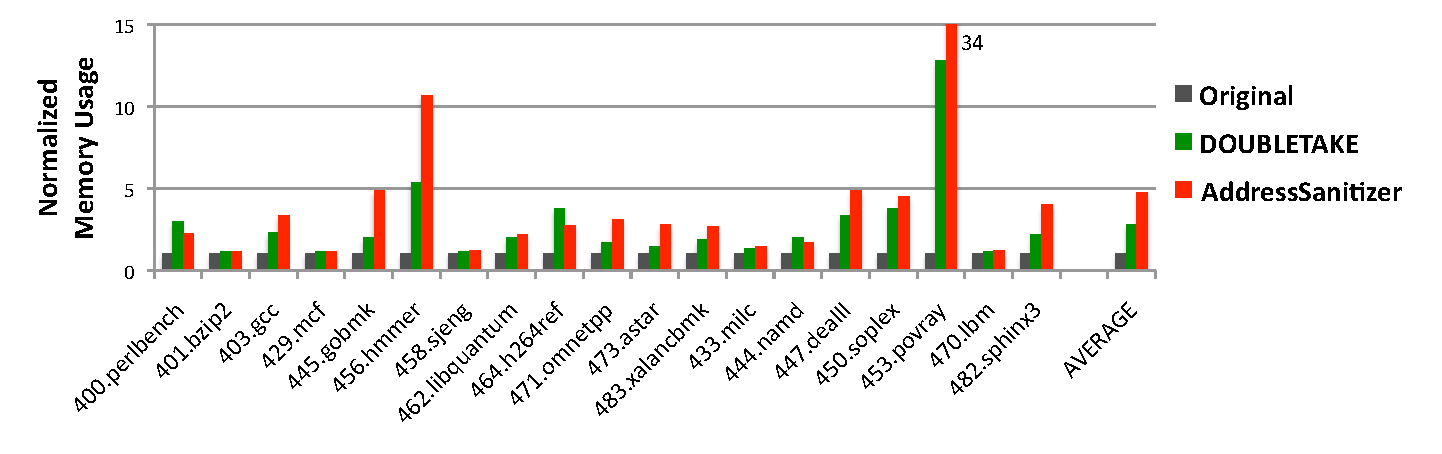
\includegraphics[width=6.5in]{doubletake/figure/memory}
\end{center}
\caption{
Memory overhead of \doubletake{} and AddressSanitizer.
\label{fig:memory}}
\end{figure*}

Memory overhead of \doubletake{} comes from the following aspects. Firstly, snapshot in the beginning of each epoch, by backing up the globals, the heap and the stack, contributes the most significant memory overhead of \doubletake{}. Snapshot can double the memory usage. However, the first snapshot happening in the beginning of a program normally doesn't take too much memory since there is no heap usage at all. Thus, this explains why \texttt{401.bzip2}, \texttt{429.mcf}, \texttt{458.sjeng},  \texttt{433.milc}, and \texttt{470.lbm} have less than $2\times$ memory overhead. Secondly, recording results of system calls introduce some memory overhead. Additionally, different applications may introduce different memory overhead. For the detection of heap buffer overflows and memory leakage, \doubletake{} adds canaries around each heap object and maintains a bit map to indicate canary locations. For the detection of memory usage-after-free errors, \doubletake{} delays memory re-usage by putting freed objects into a quarantine list, which also introduces constant additional memory overhead. 

We only evaluate the physical memory overhead here because \doubletake{} pre-allocates a huge block of heap, which is 4GB virtual memory and should not be counted as memory overhead. Also, we all only care about physical memory overhead when virtual memory overhead is practically infinite in 64bit machine. Proportional set size (PSS) in \texttt{/proc/self/smaps} reflects physical memory increase on the existing system by running an application. Thus, we periodically collect this data and use the sum of different memory mappings as total physical memory usage. We presents the normalized memory overhead of running different benchmarks in Figure~\ref{fig:memory}. We also list the actual memory usage of \doubletake{} and AddressSanitizer in Table~\ref{tbl:memoryoverhead}.

From Figure~\ref{fig:memory}, \doubletake{}'s memory overhead is 2.8$\times$, while AddressSanitizer's overhead is 4.8$\times$. For \texttt{453.povray} and \texttt{464.h264ref}, both AddressSanitizer and \doubletake{} has very high normalized memory overhead because the original memory usage of this benchmark is extremely low, only 3 and 24 megabytes. But for other benchmarks, both AddressSanitizer and \doubletake{} has memory overhead lesss than $5\times$. For all benchmarks except \texttt{400.perlbench} and \texttt{444.namd}, \doubletake{} has lower memory overhead. 
From Table~\ref{tbl:memoryoverhead}, AddressSanitizer totally spends about 20\% more memory than \doubletake{}. In total, \doubletake{} memory overhead is less than 2$\times$ of original memory usage. 

\subsection{Effectiveness}
\label{sec:effect}


We use \doubletake{} to find errors in both the SPEC CPU2006
benchmark suite and a suite of real applications.

\emph{Benchmarks.} During the evaluation of SPEC CPU2006 benchmarks, \doubletake{} detected a one-byte heap buffer overflow
 in \texttt{perlbench}, which can not be detected by AddressSanitizer. \doubletake{} also detected a big number of memory leaks in \texttt{perlbench} and \texttt{gcc}, which has been verified using Valrind.

\emph{Real Applications.} For buffer overflows, we have evaluated the effectiveness on  six real applications. \texttt{libHX} has been evaluated in previous work~\cite{overflow:Cruiser}. \texttt{bzip2}~\cite{bzip2overflow} and \texttt{vim} ~\cite{vimoverflow} are got from Red Hat Bugzilla. Other benchmarks are from bugbench~\cite{bugbench}. We especially turn global array buffer overflow in \texttt{bzip2}, \texttt{gzip}, and \texttt{polymorphy} to heap buffer overflows. \doubletake{} successfully caught all these found heap buffer overflows. The buffer overflows we observed in these applications are triggered by specific inputs, which are difficult to detect during development. \doubletake{}'s overhead is low enough to be enabled in deployment, which would make it possible to detect these bugs in the field.
\doubletake{} also detects memory leaks in \texttt{gcc-4.4.7} and \texttt{vim}.


\chapter{Processes-As-Threads Framework}
\label{sec:sheriffframework}


%%%%%%%%%%%%%%%%%%%%%%%%%%%%%%%%%%%%%%%%%%%%%%%%%%%%%%%
% How to replace threads with processes ?
%  1. Replacing pthread_create() with fork
%  2. How to achieve the same semantics with multithreading? 
%     a. Thread Creation and Exits
%     b. Synchronizations?
%     c. Custom Memory Allocator. how to share memory across different threads
%     d. Twining and diffing mechanism
%
%%%%%%%%%%%%%%%%%%%%%%%%%%%%%%%%%%%%%%%%%%%%%%%%%%%%%%%

\sheriff{} extends the processes-as-threads idea, first introduced in Grace~\cite{grace}, to be a drop-in replacement library of \pthreads{}. It interposes those thread-spawning calls and replaces them with \texttt{clone} system calls with \texttt{CLONE\_FILES} flag. Thus, different processes have separate address spaces and signal handlers, but share all opened files (Section~\ref{sec:threadcreat}). Because of that, different processes can isolate their executions and employ page-based ``per-thread'' memory protection. In order to achieve the same semantics of multithreading programs, \sheriff{} turns synchronizations into process-based synchronizations (Section~\ref{sec:sheriffsync}), runs the regions between synchronizations in the isolation mode (Section~\ref{sec:sherifftransaction}), and commits process-private changes to the shared mapping in order to achieve the  semantics of shared memory, like multithreading programs(Section~\ref{sec:sharedmemory}). 

\begin{figure*}[!h]
\centering
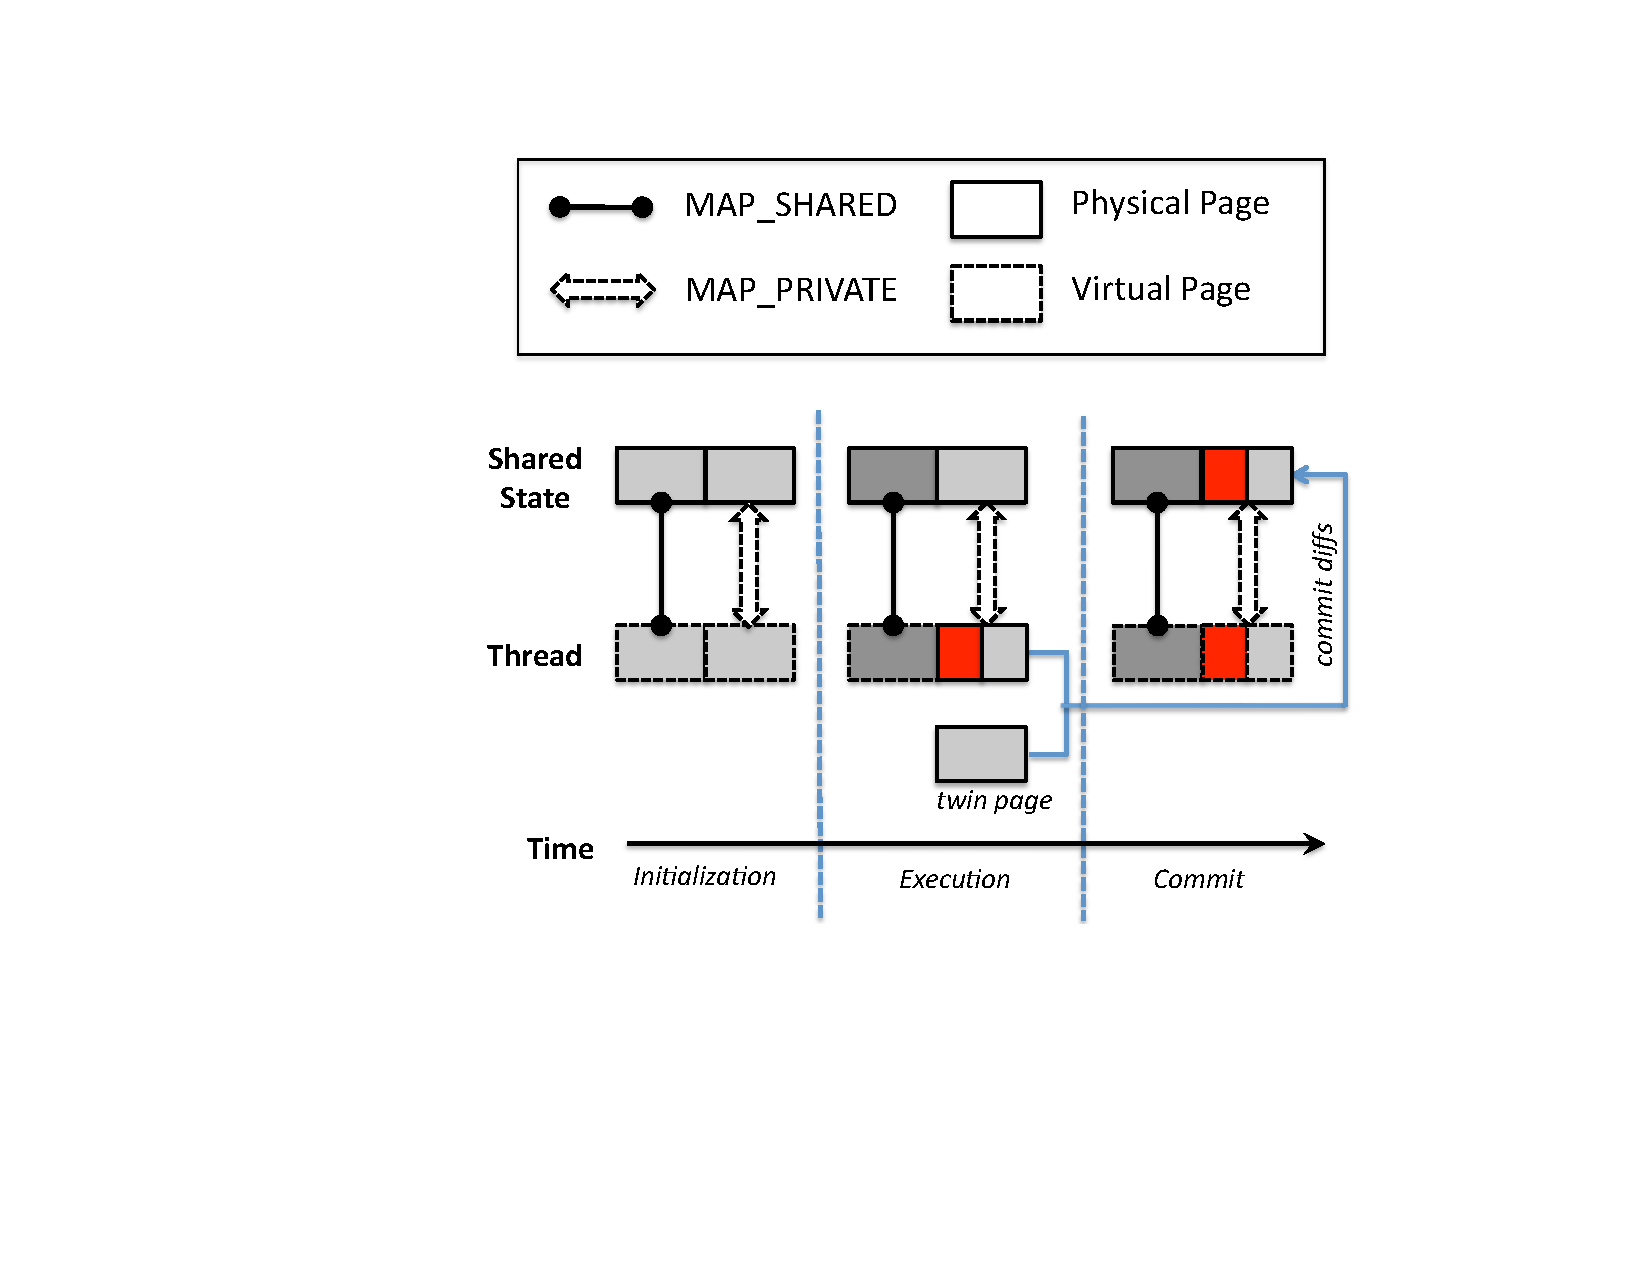
\includegraphics[height=5in]{sheriff/figure/sheriffframework.pdf}
\caption{
\Sheriff{} replaces threads with processes, thus it enables page-based ``per-thread'' memory protection and memory isolation. Upon synchronization points, local changes of different ``threads'' are committed to the shared state by comparing the difference between those working pages and their twin pages. \label{fig:overview}}
\end{figure*}

\section{Thread Creation and Exit}
\label{sec:threadcreat}

For thread creations, \sheriff{} interposes \texttt{pthread\_create()} functions and replaces them with \texttt{clone} system calls. 
By taking advantage of a feature of Linux that allows
selective sharing of memory and file descriptors, \sheriff{}
sets the \texttt{CLONE\_FILES} flag when creating new processes, resulting in child processes with different address spaces but the same shared file descriptor table. However, this attribute may not be applicable to other systems, e.g., Solaris. That would require shims on I/O operations to allow processes to share open file descriptors by sending
them over UNIX domain sockets~\cite[Section 17.4]{unixprogramming}.

For newly spawned threads, \sheriff{} specifically invokes the \texttt{exit} function in order to exit those processes. For \texttt{pthread\_join}, joiners call \texttt{waitpid} to wait for a corresponding process to complete.  

\section{Synchronizations}
\label{sec:sheriffsync}

\sheriff{} supports the full range of synchronizations, including mutexes, conditional variables, barriers, and signals. 

By definition, synchronization is used to coordinate activities and data accesses among different threads. For example, a program calls \texttt{mutex\_lock()} before accessing the shared data. Leveraging on the processes-as-threads mechanism, \sheriff{} actually runs the regions between synchronizations in an isolated mode, which actually divides a program execution into different ``transactions.'' In the same transaction, all reads/writes happen only on private pages after the first write operation on those pages. Reads still perform on the shared mapping directly if a page is not written by the current thread.

At synchronization points, \sheriff{} commits those private changes of each thread to the shared mapping in order to achieve the shared memory semantics of multithreading programs. Detailed implementation about the execution inside a transaction is discussed in Section~\ref{sec:sherifftransaction}. 

It is noted that the transaction concept here is different from that of transactional memory~\cite{transaction}. \sheriff{} does not support rollback and favors more on a longer transaction to better amortize the overhead. 

\sheriff{} turns threads into processes and runs an application in an isolated mode when there is no synchronization. But this isolation mechanism does not work for those synchronization variables. For example, in the mutex\_lock(), if a process only updates its private page holding this lock variable, then this update is not seen by other processes, which can cause multiple processes to enter into the same critical section concurrently. In order to coordinate across different threads, \sheriff{} invokes process-based synchronizations on those synchronization variables that are shared across different processes, shown in Figure~\ref{fig:synccode}. Whenever there is a synchronization, \sheriff{} ends the current transaction, gets its process-shared variable, and synchronizes on this variable by using a process-based synchronization. To quickly locate its process-shared variable for a synchronization variable, \sheriff{} simply stores the pointer of it into the first word of this synchronization variable. 
 
\begin{figure}[!t]
\small
\begin{lstlisting}[style=tt]
void sync(var) {
  endTransaction();
  realVar = getRealVariable(var);
  sync_process_based(realVar);	
  beginTransaction();
}
\end{lstlisting}
\caption{Pseudo-code for a synchronization.\label{fig:synccode}}
\end{figure}

\section{Shared Memory Semantics}
\label{sec:sharedmemory}

In order to create the shared memory illusion for the process-as-threads framework, \sheriff{} employs the memory-mapped files to share the heap and globals across different processes, but not the stack. Different threads are using their own stacks and the stack is not used a cross-thread communication in general.

\sheriff{} creates two different mappings for both the heap and the globals. One is a shared mapping, which is used to hold the shared state. Another is a private, copy-on-write(COW) mapping (per-process) that each process works on directly.

Private mappings are linked to shared mappings through the same memory mapped file. Reads initially go to the shared mapping until the first write on a page. After the first write operation, both reads and writes happen on the private mappings only. In order to achieve the shared memory illusion, \sheriff{} commits the current thread's local changes to the shared mapping at synchronization points using the Twinning-and-diffing mechanism described in Section~\ref{sec:twinning-and-diffing}. More details of this are discussed in Section~\ref{sec:sherifftransaction}.

In the initialization phase, \sheriff{} checks its \texttt{/proc/pid/maps} file to find the range of its globals and creates a shared mapping for the globals. For the heap, \sheriff{} uses a fixed-size memory mapping, which is discussed in Section~\ref{sec:customheap}. 

\subsection{Twinning and Diffing mechanism}
\label{sec:twinning-and-diffing}
In order to find out those local changes made by each thread, \sheriff{] borrows the twin page mechanism, which is introduced in TreadMarks and Munin~\cite{dsm:treadmarks, dsm:munin} for tracking modifications on a page in the distributed share memory system.

The basic idea is to create an additional ``twin'' page before the actual modification, with the help of memory protection. After that, \sheriff{} creates an identical ``working'' page for each thread using the memory copy-on-write mechanism. At synchronization points, \sheriff{} compares a ``twin'' page and its ``working'' page using a byte-by-byte comparison in order to find out those changes made by a thread: the difference of two pages simply implies the local changes made by the current thread. 

\subsection{Custom Memory Allocation}
\label{sec:customheap}

For the program heap, \sheriff{} replaces the default heap allocator with a BiBOP-style memory allocator, built on HeapLayers~\cite{heaplayers}. \sheriff{} pre-allocates a fixed chunk of memory from its underlying operating system using \texttt{mmap} system calls and satisfies memory allocations from this block by interposing all memory allocations and deallocations. In the heap, all heap objects have the block size of {\it power of $2$}, using an object header to mark its status and size information. There is no split and merge operation on heap objects. If the size of an allocation is less than {\it power of 2}, \sheriff{} allocates an object with the size of the next {\it power of 2}.

In order to minimize possible false sharing induced by the memory allocator, \sheriff{} borrows a ``per-thread-heap'' idea from Hoard~\cite{Hoard}. \sheriff{} divides the heap into a fixed number of sub-heaps (currently 16). The metadata for each sub-heap is also shared by different threads and protected by a cross-process mutex.  A thread can only allocate memory from its own sub-heap. When an object is freed, this object is returned to the subheap owned by the current thread. Since the subheap of each thread is allocated from different pages, this custom memory allocator is unlikely to allocate two objects from different threads on the same cache line, helping reduce the false sharing effect. 

\section{Execution of a Transaction}
\label{sec:sherifftransaction}

This section walks through an example of \sheriff{}'s execution from the beginning of a transaction to its termination. 

\emph{Transaction Begin:}
At the beginning of every transaction, \sheriff{} write-protects all shared pages so that later writes to these pages can be caught by handling SEGV protection faults.  

\emph{Inside a Transaction: }
Inside each transaction, \sheriff{} runs at the
same speed as a conventional multithreaded program for program reads. However, the first write to a protected page triggers a page fault that \sheriff{} handles: in the page fault handler,\sheriff{} obtains an exact copy of this page (a ``twin'' page), records the page holding the faulted address, and then unprotects this page so that future accesses run at full speed. Since \sheriff{} only exposes the private mapping to the program, write accesses on a private mapping actually create a ``working'' page for every page written inside a transaction. 

Although protection faults are expensive,
these costs are amortized over the entire transaction because each page only incurs at most one page fault per transaction.
 
\emph{Transaction End:}
At the end of each transaction, at thread exits and before synchronization points, \sheriff{} commits local changes of a thread to the shared mapping to achieve the shared memory semantics. \sheriff{} commits only the differences between those ''twin'' pages and their ``working'' pages.

After those local changes are committed, \sheriff{} reclaims memory holding ``twin'' pages and ``working'' pages. \sheriff{} issues the \texttt{madvise} call, with the \texttt{MADV\_DONTNEED} flag, to discard those ``working'' pages. 


\chapter{\dthreads{}:Efficient Deterministic Multithreading}

\label{sec:introduction}

The advent of multicore architectures has made multithreaded
programming increasingly necessary, but writing multithreaded programs remains painful. It is notoriously far more challenging to write concurrent programs than sequential ones because of the wide range of errors it can cause, including deadlocks and race conditions~\cite{havender,76897,130623}. Because thread interleavings are non-deterministic, different runs of the same multithreaded program can unexpectedly produce different results. These ``Heisenbugs'' greatly complicate debugging, and eliminating them requires extensive testing to account for possible thread interleavings~\cite{DBLP:conf/icse/BallBHMQ09,DBLP:conf/asplos/BurckhardtKMN10}.


Instead of testing, one promising alternative approach is to attack the problem of concurrency bugs by eliminating its source: non-determinism. A fully \emph{deterministic multithreaded system} would prevent Heisenbugs by ensuring that executions of the same program with the same inputs always yield the same results, even in the face of race conditions in the code. Such a system would not only dramatically simplify debugging of concurrent programs~\cite{Carver:1991:RTC:624586.625040} and reduce their attendant testing overhead, but would also enable a number of other applications. For example, a deterministic multithreaded system would greatly simplify record and replay for multithreaded programs~\cite{Choi:1998:DRJ:281035.281041,LeBlanc:1987:DPP:32387.32396}
and the execution of multiple replicas of multithreaded applications for fault tolerance~\cite{deterministic-process-groups,1134000,224058,replicant-hotos}.

Several recent software-only proposals aim at providing
deterministic multithreading, but these all suffer from a variety of disadvantages. Language-based approaches are effective at removing determinism but require programmers to write code in specialized languages, which can be impractical~\cite{Bocchino:2009:TES:1640089.1640097,Burckhardt:2010:CPR:1869459.1869515,Simpson:1999:SEE:330346.330357}. Recent deterministic systems that target legacy programming languages
(especially C/C++) are either incomplete or impractical. Kendo ensures determinism of synchronization operations with low overhead, but does not guarantee determinism in the presence of data races~\cite{1508256}. Grace prevents all concurrency errors but is limited to fork-join programs, and although it is efficient, it can require code modifications to avoid large runtime overhead~\cite{grace}. CoreDet, a compiler and runtime system, enforces deterministic execution for arbitrary multithreaded C/C++ programs~\cite{Bergan:2010:CCR:1736020.1736029}. However, it exhibits prohibitively high overhead (running up to $8\times$ slower than \pthreads{}; see Section~\ref{sec:evaluation}) and generates thread interleavings at arbitrary points in the code, complicating program debugging and testing.

\hspace{1em} \\
\noindent
\textbf{Contributions:}
This paper presents \textbf{\dthreads{}}, an efficient deterministic runtime system for multithreaded C/C++ applications. \dthreads{} guarantees deterministic execution of multithreaded programs even in the presence of data races (notwithstanding external sources of non-determinism
like I/O): given the same sequence of inputs, a program
using \dthreads{} always produces the same output. \dthreads{}'
deterministic commit protocol not only eliminates data races but also prevents lock-based deadlocks.

\dthreads{} is easy to deploy: it works as a direct replacement for the \pthreads{} library, requiring no code modifications or
recompilation. \dthreads{} is also efficient. \dthreads{} leverages process isolation and virtual memory protection to track and isolate concurrent memory updates, which it deterministically commits. Not only does this approach greatly reduce overhead versus approaches that use software read and write barriers, it also eliminates cache-line based false sharing, a notorious performance problem for multithreaded
programs. These two features combine to enable \dthreads{} to nearly match or even exceed the performance of \pthreads{} for the majority of the benchmarks examined here. \dthreads{} thus marks a significant improvement over the state of the art in deployability and performance, and provides promising evidence that fully deterministic multithreaded programming may be practical.

\section{\dthreads{} Overview}
Figure~\ref{fig:nondeterminism} shows an example multithreaded program that, because of data races, non-deterministically produces the outputs ``1,0,'' ``0,1,'' and ``1,1.''  The order of instructions are changed from one execution to the other, resulting in these nondeterministic outputs. Using \dthreads{}, this program will \emph{deterministically} produce the same output-``1,1'' . Although this output can be a undesired one, the fact that results are always reproducible would make it easy for developers to reproduce and locate data races inside parallel programs.

\begin{figure}[h]
{\centering
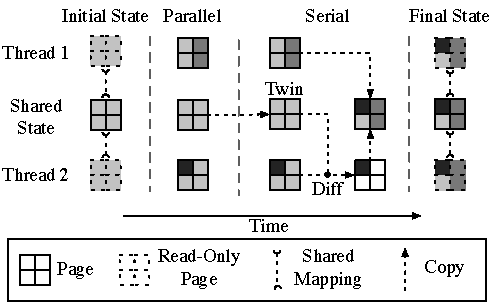
\includegraphics[width=6in]{dthreads/figure/architecture-diagram}
\caption{An overview of \dthreads{} execution.\label{fig:architecture}}
}
\end{figure}

\dthreads{} employs the following mechanisms to ensure the deterministic execution, illustrated by Figure~\ref{fig:architecture}: 

\textbf{Isolated Memory Access:} In \dthreads{}, threads are actually running as separate processes with private and shared views of memory, which is based on the \sheriff{} framework. Because processes have separate address spaces, \dthreads{} can isolate executions of different ``threads''. \dthreads{} uses this isolation mechanism to control the visibility of memory state, so that the updates made by a thread can not be seen by other threads if those updates are not committed explicitly to the shared mapping. By doing this, we guarantee that each ``thread'' can operate independently until synchronization points. Implementation of this is discussed in depth in Section~\ref{sec:threadsasprocs}.

\textbf{Deterministic Memory Commit:} 
Multithreading programs use shared memory for communication, thus \dthreads{} must propagate a thread's changes to be seen by other threads. To guarantee determinism, \dthreads{} should publish updates of different threads in a deterministic order at deterministic points.

\dthreads{} actually commits the changes of a thread to the shared state in sequence at synchronization points. These points includes thread creation and exit; mutex lock and unlock; condition variable wait and signal; posix sigwait and signal; and barrier waits. Commits are ordered using a global ``token'' that is passed from one thread to the next; a thread can only commit when it holds the token.  The token-passing protocol is described in Section~\ref{sec:schedule} and the implementation of synchronization primitives is described in Section~\ref{sec:synchronization}.

\dthreads{} relies on the twinning and diffing mechanism to find out local changes of different threads, which has been discussed in Section~\ref{sec:twinning-and-diffing}. 

\textbf{Deterministic Synchronization:}
There is no deterministic guarantee on synchronizations under existing operating systems. Thus, \dthreads{} re-implements the full range of pthreads synchronization primitives and discusses  them in details in Section~\ref{sec:synchronization}. 

\hspace{1em} \\
\noindent
\textbf{Fixing the data race example} \\
About the example program in Figure~\ref{fig:nondeterminism},  \dthreads{} effectively isolates the execution from each thread until it completes, and then orders updates from different threads by thread creation time using a deterministic last-writer-wins protocol.

In the beginning of every execution, thread 1 and thread 2 have the same view of shared state, with a = 0 and b = 0. Because changes by one thread to the value of a or b will not be made visible to the other until this thread exits, both checks on two threads on line 2 will be true. Thread 1 sets the value of a to 1, and thread 2 sets the value of b to 1. These threads then commit their updates to the shared state and exit, with thread 1 always committing before thread 2. The main thread then should always prints “1, 1” on every execution.

This determinism not only enables record-and-replay and replicated execution, but also effectively converts Heisenbugs into “Bohr” bugs, making them reproducible. In addition, \dthreads{} optionally reports any conflicting updates due to racy writes, further simplifying debugging.


\section{\dthreads{} Architecture}

\begin{comment}
Because multithreaded programs frequently use updates to shared memory to communicate, \dthreads{} must implement a mechanism to expose one thread's updates to all other threads.  At the beginning of a transaction, all shared pages are protected, and can only be read by threads.  When a thread attempts to modify a shared page a local working copy is created, leaving the shared page unmodified.  At commit time, a ``twin'' copy of all modified pages is created.  Every page is compared to its twin (using a byte-wise diff) and modified bytes are copied back to the shared state.  Unlike transactional memory, conflicting changes do not result in rollbacks with \dthreads{}.  Further details are described in Section~\ref{sec:sharedmemory}.
\end{comment}


\label{sec:dthreads-architecture}
This section describes \dthreads{}’ key algorithms—memory isolation, deterministic (diff-based) memory commit, deterministic synchronization, and deterministic memory allocation—as well as other implementation details.

\subsection{Isolated Memory Access}
\label{sec:threadsasprocs}

In order to achieve the deterministic memory access, 
\dthreads{} isolates memory accesses among different
threads between commit points, and commits the updates of each thread deterministically. \dthreads{} is based on the \sheriff{} framework, discussed in Section~\ref{sec:sheriffframework}.

Relying on the \sheriff{} framework, \dthreads{} isolates  memory access among different threads: different threads can only see their own local changes. Additionally, \dthreads{} shims the \texttt{getpid()} function to return a single, globally-shared process identifier. 

\subsubsection{Deterministic Thread Index}
\label{sec:threadindex}

POSIX does not guarantee deterministic process or thread identifiers. To avoid exposing this nondeterminism to threads running as processes, \dthreads{} shims the \texttt{pthread\_self()} function in order to return an internal thread index.  This internal thread index is managed using a single global variable that is incremented on thread creation.  This unique thread index is also used to manage per-thread heaps and as an offset into an array of thread entries.

\subsubsection{Shared Memory}
\label{sec:stackandheap}

In order to create the illusion that different threads are sharing the same address space, \dthreads{} uses memory mapped files to share the globals and heap across different processes.

As discussed in Section~\ref{sec:sharedmemory}, \dthreads{} creates two different mappings for both the heap and the globals.  One is a shared mapping, which is used to hold shared state. The other is a private, copy-on-write (COW) per-process mapping that each process works on directly.  Private mappings are linked to the shared mapping through the single fixed-size memory mapped file. Reads initially go directly to the shared mapping,
but after the first write operation, both reads and writes are entirely private.

Memory allocations are issued from the shared heap memory using a scalable per-thread heap organization loosely based on Hoard~\cite{BergerMcKinleyBlumofeWilson:ASPLOS2000} and built using HeapLayers~\cite{BergerZornMcKinley:2001}.  \dthreads{} divides the heap into a fixed number of sub-heaps (currently 16).  Each thread uses a hash of its thread index to find the appropriate sub-heap.

\subsection{Deterministic Memory Commit}
\label{sec:sharedmem}

\begin{figure}
{\centering 
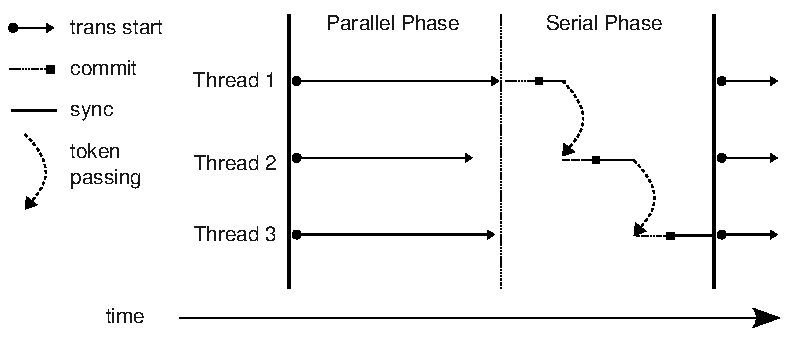
\includegraphics[width=3.25in]{dthreads/figure/phase}
\caption{An overview of \dthreads{} phase. Program execution with \dthreads{} alternates between parallel and serial phases.\label{fig:phase}}
}
\end{figure}

Figure~\ref{fig:phase} illustrates the execution of programs under \dthreads{}.  To guarantee determinism, \dthreads{} isolates memory accesses in parallel phases. In parallel phases, memory accesses work on private copies after the first write operation and updates are not shared across threads.  When a synchronization point is reached, updates are exposed in deterministic order.  This section describes the mechanisms used to guarantee deterministic commit order, and the details of commits to shared memory.

\subsubsection{Fence and Token}
\label{sec:schedule}

\dthreads{} places internal fences between the parallel and serial phases. \dthreads{} re-implements the fence because the standard \pthreads{} barrier mechanism does not support dynamic changes of threads number. 

\begin{figure}
\begin{lstlisting} [style=tt]
void waitFence(void) {
  lock();
	
  while(!isArrivalPhase()) { 
    CondWait();
  }

  waiting_threads++;
  if(waiting_threads < alive_threads) {
    while(!isDeparturePhase()) {
      CondWait();
    }
  } 
  else {
    setDeparturePhase();
    CondBroadcast();
  }

  waiting_threads--;
  if (waiting_threads == 0) {
    setArrivalPhase();
    CondBroadcast();
  }

  unlock();
}

\end{lstlisting}
\caption{Pseudocode for the internal fence.\label{fig:internalFence}}
\end{figure}

Figure~\ref{fig:internalFence} shows the pseudocode code for the internal fence. Threads must wait at the fence until all threads from the previous fence have departed. Then those threads are waiting on the fence until all alive threads  have entered into the same fence(lines 8-11). 
The last thread entering the fence initiates the departure phase and wakes up all threads on the fence(lines 14-15). As threads leave the fence, they decrement the waiting thread count.  The last thread to leave sets the fence to the arrival phase and wakes any waiting threads (lines 19-21).

To reduce overhead, whenever the number of running threads is
less than or equal to the number of cores, waiting threads block by spinning rather than by invoking relatively expensive cross-process \pthreads{} mutexes. When the number of threads exceeds the number of cores, \dthreads{} falls back to using \pthreads{} mutexes.

\begin{figure}
\begin{lstlisting} [style=tt]
void waitToken() {
  waitFence();
  while(isNotMyToken()) { yield(); }
}
void putToken() {
  passTokenToNextOfTokenQueue();
}
\end{lstlisting}
\caption{Pseudocode for waitToken and putToken. 
\label{fig:token}}
\end{figure}

Another key mechanism of \dthreads{} is using the token to order memory commits and synchronizations. The token implementation is listed in Figure~\ref{fig:token}. The token is a shared pointer that points to the next runnable thread entry, which guarantees the global order for all operations in serial phases.  

\dthreads{} introduces two subroutines to manage tokens.  The\texttt{waitToken()} function first waits at the internal fence and then waits to acquire the global token
in order to enter serial mode. The \texttt{putToken()} function passes the token to the next waiting thread. 

As shown in Figure~\ref{fig:phase}, it is very important for a thread to wait at the internal fence before a thread enters into serial phases or before a thread leaves serial phases, even for a thread that is guaranteed to have the token next. Memory commits by a thread can affect other threads' behavior. 

\subsubsection{Commit Protocol}
\begin{figure}
{\centering
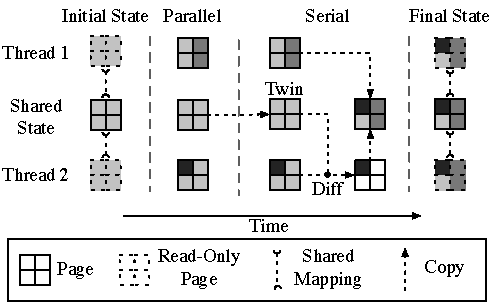
\includegraphics[width=5in]{dthreads/figure/architecture-diagram}
\caption{An overview of \dthreads{} execution.\label{fig:architecture}}
}
\end{figure}

Figure~\ref{fig:architecture} shows the steps to capture modifications to shared state and expose them in a deterministic order.  

At the beginning of the parallel phases, different threads have a read-only mapping for all shared pages. If a thread writes to a shared page during the parallel phases, this write is trapped in order to create a private copy and a twin page for this shared page. After that, reads and writes on this page happen on the private copy only. Reads go directly to the shared memory and are not trapped.  

In the serial phases, threads first commit their local changes happening in parallel phases one at a time, guided by the global token.  The first thread to commit to a page can directly copy its private copy to the shared state, but subsequent commits must copy only the modified bytes. To find out those modifications, \dthreads{} compares those private copies against those twin pages, creating from the shared mapping before actual modification.  After a thread commits its local changes, it issues synchronizations before it passes the token to next thread. 

In the end of serial phase, every threads have to wait at the fence in order to enter into the next parallel phase. 

\subsection{Deterministic Synchronization}
\label{sec:synchronization}
\dthreads{} supports the full range of synchronizations of
\pthreads{} APIs, including locks, conditional variables, barriers and different types of thread exit. Because the \sheriff{} framework can not provide any determinism guarantee, \dthreads{} re-implements all synchronizations as the following.

\subsubsection{Locks}
\dthreads{} uses the global token to guide synchronizations during the serial phases. Before a thread is acquiring a lock while current thread does not have the token, it has to wait for the global token. 

\dthreads{} treats multiple locks as the same one, which  possibly compromise the efficiency of programs, it only ends the serial phases when all locks are unlocked. Thus, it is possible for a program with deadlock problems that those deadlock do not occur to \dthreads{} at all. 

For the acquisitions of locks, \dthreads{} checks at first 
whether the current thread is already holding any locks. If not, the thread first waits for the token, commits those changes happened in the last parallel phase to shared state, and begins a new atomic section. Finally, the thread increments the number of locks it is currently holding. The lock count ensures that a thread does not pass the token to the next one until it has released all of the locks.

During the releases of locks, \dthreads{} decrements the lock count at first. A thread does nothing if there are still some locks holding by the current thread, with the lock count not equal to 0. If all locks have been released, \dthreads{} commits the memory changes happened in this serial phase to the shared mapping. Then it passes the global token to the next thread of the token queue and starts a new atomic region. Finally, the thread waits on the internal fence before entering into the next round's parallel phase.

\subsubsection{Condition Variables}
\label{sec:condwait}

Guaranteeing determinism for condition variables is much more complex than for other synchronization operations. The underlying operating system can not guarantee that threads are going to be waken-up in the same order as they wait on a conditional variable. Thus, a naive implementation easily leads to a deadlock problem.

% pthread_cond_wait: waiting threads are extracted from the 
% the token queue.
% Reducing the performance cost, 
When a thread calls \texttt{pthread\_cond\_wait}, it first acquires the global token and commits local modifications. It then removes itself from the token queue since threads waiting on condition variables do not participate in the token pass of the serial phase until they are awakened. Then, \dthreads{} adds itself to the conditional variable's waiting queue, decreases the alive thread count (used in the internal fence mechanism), and passes the token to the next thread on the token queue before actually waiting on a real process-shared conditional variable. When a thread is awaken, it should check at first whether the current thread is ready to run or not. For threads waken up by \texttt{pthread\_cond\_signal}, only the first thread in the waiting list can run in order to guarantee the First-In-First-Out order. All threads can run if waken up by \texttt{pthread\_cond\_broadcast}. If a thread is not able to run, it waits on the conditional variable again. If a thread is the candidate thread to be waken up, it waits for the global token because a thread waking up from a conditional variable is supposed to acquire the mutex, which means that it should already have the global token. 

For those waken-up functions, including \texttt{pthread\_cond\_signal} and \texttt{pthread\_cond\_broadcast}, the calling thread first waits for the token, and then commits any local modifications. If no threads are waiting on the condition variable, \dthreads{} passes the token to the next thread immediately. Otherwise, \dthreads{} moves corresponding threads in the condition variable queue to the head of the token queue, marked them as ready, and increments the live thread count correspondingly. To guarantee that threads are waken-up in the same order as they wait on a conditional variable, \texttt{pthread\_cond\_signal} only do this for the first thread in the queue but \dthreads{} wakes up all threads simultaneously. Those not-ready threads immediately wait again after waken-up. In order to improve the performance, those newly waken-up threads are scheduled to run next by simply putting them into the header of the token queue so that the calling thread can pass the token to them. 


\subsubsection{Barriers}

\label{sec:barrierwait}

\dthreads{} must ensure that threads waiting on a barrier do not disrupt the token passing of running threads. \dthreads{} removes threads entering into the barrier from the run queue and places them on the corresponding barrier queue.

In order to ensure the deterministic commit, the calling thread first waits for the global token to commit any local modifications. If the current thread is the last one to enter the barrier, \dthreads{} moves all threads on the barrier queue to the token queue, increases the alive threads count, and passes the token to the first thread in the barrier queue.  Otherwise, \dthreads{} removes the current thread from the token queue, places it on the barrier queue, releases the token. and waits on the actual barrier.


\subsubsection{Thread Creation and Exit}

\label{sec:threadcreation}

\begin{figure}
\begin{lstlisting} [style=tt]
void thread_create () {
  waitToken();
  clone(CLONE_FS| CLONE_FILES | CLONE_CHILD);
  if(isChild) {
    allocGlobalThreadIndex();
    insertToTokenQueue();
	notifyChildRegistered();
	// Wait for the parent to reach next sync point
    waitParentBroadcast();	
  }
  else if (isParent) {
    waitChildRegistered();
  }
}
\end{lstlisting}
\begin{lstlisting} [style=tt]
void thread_exit() {
  waitToken();
  atomicEnd(false);
  removeFromTokenQueue();
  decreaseInternalFence();
  putToken();
  exitThread(); 
}
\end{lstlisting}
\caption{Pseudocode for thread creation and exit($\S$~\ref{sec:threadcreation}).
\label{fig:threadcreation}
}
\end{figure}

To guarantee determinism, thread creation and exit must be performed in the serial phases.  Newly created threads are immediately added to the token queue.  For performance reason, the spawning thread does not immediately release the token until next different synchronization. This allows a single thread to quickly create multiple child threads without waiting for a new serial phase.

Figure~\ref{fig:threadcreation} shows pseudocode for thread creation and thread exit. The calling thread firstly waits for the token before proceeding (line 2).  It then creates a new process with shared file descriptors but a distinct address space using the \texttt{clone} system call (line 3).  The newly created child obtains the global thread index (line 5), places itself in the token queue (line 6), and notifies the parent that child has registered itself in the token queue(line 7). The child thread then waits for the parent to reach the next synchronization point. 

When \texttt{thread\_exit()} is called, the caller first waits for the token and then commits any local modifications (line 3). It then removes itself from the token queue (line 4) and decreases the number of threads required to proceed to the next phase (line 5). Finally, the thread passes its token to the next thread in the token queue (line 6) and exits (line 7).

\subsubsection{Thread Cancellation}

\dthreads{} implements the thread cancellation in serial phases in order to guarantee the determinism. phase. A thread can only invoke \texttt{pthread\_cancel} while holding the token. If the thread being cancelled is waiting on a condition variable or a barrier, it is removed from the queue deterministically. Finally, to cancel the corresponding thread, \dthreads{} kills the target process using kill(tid, SIGKILL) and the number of alive threads should be decremented after the cancellation.

\subsection{Deterministic Memory Allocation}
Programs sometimes rely on the addresses of objects returned by the memory allocator intentionally (for example, by hashing objects based on their addresses), or accidentally. A program with a memory error, like a buffer overflow, will yield different results for different memory layouts.

This reliance on memory addresses can undermine other efforts to provide determinism. For example, CoreDet is unable to fully enforce determinism because it relies on the Hoard scalable memory allocator~\cite{Bergan:2010:CCR:1736020.1736029}. Hoard was not designed to provide determinism and several of its mechanisms, thread id based hashing and non-deterministic assignment of memory to threads, lead to nondeterministic execution in CoreDet for the canneal benchmark.


To preserve determinism in the face of intentional or inadvertent reliance on memory addresses, we designed the \dthreads{} memory allocator to be fully deterministic. \dthreads{} assigns subheaps to each thread based on its thread index (deterministically assigned; see Section 4.1.2). In addition to guaranteeing the same mapping of threads to subheaps on repeated executions, \dthreads{} allocates superblocks (large chunks of memory) deterministically
by acquiring a lock (and the global token) on each
superblock allocation. Thus, threads always use the same subheaps, and these subheaps always contain the same superblocks on each execution. The remainder of the memory allocator is entirely deterministic. The superblocks themselves are allocated via mmap: while \dthreads{} could use a fixed address mapping for the heap, we currently simply disable ASLR to provide deterministic mmap calls. If a program does not use the absolute address of any heap object, \dthreads{} can guarantee determinism even with ASLR enabled.
Hash functions and lock-free algorithms frequently use absolute addresses, and any deterministic multithreading system must disable ASLR to provide deterministic results for these cases.


\section{Optimizations}
\label{sec:dthreads-optimization}

\dthreads{} performs a number of optimizations to improve performance.

\textbf{Lazy commit:} \dthreads{} reduces copying overhead and the time spent in the serial phase by lazily committing pages. When only one thread has ever modified a page, \dthreads{} considers that thread to be the page’s owner. An owned page is committed to shared state only when another thread attempts to read or write this page, or when the owner thread attempts to modify it in a later phase. \dthreads{} tracks reads with page protection and signals the owning thread to commit pages on demand. To reduce the number of read faults, pages holding global variables (which we expect to be shared) and any pages in the heap that have ever had multiple writers are all considered unowned and are not read-protected.

\textbf{Single-threaded-execution: }
When only one thread is running, \dthreads{} does not employ memory protection and treats all synchronization operations as no-ops. In addition, when only one thread is active because other threads are waiting on conditional variables, 
\dthreads{} does not try to commit local changes to the shared mapping (or discard private dirty pages). Updates are only committed when the thread issues a \texttt{cond\_signal} or \texttt{cond\_broadcast} call, which will wake up a thread and thus require publication of any updates.

\textbf{Lazy twin creation and diff elimination: }
Twin pages are only created when a page has multiple writers during the same phase. Also, \dthreads{} can commit its local changes by directly copying its working copy to the shared state, without performing a diff. This reduces the cost of a twin page allocation, a page copy, and a diff operation when a single thread is the exclusive writer of a page.

\textbf{Lock ownership:} \dthreads{} uses lock ownership to avoid unnecessary waiting when threads are using distinct locks. Initially, all locks are unowned. Any thread that attempts to acquire a lock that it does not own must wait until the serial phase to do so. If multiple threads attempt to acquire the same lock, this lock is marked as shared. If only one thread attempts to acquire the lock, this thread takes ownership of the lock and can acquire and release
it during the parallel phase. Lock ownership can result in starvation if one thread continues to re-acquire an owned lock without entering the serial phase. To avoid this, each lock has a maximum number of times it can be acquired during a parallel phase before a serial phase is required.

\textbf{Parallelization: }
\dthreads{} attempts to exploit as much parallelism as possible in the runtime system itself. One optimization is that at the start of transactions, \dthreads{} performs certain cleanup tasks, including releasing private page frames or resetting pages to read-only mode. It is safe to perform these cleanup tasks since these operations do not affect other the behavior of other threads.
Thus, \dthreads{} parallelizes a thread's cleanup tasks with other threads’ commit operations, without holding the global token. With this optimization, the token is passed to the next thread as soon as possible, saving time in the serial phase. 

\section{Discussion}
\label{sec:discussion}

This section analyzes some key limitations of \dthreads{} that
restrict its ability to run certain programs, limit the extent of
determinism it can guarantee, or potentially affect performance.


\textbf{Unsupported programs: }
\dthreads{} currently does not support programs with ad hoc
synchronizations, such as those that use atomic operations implemented in assembly.  However, the upcoming C++0X standard includes a library interface for atomic operations~\cite[pp. 1107--1128]{c++0xstandarddraft}, and a future version of \dthreads{} could correctly implement these by intercepting
these library calls and treating them as synchronization points. While
ad hoc synchronization is a common practice, it is also a notorious
source of bugs; Xiong et al.\ show that 22--67\% of the uses of ad hoc
synchronization lead to bugs or severe performance issues~\cite{ad-hoc-considered-harmful}.

\dthreads{} also currently does not write-share the stack
across threads, so that updates made by a thread to a stack variable
would not be reflected back to the parent, which could cause a program
to fail. Passing stack variables to a thread for modification is
extremely error-prone and generally deprecated, making this a rare
coding practice.

\textbf{External determinism: }
While \dthreads{} provides internal determinism, it does not
guarantee determinism when a program's behavior depends on external
sources of non-determinism, such as system time or I/O
events. Incorporation of \dthreads{} in the dOS framework, an OS
proposal that enforces system-level determinism, would provide full
deterministic execution, although this remains future
work~\cite{deterministic-process-groups}.

\textbf{Runtime performance: }
Section~\ref{sec:evaluation} shows that \dthreads{} can provide high
performance for a number of applications; in fact, for the majority of
the benchmarks examined, \dthreads{} matches or even exceeds the
performance of \pthreads{}. However, \dthreads{} could occasionally
degrade performance, sometimes substantially. One way it could do so
would be to exhibit an intensive use of locks (that is, acquiring and
releasing locks at high frequency), which are much more expensive
in \dthreads{} than in \pthreads{}. However, because of its determinism guarantees, \dthreads{} could allow programmers to greatly reduce their use of locks, and thus improve performance. Other application characteristics, also explored in Section~\ref{sec:performance}, can also impair performance
with \dthreads{}.


%  Since Surprise locking inside libraries. Not a limitation \emph{per
%  se} but definitely an issue that could surprise programmers.

% Draft can be downloaded from http://www.open-std.org/jtc1/sc22/wg21/docs/papers/2010/n3126.pdf.
%Fine once they are library calls, as they are in gcc and in the upcoming C++0X standard (cite!), since then we can intercept them.

\textbf{Memory consumption: }
Finally, because \dthreads{} creates private, per-process copies of
modified pages between commits, it can increase a program's memory
footprint by the number of modified pages between synchronization
points. This increased footprint does not seem to be a problem in
practice, both because the number of modified pages is generally far
smaller than the number of pages read, and because it is transitory:
all private pages are relinquished to the operating system
(via \texttt{madvise()}) at the end of every commit operation.

%Increased memory footprint (linear in the number of dirtied (modified) pages).




\section{Evaluation}
\label{sec:dthreadsevaluation}

We perform our evaluation on an Intel Core 2 dual-processor CPU system, equipping with 16GB of RAM. Each processor is a 4-core 64-bit Xeon, running on at 2.33GHZ with a 4MB L2 cache. The operating system is an unmodified CentOS 5.5, running with Linux kernel version 2.6.18-194.17.1.el5.

\subsection{Methodology}

We evaluate the performance and scalability of \dthreads{} versus CoreDet and \pthreads{} across the PARSEC~\cite{parsec} and Phoenix~\cite{phoenix-hpca} benchmark suites.  

In order to compare performance directly against CoreDet, which relies on the LLVM infrastructure~\cite{LLVM:CGO04}, all benchmarks are compiled with the LLVM compiler at the ``-O5'' optimization level~\cite{LLVM:CGO04}. Since \dthreads{} does not currently support 64-bit binaries, all benchmarks are compiled for 32 bit environments (using the ``-m32'' compiler flag). Each benchmark is executed ten times on a quiescent machine. To reduce the effect of outliers, the lowest and highest execution times for each benchmark are discarded,
so each result represents the average of the remaining eight runs.

\textbf{Tuning CoreDet:} 
The performance of CoreDet~\cite{Bergan:2010:CCR:1736020.1736029} is extremely sensitive to three parameters: the granularity for the ownership table (in bytes), the quantum size (in number of instructions retired), and the choice between full serial mode and reduced serial mode. We compare the performance and scalability of \dthreads{} with the best possible results that we could obtain for CoreDet on our system---that is, with the lowest average normalized
runtimes---after an extensive search of the parameter space (six possible granularities and 8 possible quanta, for each benchmark). The results presented here are for a 64-byte granularity, a quantum size of 100,000 instructions, and in full serial mode.

\textbf{Unsupported Benchmarks}: We do not include results for 7 benchmarks from PARSEC, since they do not currently work with \dthreads{} (note that many of these also do not work for CoreDet). \texttt{vips} and \texttt{raytrace} would not build as 32-bit executables; \texttt{bodytrack}, \texttt{facesim}, and \texttt{x264} depend on sharing of stack variables;
\texttt{fluidanimate} uses ad-hoc synchronization, so it will not run without modifications; and \texttt{freqmine} does not use \pthreads{}.

 
\textbf{Scalability Experiment}: For all scalability experiments, we logically disable CPUs using Linux's CPU hotplug mechanism, which allows us to disable or enable individual CPUs by writing ``0'' (or ``1'') to a special file (\texttt{/sys/devices/system/cpu/cpuN/online}).

\subsection{Determinism}

We first experimentally verify \dthreads{}' ability to ensure determinism by executing the \emph{racey} determinism tester~\cite{1508256}. This stress test contains, as its name suggests, numerous data races and is thus extremely sensitive to memory-level non-determinism. \dthreads{} reports the same results for 2,000 runs. We also compared the schedules and outputs of all benchmarks used to ensure that every execution is identical.

\subsection{Performance}
\label{sec:performance}

\begin{figure*}[!t]
{\centering
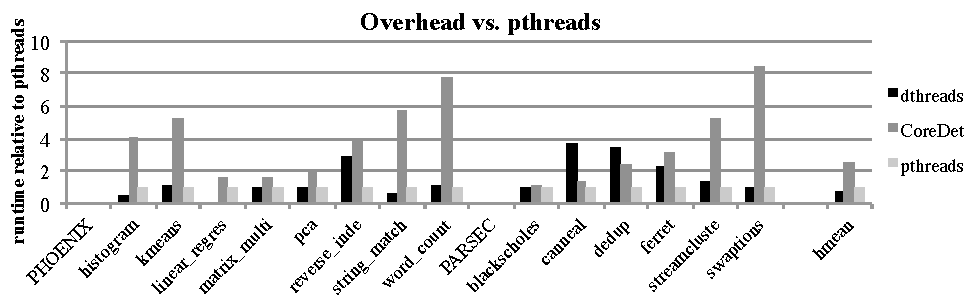
\includegraphics[width=6in]{dthreads/figure/overhead-figure}
\caption{Normalized execution time with respect to \pthreads{} and CoreDet(lower is better). For 9 of the 14 benchmarks, \dthreads{} runs nearly as fast or faster than \pthreads{}, while providing deterministic behavior.\label{fig:performance}}
}
\end{figure*}

\begin{table*}[!t]
\centering
\resizebox{\columnwidth}{!}{
\begin{tabular}{l|rrr|rr|l}
{\bf \small Benchmark} & {\bf \small CoreDet} & {\bf \small \dthreads{}} & {\bf \small \pthreads{}} & $\frac{\mbox{\bf \small CoreDet}}{\mbox{\bf \small \pthreads{}}}$ & $\frac{\mbox{\small \bf \dthreads{}}}{\mbox{\small \bf \pthreads{}}}$ & {\bf \small Input} \\

\hline
{\bf \small histogram} & 0.97 & 0.73 & 0.35 & $1.32\times$ & $0.48\times$ & {\it \small large.bmp} \\
{\bf \small kmeans} & 68.41 & 13.16 & 15.02 & $5.20\times$ & $1.14\times$ & {\it \small -d 3 -c 1000 -p 100000 -s 1000} \\ 
{\bf \small linear\_regression} & 6.42 & 4.11 & 0.57  & $1.56\times$ & $0.14\times$ & {\it \small key\_file\_500MB.txt} \\
{\bf \small matrix\_multiply} & 31.68 & 19.32 & 19.28  & $1.63\times$ & $0.99\times$ & {\it \small 2000 2000 } \\
{\bf \small pca} & 39.24 & 20.49 & 21.14  & $1.92\times$ & $1.03\times$ & {\it \small -r 4000 -c 4000 -s 100 } \\
{\bf \small reverse\_index} & 7.85 & 2.06 & 6.53 & $3.81\times$ & $3.17\times$ & {\it \small datafiles} \\
{\bf \small string\_match} & 18.31 & 3.19 & 1.97 & $5.74\times$ & $0.62\times$ & {\it \small key\_file\_500MB.txt} \\
{\bf \small word\_count} & 17.17 & 2.17 & 2.37 & $7.91\times$ & $1.09\times$ & {\it \small word\_100MB.txt} \\
{\bf \small blackscholes} & 10.49 & 9.47 & 9.30 & $1.11\times$ & $0.98\times$ & {\it \small 8 in\_1M.txt prices.txt} \\
{\bf \small canneal} & 14.74 & 10.41 & 39.82 & $1.42\times$ & $3.83\times$ &  {\it \small 7 15000 2000 400000.nets 128} \\
{\bf \small dedup} & 3.38 & 1.45 & 5.39 & $2.33\times$ & $3.72\times$ & {\it \small -c -p -f -t 2 -i media.dat output.txt} \\
{\bf \small ferret} & 21.89 & 7.02 & 26.86 & $3.11\times$ & $3.83\times$ & {\it \small corel lsh queries 10 20 1 output.txt} \\
{\bf \small streamcluster} & 14.33 & 2.74 & 4.61 & $5.23\times$ & $1.68\times$ &  {\it \small 10 20 128 16384 16384 1000 none output.txt 8} \\
{\bf \small swaptions} & 35.21 & 4.18 & 3.88 & $8.42\times$ & $0.93\times$ & {\it \small -ns 128 -sm 50000 -nt 8} \\
\hline
\end{tabular}
}
\caption{Benchmarks: execution time (in seconds) and input parameters.\label{tbl:benchmarks}}
\end{table*}

We next compare the performance of \dthreads{} to CoreDet
and \pthreads{}. Figure~\ref{fig:performance} presents these results graphically (normalized to \pthreads{}); Table~\ref{tbl:benchmarks} provides detailed information about execution time and input parameters.

\dthreads{} outperforms CoreDet on 12 out of 14 benchmarks (running between 20\% and $11.2\times$ faster). For 9 benchmarks, \dthreads{} runs nearly the same as or better
performance than \texttt{pthreads}. Because \dthreads{} isolates updates in separate processes, it can improve performance by eliminating false sharing: since concurrent ``threads'' actually execute in different physical pages, there is no coherence traffic caused by false sharing between synchronization points. \dthreads{} eliminates catastrophic false sharing in the \texttt{linear\_regression} benchmark, allowing it to execute over $7\times$ faster than \pthreads{} and $11\times$ faster than CoreDet. The \texttt{string\_match} benchmark exhibits a similar, though less dramatic, false sharing problem, allowing \dthreads{} to run almost 60\% faster than \pthreads{} and $9\times$ faster than CoreDet. Two benchmarks, \texttt{histogram} and \texttt{swaptions}, also run faster with \dthreads{} than with \pthreads{} ($2\times$ and $6\%$, respectively; $2.7\times$ and $9\times$ faster than with CoreDet). We believe but have not yet verified that the reason is false sharing.

For some benchmarks, \dthreads{} incurs modest overhead. For example, unlike most benchmarks examined here, which create long-lived threads, the \texttt{kmeans} benchmark creates and destroys over 1,000 threads in the course of its execution. 
While Linux processes are relatively lightweight, creating and exiting a process is still more expensive than the same operations of threads, accounting for a 14\% performance degradation of \dthreads{} over \pthreads{} (though it runs $4.6\times$ faster than CoreDet).

\dthreads{} runs substantially slower than \pthreads{} for 4 of the 14 benchmarks examined here. The \texttt{ferret} benchmark relies on an external library to analyze image files during the first stage in its pipelined execution model; this library makes intensive (and in the case of \dthreads{}, unnecessary) use of locks. Lock acquisition and release in \dthreads{} imposes higher overhead than ordinary \pthreads{} mutex operations. More importantly in this case, the intensive use of locks in one stage forces \dthreads{} to effectively serialize the other stages in the pipeline, which must repeatedly wait on these locks to enforce a deterministic lock acquisition order. The other three benchmarks (\texttt{canneal}, \texttt{dedup}, and \texttt{reverse\_index}) modify a large number of pages. With \dthreads{}, each page modification triggers a segmentation violation, a system call to change memory protection, the creation of a private copy of the page, and a subsequent copy into the shared space on commit (see Section~\ref{sec:future-work} for planned optimizations that may reduce this cost). We note that CoreDet also substantially degrades performance for these benchmarks, so much of this slowdown may be inherent to any deterministic runtime system.

\subsection{Scalability}
\label{sec:scalability}

\begin{figure}
{\centering
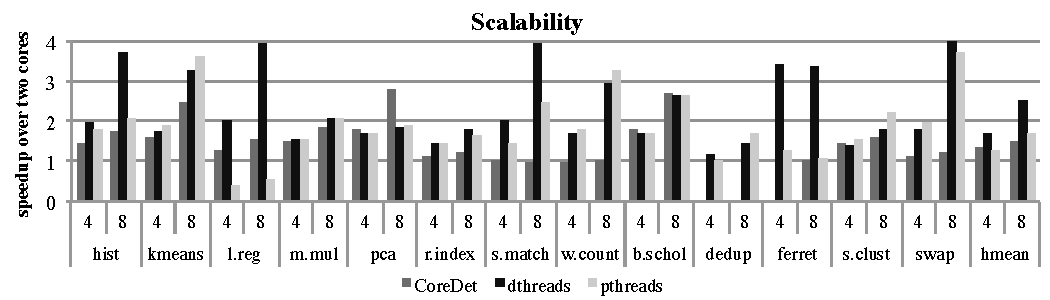
\includegraphics[width=6in]{dthreads/figure/scalability-figure}
\caption{Speedup of eight cores versus two cores (higher is better).  When possible to control with command line options, the number of threads was matched to the number of cores enabled.\label{fig:scalability}}
}
\end{figure}

To measure the scalability cost of running \dthreads{}, we ran two benchmark suite (excluding \texttt{canneal}) on the same machine with eight cores and again with two cores enabled.  Whenever possible without source code modifications, the number of threads was matched to the number of CPUs enabled.  We have found that \dthreads{} scales at least as well as \pthreads{} for 9 of 13 benchmarks, and scales as well or better than CoreDet for all but one benchmark where \dthreads{} outperforms CoreDet by 2x.  Detailed results of this experiment are presented in Figure~\ref{fig:scalability} and discussed below.

\texttt{canneal} was excluded from the scalability experiment because this benchmark does more work when more threads are present, making the performance comparison between eight and two threads unfair.  \dthreads{} hurts scalability relative to \pthreads{} for four of the benchmarks: \texttt{kmeans}, \texttt{word\_count}, \texttt{dedup}, and \texttt{streamcluster} although only marginally in most cases.  In all of these cases, \dthreads{} scales better than CoreDet.

\dthreads{} is able to match the scalability of \pthreads{} for three benchmarks: \texttt{matrix\_multiply}, \texttt{pca}, and \texttt{blackscholes}.  With \dthreads{}, scalability actually \emph{improves} over \pthreads{} for 6 out of 13 benchmarks: \texttt{histogram}, \texttt{linear\_regression}, \texttt{reverse\_index}, \texttt{string\_match}, \texttt{ferret}, and \texttt{swaptions}.




\subsection{Performance Analysis}

\subsubsection{Benchmark Characteristics}

The data presented in Table~\ref{tbl:characteristics} are obtained from the executions running on all 8 cores.  Column 2 shows the percentage of time spent in the serial phases.  In \dthreads{}, all memory commits and actual synchronization operations are performed in the serial phases.  The percentage of time spent in the serial phases thus can affect performance and scalability. Applications with higher overhead in \dthreads{} often spend a higher percentage of time in the
serial phases, primarily because they modify a large number of pages that need to be committed during those phases.

Column 3 shows the number of transactions in each application and Column 4 provides the average length of each transaction (ms).  Every synchronization, including locks, conditional variable, barriers, and thread exits, demarcate transaction boundaries in \dthreads{}.  For example, \texttt{reverse\_index}, \texttt{dedup}, \texttt{ferret}
and \texttt{streamcluster} perform numerous transactions whose
execution time is less than 1ms, imposing a performance penalty for these applications.  Benchmarks with longer (or fewer) transactions run almost the same speed as or faster than \texttt{pthreads}, including \texttt{histogram} or \texttt{pca}.  In \dthreads{}, longer transactions amortize the overhead of memory protection and copying.

Column 5 and 6 provides more detail on the costs associated with memory updates (the number and total volume of dirtied pages). From the table, it is clear why \texttt{canneal} (the most notable outlier) runs much slower with \dthreads{} than with \pthreads{}. This benchmark updates over three million pages, leading to large performance overhead caused by creating  private copies, handling protection faults, and committing modifications on those pages to the shared memory space. 

\textbf{Conclusion: }
Most benchmarks examined here contain either a small number of transactions, thus having long running transactions, and modify a modest number of pages during execution. For these applications, \dthreads{} is able to amortize its overhead: by eliminating false sharing, it can even run faster than \pthreads{}. However, for the few benchmarks that perform numerous short-lived transactions, or modify a large amount of pages, \dthreads{} can introduce substantial overhead.


\begin{table*}[!t]
\centering
\resizebox{\columnwidth}{!}{
\begin{tabular}{l|rrrrr}
& {\bf \small Serial Phase} & {\bf \small Transactions} & {\bf \small TransLength} & {\bf \small DirtyPages} & {\bf \small DirtyPages}
\\
{\bf \small Benchmark} & {\bf \small (\% of time)} & {\bf (\#)} & {\bf \small (ms)} & {\bf \small (\#)} & {\bf \small (GB)}\\
%\hline
%\multicolumn{6}{|c|}{\emph{Phoenix}} \\
\hline
\small \textbf{histogram} & 0 & 23 & 15.47 & 29 & 0 \\
\small \textbf{kmeans} & 0 & 3929 & 3.82 & 9466 & 0.04\\
\small \textbf{linear\_regression} & 0 & 24 & 23.92 & 17 & 0\\
\small \textbf{matrix\_multiply} & 0 & 24 & 841.2 & 3945 & 0.02\\
\small \textbf{pca} & 0 & 48 & 443 & 11471 & 0.04 \\
\small \textbf{reverseindex} & 17\% & 61009 & 1.04 & 451876 & 1.72\\
\small \textbf{string\_match} & 0 & 24 & 82 & 41 & 0 \\
\small \textbf{word\_count} & 1\% & 90 & 26.5 & 5261 & 0.02\\
%\hline
%\multicolumn{6}{|c|}{\emph{PARSEC}} \\
%\hline
\small \textbf{blackscholes} & 0 & 24 & 386.9 & 991 & 0\\
\small \textbf{canneal} & 26.4\% & 1062 & 43 & 3606413 & 13.75\\
\small \textbf{dedup} & 31\% & 45689 & 0.1 & 356589 & 1.36\\
\small \textbf{ferret} & 12.3\% & 484127 & 0.05 & 844184 & 3.21 \\
\small \textbf{streamcluster} & 18.4\% & 130001 & 0.04 & 131992 & 0.50\\
\small \textbf{swaptions} & 0 & 24 & 163 & 867 & 0\\
\hline
\end{tabular}
}
\caption{Benchmark characteristics.\label{tbl:characteristics}}
\end{table*}

\subsubsection{Performance Impact Analysis}
We further evaluate the performance impact of two important components of \dthreads: deterministic synchronization (sync-only) and memory protection(prot-only).

\emph{Sync-only}: This configuration enforces a deterministic synchronization order. However, the memory protection is not enabled so different processes access the shared memory directly. We want to use this to show the performance impact of load imbalance, caused by synchronization based scheduling.

\emph{Prot-only}: This configuration runs threads in isolation, with commits at synchronization points. The order of synchronization and memory commits are non-deterministic. This configuration eliminates false sharing, but also introduces the performance overhead of isolation and memory commits. In order to guarantee correct execution, we replaced those synchronizations as corresponding cross-processes synchronizations. The lazy twin creation and single-threaded execution optimizations are disabled here because they are unsafe without deterministic synchronization. Thus, this configuration actually evaluates the performance of using the \sheriff{} framework. 


\begin{figure*}[!t]
{\centering
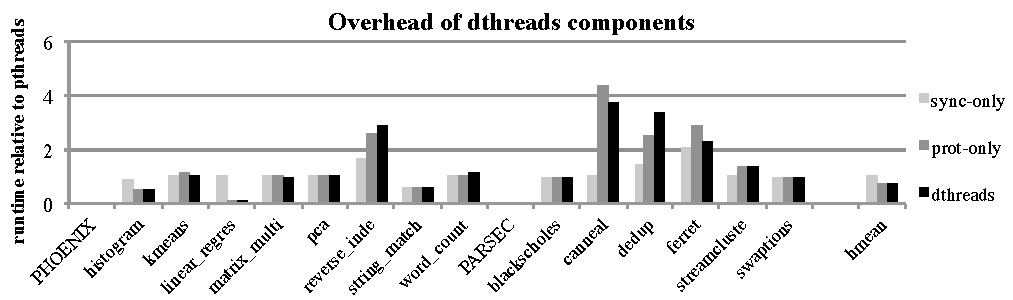
\includegraphics[width=6in]{dthreads/figure/perfeffect}
\caption{Normalized execution time with respect to \pthreads{} (lower is better) for three different configurations. 
\label{fig:perfanalysis}}
}
\end{figure*}

The performance results of these two configurations are shown in Figure~\ref{fig:perfanalysis} and discussed in the following.

\begin{itemize}

\item
The \texttt{reverse\_index}, \texttt{dedup} and \texttt{ferret} benchmarks show significant load imbalance under {\it sync-only} configuration. Additionally, these benchmarks introduces significant overhead with {\it prot-only} configuration because of a large number of transactions there. That explains why \dthreads{} doesn't have good performance on these benchmarks.

\item
The \texttt{string\_match} benchmark shows performance improvement with {\it sync-only} configuration. The exact reason is not clear, may be due to the per-thread allocator. 

\item
The \texttt{linear\_regression}, \texttt{histogram} and \texttt{swaptions} benchmarks improve performance with {\it prot-only} configuration. The memory isolation mechanism eliminates the false sharing problem inside and contributes to the performance speedup.

\item
Normally the performance of \dthreads{} is not better than the performance of {\it prot-only} configuration. However, both \texttt{ferret} and \texttt{canneal} run faster with determinism enabled. Both are benefited from specific optimization described in Section~\ref{sec:dthreads-optimization}. \texttt{ferret} benefits from the \emph{single-threaded-execution}. The performance improvement of \texttt{canneal} is coming from shared twin pages for all threads in the phase.

\end{itemize}








\chapter{Precise Detection and Automatic Mitigation of False Sharing}
\label{chapter:sherifftools}

Multithreading is an useful abstraction to exploit the hardware resources provided by a multi-core machine. Writing efficient multithreading programs remains challenging now. False sharing problem is one of notorious performance problem inside
multithreading programs. It occurs when multiple threads, running on different cores with separate caches, are accessing logically independent words in the same cache line. If a thread modify something inside a cache line, cache coherence protocol invalidates the duplicates of this cache line in other caches in order to guarantee a correct execution of a program, which is crucial for true sharing cases. However, it is totally unnecessary for false sharing cases. False sharing problem can force one core to wait unnecessarily for updates from another processor, thus waste both the CPU time and precious memory bandwidth in the same time. False sharing is a well-known performance issue~\cite{falseshare:Analysis, falseshare:effect}. 

Detecting false sharing requires tools support. All existing tools shared the same shortcoming, where they can not pinpoint the exact place with false sharing problems, leaving the burden of finding actual places to programmers. Besides that, existing tools suffer from one or more shortcomings.  Simulation based approaches ~\cite{falseshare:simulator} and binary instrumentation based approaches~\cite{falseshare:binaryinstrumentation1, falseshare:binaryinstrumentation2} normally introduce very significant performance overhead, slowing down the execution over $100\times$. Hardware performance counter based approaches generally provides much better performance, but they can not differentiate false sharing from true sharing problems~\cite{detect:ptu, detect:intel}.

We provide two tools to tackle with false sharing problem, based on the processes-as-threads framework - \sheriff{}. \SheriffDetect{} detects false sharing problem accurately (without false positives) and precisely, by pointing out the exact places with false sharing problems. Also, \SheriffDetect{} is very efficient, only introducing 20\% performance overhead. \Sheriff{} is a drop-in replacement library  of standard \pthreads{} library, which doesn't rely on advanced hardware support to find the problem.
We also provide a runtime system, \SheriffProtect{}, to automatically tolerate false sharing problems when rewriting an application to resolve false sharing is infeasible or impractical. The reason can be caused by either source is unavailable, or padding data structures would degrade performance because of reduced cache utilization and/or increase memory footprint.


%\section{\sheriff{} Framework}
%\label{sec:overview}

\begin{figure*}[!t]
\centering
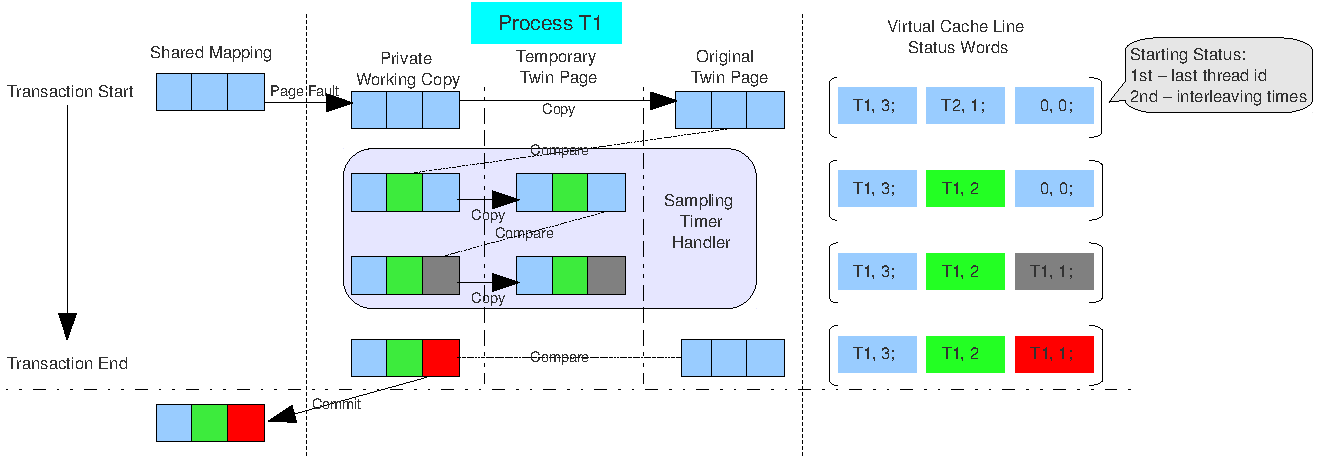
\includegraphics[height=2.3in]{sheriff/figure/overview.pdf}
\caption{
Overview about the execution of Sheriff(Section~\ref{simulation:thread}). 
Sheriff simuates threads using processes(Section~\ref{sec:simulation}). 
Each process works on its private copy  
and commits modifications of current process to shared mapping in the end of transaction(Section~\ref{simulation:endtran})
relying on ``twin page mechanism''(Section~\ref{overview-twinpage}) to get difference. 
To get interleaving writes for detecting false sharing, 
we introduce virtual cache line status words (Section~\ref{detection:invalidation}) 
and sampling mechanism(Section~\ref{detection:sampling}). 
No need for sampling mechanism and status words if only for a runtime system.
\label{fig:overview}}
\end{figure*}

Unlike previous tools, Sheriff is designed based on a completely different approach.
Sheriff doesn't rely on the hardware performance counter or binary instrumentation to find out false sharing problems. 
Alternatively, Sheriff tries to design a runtime system to simulate the running of multi-threaded program and 
monitor memory writes on different virtual cache lines from different threads.
%After the finding of cache lines with numerous interleaving writes,
Sheriff can precisely locate those objects or some fields inside objects causing serious performance problem. 

\subsection{Observations and Targets}
\label{overview:target}
There are two different types of false sharing problems according to 
the definitions of Hyde and Fleisch~\cite{falseshare:Analysis}. 
One is called as ``false sharing'' when multiple structurally unrelated objects 
are located in the same cache line. 
Another is called as ``pseduo sharing'' when multiple processors 
are accessing different fields of the same object.
Sheriff aims to find these two kinds of false sharing problems. 

Note that false sharing not always cause the performance problem. 
Whether one false sharing can cause performance problems depends on memory accessing pattern. 
We observe that false sharing can cause significant performance problems 
only when there are a lot of \textbf{interleaving} memory writes from different threads. 
Based on this observeration, Sheriff is trying to capture interleaving writes from different threads and 
report only those possible false sharing causing performance problem.
%%%%%%%%%%%%%%%%%%%%%%%%%%%%%%%%%%%%%%%%%%%%
%%%%% For global objects, Sheriff can tell the name of global objects which cause the false sharing problems.
%%%%% For heap objects, Sheriff can tell the callsite of malloc, thus programmer can 
%%%% refer to actual source code to find out which object caused the problems.
%%%%%%%%%%%%%%%%%%%%%%%%%%%%%%%%%%%%%%%%%%%%5
%Sheriff won't intend to find instructions that cause false sharing problems. Since multiple 
%instructions located in different functions can cause the same false sharing problem, but without the enough times 
%to capture the attention of programmer.
\begin{comment} 
There are two ways to tell false sharing problems. One is to tell users about the placement to 
touch those false sharing objects. Now PTU can point out functions to access specified addresses, without 
the name of false sharing objects, users should still try to figure out false sharing objects
in the whole function then they can decide how to fix the problem. 
Another is to tell users about false sharing objects, then user can find how false sharing happens.  
\end{comment} 
In order to reduce the manual overhead to locate the root of false sharing problems, Sheriff tries to indentify 
false sharing objects directly. 

Since Sheriff tries to replace those standard pthreads library (including memory allocator) 
in order to avoid the false positive problems 
caused by heap objects, Sheriff can not be used to detect those false sharing problems 
caused by memory allocator. 
We believe that is also reasonable since mordern memory allocator are trying to 
avoid false sharing problems as 
much as possible~\cite{BergerMcKinleyBlumofeWilson:ASPLOS2000}. 
%Section~\ref{effect-application} examplify the easiness to find the root of false sharing problem by using Sheriff.
\subsection{Assumptions}
\label{overview:assumption}
Sheriff has a basic assumption about those evaluating programs 
in order to simulate them correctly using multiprocess mechanism.
Those evaluated program are expected to no synchronization errors, 
such as deadlock, race condition or atomicity violations. 
We believe that this assumption is reasonable. 
If there are some synchronization problems inside, applications running using Sheriff
may have a higher probability to run uncorrectly, which can prevent Sheriff to find out all false sharing problems.

\subsection{Process as Threads}
One basic mechanism of Sheriff is to treat threads as processes, which is used firstly by Grace~\cite{grace}.
%But Sheriff discards the sequential semantics of Grace, which Grace tends to use that to avoid concurrency errors. 
%Also, Sheriff discards the limit of Grace (no synchronization inside) and try to provide a framework
%which can work on general multi-threaded programs. 
Process has its own address space and signal handler table, provides strong isolation between different threads, 
which makes it perfect for Sheriff
to monitor memory accesses from different threads.
More importantly, we can utilize process to eleminate false sharing inside, no need
to let other threads to know results if no explicit synchronization.

There is a natural concern about the performance to use process instead of threads.
Although the overhead to create and exit one process is       
much more than that for one thread, we don't need pay too much overhead here since  
thread's creation and exit won't happen frequently and normal execuation of Sheriff 
can be almost the same speed as that of processes.

Section~\ref{sec:simulation} gives more details about how to simulate threads using process.
\subsection{Twin Page Mechanism}
\label{overview-twinpage}
Sheriff can capture those pages modified by one process 
when one process are trying to write on those pages protected as read-only mode.
But it is clear that page granularity is too coarse to locate cache false sharing problems.  
To avoid this problem, Sheriff are trying to use twin page mechanism to find the modifications on words. 
Twin page mechanism was first used in Munin~\cite{dsm:treadmarks} to 
capture modifications on a page in distributed share memory system.

The mechanism 
can be seen in Fig.~\ref{fig:overview}. 
Before one working page is modified, a ``twin page'' is created which is indentical
to the working page which are going to be modified. The twin page is keeping intact when the working
page are modfied. 
Later, the twin page and the working page can be compared byte by byte
later in order to capture those modifications made on the working page.
\begin{comment}
In the beginning of one synchronization phase, all pages are protected. 
At the first write on one protected page,
a page protection violation occurs. 
Operating system should send a signal handler to current process causing protection violation, 
then in the signal handler Sheriff can makes a copy of current page (creation of a twin page) 
and removes the protection on this page so that future 
writesi (in the same phase) on this page can run at a full speed. 
The twin page and the working copy of current process can be compared word by word
later to capture those writes on this page in one phase.
\end{comment}
More details about using the ``twin page mechanism'' can be seen in Section~\ref{sec:falseshare}.
%In this meaning, we are trying to introduce the "twin" mechanism used in DSM system in a general multithreaded
%program by leveraging constructively the process mechanism in the same time. 


\section{Detecting False Sharing}
\label{sec:falseshare}
From above section, we already know that how to design a runtime system to simulate the running 
of multi-threaded program. 

In this section, we are going to talk how to indentify false sharing problems by recording memory writing using
the runtime system.
This section are trying to answer the following questions:

\begin{itemize}
\item How to capture the memory writes from different process?
\item How to capture the continuous memory writes?
% - sampling mechanism - "temporary twin" and "original twin". 
\item How to capture the interleaving cache invalidation? 
% Use a global array, updating timely when modification is detected. 
\item How to identify objects inside one cache line? 
%Attach the callsite information to capture the allocate sites for heap objects. 
\item How to differentiate true sharing and false sharing?
%detect the combination? An array to get word version and threads working on that. We can detect those fields inside one object causing the problem too.
\item How to report one false sharing problem?
% In the end of program, we traverse the whole global array.
\end{itemize}

\subsection{Capture of Memory Writes}
\label{falseshare:memorywrites}
Process can provide a strong isolation of one thread's running from other threads' running. 
In each transaction, Sheriff runs one thread in a atomical, consistent and isolated way and
won't commit those changes in one transaction until the end of one transaction.
In the end of each transaction, Sheriff can compare ``twin'' page and ``working'' page word by word to find 
those modifications on each dirty page. When the word of ``working'' page is different from that of 
corresponding ``twin'' page, this word is thought to be modified by current thread in current transaction. 
It is reasonable to reach this conclusion since Sheriff can guarantee that originally the content of ``twin'' page 
is the same as that of ``working'' page by forcing a COW explicitely (see ~\ref{simulation:execution}).
\begin{comment}
It is true that the writing of ``A-B-A''  can be missed by simply comparison,
but we believe that ``A-B-A'' writing in one transaction
is not frequent and won't bring any correctness problem.
We don't want to put too much focus on this point.
\end{comment}

Since we can capture the memory writes on every transaction and one thread's running is consisted of multiple transactions, 
we can capture the memory writes from different threads.

\subsection{Capture of Continuous Writes}
\label{detection:sampling}
We already know from above section that Sheriff can capture memory writes on one transaction. 
But it is not good enough when the transaction length is too long (some extreme case can be the whole thread). 
Actually, one serious false sharing problem (\texttt{linear\_regression} benchmark, see Section~\ref{sec:evaluation}) 
which affect the performance 10X can be omitted since there is only one transaction for one thread, 
without any synchronization inside. 

Sheriff use a sampling mechanism to avoid this problem. Sampling is 
to select some of observations in order to acquire some knowledge about the whole.
Although sampling cannot give complete information about memory writes on one transaction,
sampling can be used to capture more writes. More fine sampling can help to find more writes by one transaction.
There is a balance between choosing finer sampling period and performance issue here. 
Sheriff now choose 10 microseconds as a basic interval to do sampling. 

In order to capture continuous writes, Sheriff introduce one ``temporary twin'' page for every shared dirty page
 (see Fig.\ref{fig:overview}). 
Handling of those ``temporary twin'' pages are slightly diferent with those ``original twin'' pages.
First, they are created in the sampling timer handler when one page is found to be shared by multiple threads. 
There is no use to create ``temporary twin'' for those pages only accessed by one thread. We are using a global array to
record users for one page. 
Second, ``temporary twin'' pages are keeping updated to ``working'' version in every timer handler 
in order to capture future writes on the same page.
 
\subsection{Capture of Cache Invalidations}
\label{detection:invalidation}
Just as we talked in Section~\ref{overview:target}, only numerous interleaving writes can bring performance problem. 
Sheriff tries to capture the interleaving writes across different threads in order to capture 
cache invalidations. 

In order to capture interleaving writes on caches, Sheriff introduces 
virtual cache line status words (Fig.~\ref{fig:overview}). 
``virtual'' is used here to differentiate with ``physical'' cache line. 
For every virtual address range (same size with physical cache line) under protection, Sheriff assigns one status word. 
One status word has two fields, the first field points last thread to write on this cache line, 
the second field is used to record times of invalidates (version) on one cache line. 
Every time when one different thread are detected to write on this cache line, Sheriff update both the thread id
to be the new thread and version number. 
In actual implementation, Sheriff introduce two different arrays to avoid using lock. Corresponding code can be seen
in Figure~\ref{fig:capturecacheinvalidation}.
CacheInvalidation array is used to capture those interleaving cache invalidation for all cache lines in protected memory. 
Every cache line have one corresponding counter to indicate the interleaving of cache invalidation for this cache line. 
LastThreadModifyCache array is used to record last thread id to write on its cache line. 

The pseudo code to capture the interleaving cache invalidation is listed in Figure~\ref{fig:capturecacheinvalidation}:
\begin{figure*}[!t]
\begin{lstlisting}
void recordCacheInvalidates(int cacheNo) {
    int myTid = getpid();
    int lastTid;

    // Try to check last thread to modify this cache.
    lastTid = atomic_exchange(&LastThreadModifyCache[cacheNo], myTid);
    if(lastTid != myTid) {
       // Increment cache invalidation only when current thread is different.
       atomic_increment(&cacheInvalidation[cacheNo]);
     }
}
\end{lstlisting}
\caption{Record the cache invalidation atomically.\label{fig:capturecacheinvalidation}}
\end{figure*}

\subsection{Indentify Objects inside Cache Line}
\label{detection:object}
For global object, Sheriff don't need to do anything since debug information can provide
object's information.
Sheriff attaches the call site in the header of each heap object when allocation to indentify objects.
Callsite information can provide objects' request allocation, which is useful for programmer
to fix the false sharing problem (see case study in Section~\ref{evaluation:comparison}).
It is one important feature to differentiate Sheriff from previous tools.
Previous tools using binary instrumentation or hardware performance counter cannot control
the memory allocation, so they cannot provide the callsite information about one object.
Sheriff is a runtime system which intercepts all heap allocations so that Sheriff can tell programmer
about cache line's object information.

Remember that Sheriff have two arrays to capture the cache interleaving invalidation
(see Section~\ref{detection:invalidation}), it is necessary to cleanup those invalid counting
when one object is de-allocated. It is important to avoid the false positives caused by uncorrectly aggregate 
counting when one address is re-used for other objects. 

\subsection{Avoidance of False Positives}
\label{detection:avoidfalsepositive}
To avoid false positives, 
Sheriff introduces another global array to record  
threads writing on each word and version numbers of each word.
Threads writing on each word can tell whether one cache line is false sharing or true sharing. 
Version number on each word can avoid to report those objects which don't contribute much on cache invalidations, 
when there are multiple objects in the same cache line.
In order to save space, Sheriff use one word's higher 16 bit to store the thread id on one word
and use the lower 16 bit to store version number of this word. 
When one word is detected to be modified by more than two threads, we marked specially
on its thread id field.

\subsection{Reporting False Sharing Objects}
In the end of program, Sheriff reports those objects causing false sharing problems. 
Since Sheriff introduce a global array (CacheInvalidationArray) to record those 
cache invalidation (see Section~\ref{detection:invalidation}), Sheriff checks 
CacheInvalidationArray for cache lines with invalidation times larger than one water level. 
After one cache line is found, corresponding invalidation times and offset of this cache line 
will be added into a global link linst sorted by invalidation times. 
Later we can rank the false sharing objects by invalidation times they caused. 

After the traverse of all cache lines, Sheriff tries to get objects information 
for all cache lines in the link list. 
Sheriff uses magic value added in the allocation to differentiate the start of one object. 
Also, the object size information can help to identify the start of one object. 
After finding out those objects inside one cache line, Sheriff should look into the 
array listed in Section~\ref{detection:avoidfalsepositive} to avoid false positives. 

%%%%%%%%%%%%%%%%%%%%%%%%%%%%%%%%%%%%%%%%%%%%%%%%%%%%%%%%%%%%%%%%%%%%%%%%%%%%%
%%%%%%%%%%%%%%%% Where to specify those procedure of timer handler????? LTP
%%%%%%%%%%%%%%%%%%%%%%%%%%%%%%%%%%%%%%%%%%%%%%%%%%%%%%%%%%%%%%%%%%%%%%%


\section{Tolerating False Sharing}
\label{sec:sheriffprotect}
While \SheriffDetect{} can effectively find those false sharing problems of multithreaded programs, it is sometimes difficult or impossible to fix them in order to boost the performance. For example, padding memory to avoid false sharing may even slowdown the performance because of excessive memory consumption or reducing cache utilization~\cite{qinzhao}. Also, time constraints or unavailable source code may prevent the fixes. 

Based on the \sheriff{} framework, we provide the second tool, \SheriffProtect{}, to automatically boost the performance for multithreaded applications with false sharing problems, without programmer intervention.  

\SheriffProtect{} borrows the insight initially introduced by Dubois et.al.~\cite{Dubois:1991:DCE:125826.125941}: {\it delaying updates avoids false sharing}. Because \Sheriff{} replaces threads with processes, executions of different threads are actually isolated from each other. Thus, different ``threads'' (processes) actually access different physical cache lines, when originally they are accessing the same cache line in the multithreading environment. This helps avoid false sharing problems. 

However, simply using \sheriff{} may introduce excessive performance overhead because of the following reasons: 

\begin{itemize}
\item
The overhead of protecting and committing all pages may be too high. As we already know in Section~\ref{sec:sheriffframework}, \sheriff{} has to commit all local changes of different threads  to the shared mapping at the end of every transaction (synchronization points) in order to achieve the shared memory semantics. 

\item
If the length of a transaction is short, the overhead of protecting and committing pages in \sheriff{} can be easily higher than the performance benefit by tolerating possible false sharing problems inside. Thus, there is no benefit to tolerate false sharing problems for short-running transactions. 

\end{itemize}

\sheriffprotect{} provides two corresponding mechanisms to avoid these possible overhead. 

\emph{Selective Protection.} 
\SheriffProtect{} only prevents false sharing on small objects (those less than 1024 bytes in size). All large objects are mapped shared and are never protected, thus can not tolerate false sharing problems caused by these large objects. We expect  small objects to be a likely source of false sharing because more of them can fit on a cache line. Also, for large objects, the cost of protecting and committing changes can be bigger than the benefit of tolerating possible false sharing problems inside. 

\emph{Adaptive Prevention.}
\SheriffProtect{} employs a simple adaptive mechanism: it only isolates threads' executions if the average transaction length is large than a pre-set threshold. \SheriffProtect{} keeps track of the length of each transaction and uses exponential a weighted averaging ($\alpha = 0.9$) to calculate the average transaction length. If the average transaction length falls below an established threshold, \SheriffProtect{} switches to shared mappings for all memory and does no further page protections. As long as transactions remain too short, 
 without any benefit to tolerate false sharing problems inside, the protection mechanisms remain switched off. If the average transaction length rises back above the threshold, \SheriffProtect{} re-establishes private mappings and page protections, thus avoiding possible false sharing to achieve better performance.

\section{Experimental Evaluation}
\label{sec:evaluation}

We perform our evaluations on a quiescent 8-core system (dual
processor with 4 cores), with 8GB of RAM. Each processor is a 4-core 64-bit Intel Xeon, running at 2.33 Ghz with a 4MB L2 cache. For compatibility reasons, we compiled all applications to a 32-bit target using GCC. All performance data is the average of 10 runs, excluding the maximum and minimum values.

The evaluation answers the following questions:

\begin{itemize}
\item How effective is \sheriffdetect{} at finding false sharing and guiding programmers to their resolution? (Section~\ref{sec:effecteval})
\item What is \sheriffdetect{}'s performance overhead? (Section~\ref{})
\item How sensitive is \sheriffdetect{} to different sampling rate? (Section~\ref{}) 
\item How effective does \sheriffprotect{} mitigate false sharing? (Section~\ref{})
\end{itemize}

\subsection{\sheriffdetect{} Effectiveness}

\label{sec:effecteval}

This section evaluates whether \sheriffdetect{} can be used to find false sharing problems, both in synthetic test cases and in actual applications.

We developed a range of microbenchmarks that exemplify different situations related to false sharing. We evaluate these benchmarks on both \SheriffDetect{} and Intel's Performance Tuning Utility(PTU v3.2), the previous state-of-the-art work of false sharing detection.
Detection results are shown in Table~\ref{table:microbenchmarks}. \sheriffdetect{} only reports those false sharing instances that can possibly affect the performance, while correctly ignores those cases without no performance impact.
PTU has false alarms/positives.  It does not track those pattern of accesses, which reports false positives for those non-interleaved accesses. Also, PTU does not track memory deallocations, thus it can not filter out those pseudo false sharing caused by memory reuse. \sheriffdetect{} avoids all of these problems and reports false sharing problems correctly. 


\begin{table}
\centering
\begin{tabular}{l|l|l|l}
\hline
{\bf \small Microbenchmark} & {\bf \small Perf Sensitive } & {\bf \small \sheriffdetect{} } & {\bf \small PTU } \\
\hline

\small \textbf{False Sharing (adjacent objects)} & YES & \cmark{} & \cmark{} \\
\small \textbf{False Sharing (same object)} & YES & \cmark{} & \cmark{} \\
\hline
\small \textbf{True Sharing} & NO & & \\
\small \textbf{Non-interleaved False Sharing} & NO & & \xmark{}\\
\small \textbf{Heap Reuse(no sharing)} & NO & & \xmark{}\\
\hline
\end{tabular}
\caption{False sharing detection results using PTU and \sheriffdetect{}. \sheriffdetect{} correctly reports only actual false sharing instances, with a performance impact;
\cmark{} indicates a correct report and \xmark{} indicates a false alarm. 
\label{table:microbenchmarks}}
\end{table}

We further evaluate \SheriffDetect{} and PTU on two widely-used benchmarks suites, Phoenix~\cite{phoenix-hpca} and PARSEC~\cite{parsec}. We use the simlarge inputs for all applications of PARSEC. For Phoenix, we chose available parameters that allow the programs to run as long as possible. As of this writing, we were unable to successfully
compile \texttt{raytrace} and \texttt{vips}, and \sheriff{} is
currently unable to run \texttt{x264}, \texttt{bodytrack},
and \texttt{facesim}. Freqine currently can not support pthreads. Thus, those benchmarks are excluded here. 
 
\begin{table}
\centering
\begin{tabular}{l|r|r}
\hline
{\bf \small Benchmark} & {\bf \small PTU} & {\bf \small \sheriffdetect{}}\\
 & {\# Lines} & {\# Objects}\\
\hline
\small \textbf{kmeans} & 1916 &  2 \\
\small \textbf{linear\_regression} & 5 & 1 \\
\small \textbf{matrix\_multiply} & 468 & 0\\
\small \textbf{pca} & 45 & 0 \\
\small \textbf{reverseindex} & N/A & 5 \\
\small \textbf{word\_count} & 4 & 3\\
\hline
\small \textbf{canneal} & 1 & 1 \\
\small \textbf{fluidanimate} & 3 & 1 \\
\small \textbf{streamcluster} & 9 & 1\\
\small \textbf{swaptions} & 196 & 0\\
\hline
\small \textbf{Total} & 2647 & 14\\
\hline
\end{tabular}
\caption{Overall detection results of PTU and \sheriffdetect{} on Phoenix and PARSEC benchmark suites. We only list those benchmarks that at least one of tools reports false sharing problems. For PTU, we show how many cache lines are marked as falsely shared. For \sheriffdetect{}, we show how many objects are reported by \sheriffdetect{} (with cache invalidations larger than 100). The item marked as ``N/A'' means PTU fails to show results because it runs out of memory.
\label{table:fsdetection}}
\end{table}


The overall results are shown in Table~\ref{table:fsdetection}. PTU reports that 2647 cache lines may exist false sharing problems, given that they can report false positives. \sheriffdetect{} reveals that seven out of sixteen evaluated benchmarks have some false sharing issues. Totally, only 14 objects are reported, but only 4 of them shows a big number of cache invalidations. 

Several reasons contributes to this big difference. First, PTU reports cache lines information about false sharing objects, while \SheriffDetect{} only reports objects. Second, PTU reports multiple times if a heap object, with the same allocation site, is allocated multiple times. 
Third, PTU may report false positives since it do not track interleaved accesses and overrate the problems caused by heap reuses. 


We manually fix these four false sharing problems based on reports of \SheriffDetect{}, and showed the performance data in Table~\ref{table:perfafterfix}. To explain why performance improvement are different, we examine the maximum possible updates occurred on these false sharing objects, the reason of performance improvement. For example, \texttt{linear\_regression} has the largest updates, thus causes serious performance problem because of false sharing. 

\begin{table}
\centering
\begin{tabular}{l|r|r}
\hline
{\bf \small Benchmark} & {\bf \small Performance Improvement} & {\bf \small Updates}\\
 & & (M)\\
\hline
\small \textbf{linear\_regression} & 818\% & 1323.6\\
\small \textbf{reverseindex} &  2.4\% & 0.4\\
\small \textbf{streamcluster} & 5.4\% & 28.7\\
\small \textbf{word\_count} &  1\% & 0.3\\
\hline
\end{tabular}
\caption{Performance data for four false sharing benchmarks. 
All data are obtained using the standard \pthreads{} library. 
``Updates'' shows how many million updates (in total) occurred on falsely-shared cache lines.
\label{table:perfafterfix}}
\end{table}


In \texttt{reverse\_index} and \texttt{word\_count}, multiple threads repeatedly modify the same heap object. The pseudo code for these two benchmarks are listed in Figure~\ref{fig:reverseindex}. We may use thread-local copy to avoid the false sharing problem here; each thread can modify a temporary variable first and then modify the global \texttt{use\_len} in the end of thread.

\begin{figure}[!t]
\begin{lstlisting}
int * use_len;
void insert_sorted(int curr_thread) {
   ......	
   // After finding a new link
   (use_len[curr_thread])++;
   ......	
}
\end{lstlisting}
\caption{A fragment of source code from \texttt{reverse\_index}. False sharing arises when adjacent threads 
modify the \texttt{use\_len} array. 
\label{fig:reverseindex}}
\end{figure}

\texttt{Linear\_regression}'s false sharing problem is a little different (see Figure~\ref{fig:linear_regression}). 
Two different threads write to the same cache line when the
structure \texttt{lreg\_args} is not cache line aligned. This problem can be avoided easily by padding the structure \texttt{lreg\_args}.

\begin{figure}[!t]
\begin{lstlisting}
struct {
  long long SX;
  long long SY;
  long long SXX;
  ......
} lreg_args;

void *lreg_thread(void *args_in) {
  struct lreg_args * args = args_in;
  for(i = 0; i < args->num_elems; i++) {
    args->SX  += args->points[i].x;
    args->SXX += args->points[i].x 
   	         * args->points[i].x;
  }
  ......	
}
\end{lstlisting}
\caption{A fragment from \texttt{linear\_regression} code. 
Each thread is passed in a different address (\texttt{struct lreg\_args}) and each thread can work on its corresponding \texttt{args\_in}. 
Unfortunately, the size of \texttt{struct lreg\_args} is not cache line aligned (52 bytes) and that
causes two different threads to write to the same cache line simultaneously. 
\label{fig:linear_regression}}
\end{figure}

The false sharing problem detected in \texttt{streamcluster} (one of the PARSEC benchmarks) is similar to the false sharing problem in \texttt{linear\_regression}; two different threads are writing on the same cache line.  In fact, the author tried to avoid the false sharing problems and make every stride a multiple times of cache line size. But the default cache line size is 32 bytes, which is different from the actual physical cache line size that we are used in evaluation (64 bytes).  By simply setting the \texttt{CACHE\_LINE} macro to 64 bytes, it is possible to avoid this false sharing problem completely.


\subsection{Ease of locating false sharing problems}

\noindent
To illustrate how \sheriffdetect{} can precisely locate false sharing problems, we 
use one benchmark (\texttt{word\_count}, a PHOENIX benchmark) as
an example. Our experience with diagnosing other false sharing issues is similar.

Here is an example output from \sheriffdetect{} from \texttt{word\_count}.

\begin{verbatim} 
1st object, cache interleaving writes 
13767 times (start at 0xd5c8e140). 
Object start 0xd5c8e160, length 32. 
It is a heap object with callsite:
callsite0:./wordcount_pthreads.c:136
callsite1:./wordcount_pthreads.c:441
\end{verbatim}

Line 136 (\texttt{wordcount\_\pthreads{}.c}), 
contains the following memory allocation call:

\begin{verbatim}
use_len=malloc(num_procs*sizeof(int));
\end{verbatim}

Grepping for \texttt{use\_len}, a global pointer, quickly leads to this line:

\begin{verbatim}
use_len[thread_num]++;
\end{verbatim}

Now it is clear that different threads are modifying the same object
(use\_len). Fixing the problem by using the
thread-local data copies is now straightforward~\cite{detect:intel}.

By contrast, compare PTU's output in Figure~\ref{fig:wordcount}. Finding this problem is far more complicated with PTU, since it only presents functions using each cache line, not to mention the fact that PTU can
report huge numbers of false positives.  Another shortcoming
of PTU is that ``Collected Data Refs'' number cannot be used as a metric to evaluate the significance of false sharing problems. For this example, PTU only reports 12 references (versus 13767 times for \sheriffdetect{}).

\begin{figure*}[!t]
\centering
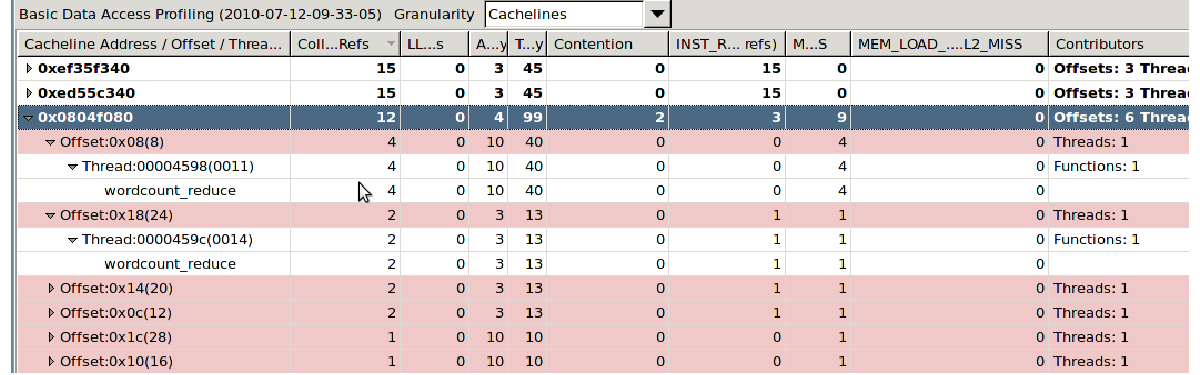
\includegraphics[width=6in]{sheriff/figure/wordcount}
\caption{PTU output for \texttt{word\_count}.
\label{fig:wordcount}}
\end{figure*}

%That is why we cannot relying on PTU to do the analysis of false sharing
%problems given the large number of cache lines involved. 

\subsection{\sheriffdetect{} Performance Overhead}
\label{sec:results-runtime-overhead}

\begin{figure*}[!t]
\centering
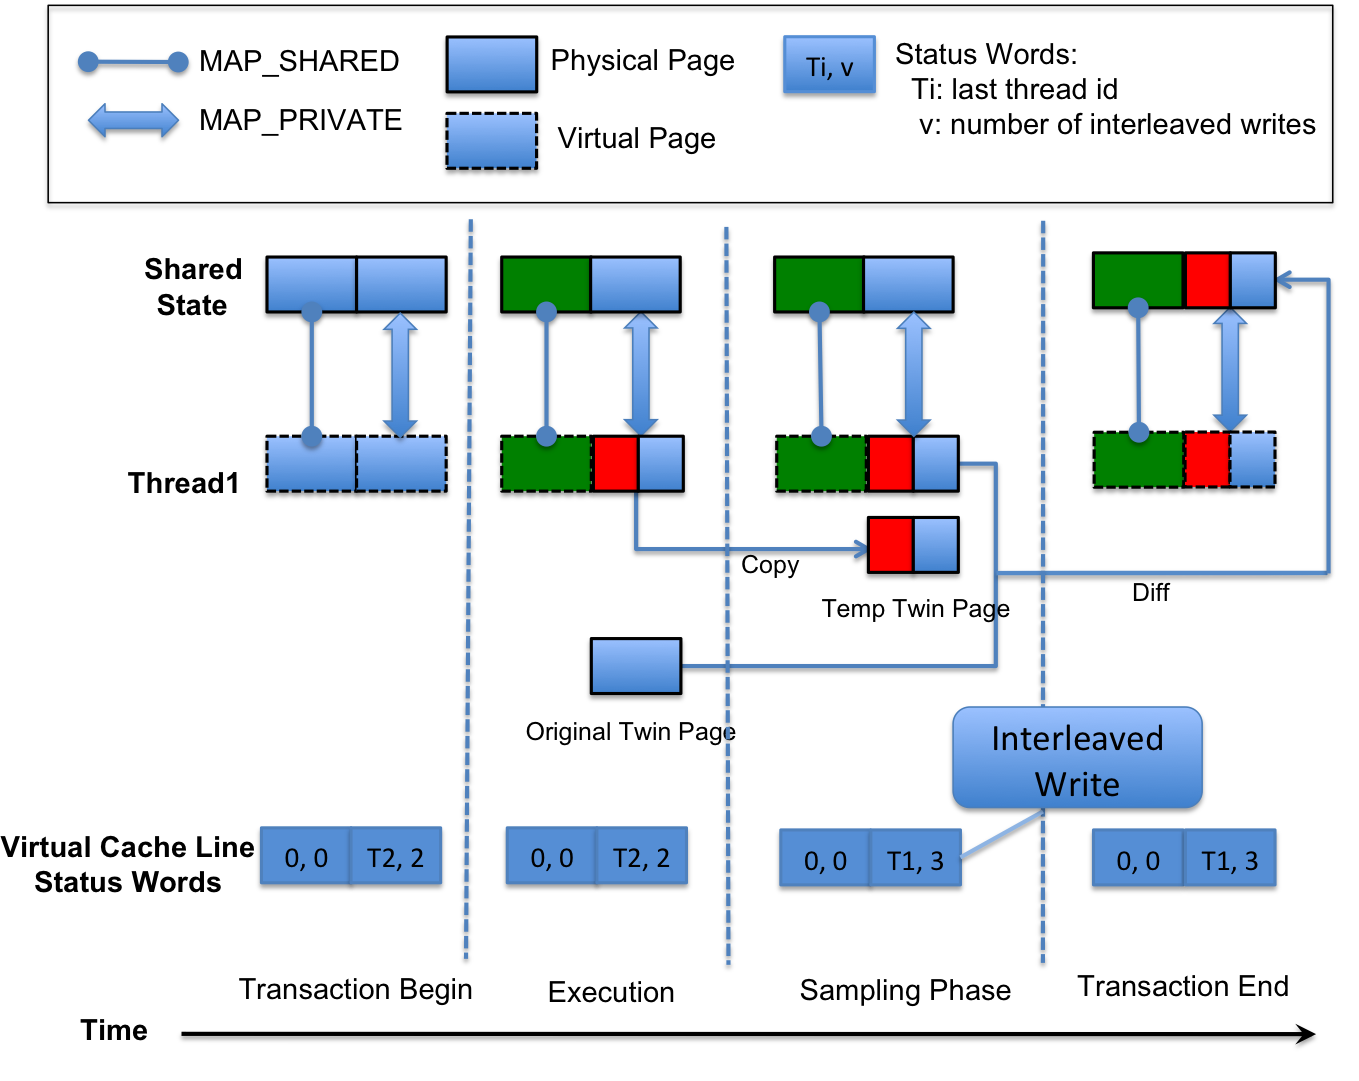
\includegraphics[width=6in]{sheriff/figure/detective.png}
\caption{\sheriffdetect{} overhead across two suites of benchmarks,
  normalized to the performance of the \pthreads{} library (lower is better). 
  With two exceptions, its overhead is acceptably low.
\label{fig:overhead}}
\end{figure*}


This section shows the runtime overhead of \sheriffdetect{} (comparing to \pthreads{})on
two multithreaded benchmarks suites, PHOENIX and PARSEC.  The results
can be seen from Figure~\ref{fig:overhead}.  

\texttt{linear\_regression} exhibits almost
a 10X speedup against the one using \pthreads{} library even with the added overhead of sampling and 
other mechanisms of \sheriffdetect{}.  There is a
serious false sharing problem inside (see
Table~\ref{table:perfafterfix}) which both \sheriffdetect{} and \sheriffprotect{} eliminate
automatically. 

There are two benchmarks on which \sheriffdetect{} do not perform well. 
One is \texttt{canneal}, the performance overhead of \sheriffdetect{}
on this benchmark is about 7X slower than the one using \pthreads{}
library. Another one is \texttt{fluidanimate}, the performance overhead is about 
14X slower than that using \pthreads{}.

According to our analysis, the transaction number and dirty pages are two main causes 
of the overhead. For most of time, more transaction number can cause more dirty pages.  
In order to find out what can affect the performance of these two benchmarks, 
we get some characteristics data(see Table~\ref{tbl:characteristics} about these 
two benchmarks when they are using 
the \sheriffdetect{}.

\begin{table}
\centering
\begin{tabular}{|l|r|r|r|}
\hline
{\bf \small Benchmark} & {\bf \small Trans} &{\bf \small DirtyPages} & {\bf \small Runtime} \\
 & {\#} & {M} & {s}\\
\hline
{\bf \small canneal} & 930 & 2.9 & 74.3 \\
{\bf \small fluidanimate} & 18696114 & 2.15 & 21.56\\
\hline
\end{tabular}
\caption{Characteristics of slower benchmarks in \sheriffdetect{}.
\label{table:characteristics}}
\end{table}

From the table, we can easily find out that these two benchmarks share the same attribute, having large amount of dirty pages. 
For one dirty page, \sheriffdetect{} need two protections, creation of the Copy-On-Write version and
different version of twin pages, checking the false sharing problem inside every periodical checking cycle and 
commits to the shared mapping. Given large amount of dirty pages, copying alone is very expensive 
since one dirty page needs at least 3 copies. 
For \texttt{fluidanimate}, 2.2 million pages needs about 6.8 million copies, which can 
acount for about 20 seconds copying overhead since copying one gigabyte of memory takes approximates 0.75 seconds.
shared pages, which leads to substantial overhead.
Examination of the source code of \texttt{fluidanimate} reveals a large number of lock
calls, \sheriff{} replaces lock calls with their interprocess variants
and triggers a transaction end and begin for each, adding some overhead if there are some shared pages.
 
\begin{comment}
The worst case for \sheriff{} is exemplified
by \texttt{ferret}, which modifies a huge number of pages (about
3.45G) and has a large number of transactions (about 1M).
We also measured charecteristics of our benchmark suites in
Table~\ref{table:characteristics}.  The
following parameters determine the performance of \sheriff{}.

\begin{itemize}
\item
Pages written: each write on a protected page imposes
additional overhead to unprotect the page in the page fault handler.
In the sampling handler, \sheriff{} must check for cache writes for
each shared written page, and at the end of transaction, \sheriff{} must
check cache writes for each page and commit the modification to the shared
space.

\item
Transaction length: \sheriff{} introduces overhead in the beginning
of transaction and in the end of each transaction. Longer transactions
amortizes this overhead.

\item 
Allocation times: \sheriff{} (in detection mode) attaches callsite information for every
allocated object, slowing allocation.

\item
Cache cleanup size: \sheriff{} cleans up the invalid cache counting
information in the memory allocation if one allocation is involving in
the re-usage of memory of those freed memory objects.
\end{itemize}

From the results from Table~\ref{table:characteristics}, we can
confirm our analysis.  Allocation times and cache cleanup size have
little impact on performance. However, when the number and rate of
pages written is large, performance suffers.

Figure~\ref{fig:overhead} shows that \sheriff{}'s overhead is highest for
the following two benchmarks: \texttt{fluidanimate} and \texttt{canneal}.
For \textt{canneal}, different threads are writting to a lot of shared pages
benchmarks \texttt{ferret}, \texttt{reverse\_index}, \texttt{dedup}
and \texttt{fluidanimate}. Characteristics showed in
Table~\ref{table:characteristics} that the first three benchmarks have
a very high rate of page updates (\textbf{PagesPerMs}). 
\texttt{fluidanimate} is an outlier if we are just using the \textbf{PagesPerMs} metrics.
The reason of \texttt{fluidanimate} has a high overhead is that there
are huge amounts of transactions inside (about 10M). Examination of
the source code revealed a large number of lock calls in this
application. \sheriff{} replaces lock calls with their interprocess
variants and triggers a transaction end and begin for each, adding
overhead.  The worst case for \sheriff{} is exemplified
by \texttt{ferret}, which modifies a huge number of pages (about
3.45G) and has a large number of transactions (about 1M).

\begin{table*}
\centering
\begin{tabular}{|l|rrrr|rr|r|}
\hline
{\bf \small Benchmark} & {\bf \small PagesWritten} & {\bf \small Commits} & {\bf Allocs} & {\bf \small CleanupSize} & {\bf \small TranLength(ms)} & {\bf \small PagesPerTran} & {\bf \small PagesPerMs}\\
\hline
\small \textbf{histogram} & 0 & 24 & 2 & 0 & 12.5 & 0 & 0\\
\small \textbf{kmeans} & 1312 & 3836 & 101002 & 0 & 4.15 & 0.34 & 0.08\\
\small \textbf{linear\_regression} & 16 & 24 & 3 & 0 & 38.6 & 0.67 & 0.02\\
\small \textbf{matrix\_multiply} & 16 & 24 & 11 & 0 & 313.23 & 0.67 & 0.0\\
\small \textbf{pca} & 0 & 47 & 2 & 0 & 450.69 & 0 & 0.0\\
\small \textbf{reverseindex} & 260201 & 156409 & 250927 & 0 & 0.05 & 1.66 & 30.99 \\
\small \textbf{string\_match} & 0 & 24 & 7 & 0 & 104.75 & 0 & 0.00\\
\small \textbf{word\_count} & 145 & 89 & 38 & 32 & 25.08 & 1.63 & 0.06\\
\hline
\small \textbf{blackscholes} & 0 & 23 & 4 & 0 & 453.51 & 0 & 0.0\\
\small \textbf{canneal} & 8 & 1056 & 5974612 & 0 & 10.32 & 0.01 & 0.0\\
\small \textbf{dedup} & 76184 & 45636 & 8291 & 0 & 0.04 & 1.67 & 44.9\\
\small \textbf{ferret} & 904381 & 1072258 & 110558 & 0 & 0.01 & 0.84 & 76.04\\
\small \textbf{fluidanimate} & 8 & 10018550 & 135430 & 352 & 0.00 & 0.00 & 0.00\\
\small \textbf{freqmine} & 0 & 1 & 33 & 0 & 11524.6 & 0 & 0.0 \\
\small \textbf{streamcluster} & 32824 & 128557 & 12 & 294 & 0.02 & 0.26 & 10.42\\
\small \textbf{swaptions} & 48 & 24 & 388 & 0 & 167.23 & 2 & 0.01\\
\hline
\end{tabular}
\caption{Characteristics of benchmarks. 
\label{table:characteristics}}
\end{table*}
\end{comment}
%%%%%%%%%%%%%%%%%%%%%%%%%%%%%%%%%%%%%%%5
%%%% Some data to list the effectiveness of this tool.
%%%%%% How many caches are carried for each test case. 
%%%%%% Whether all caches has false sharing problem.
%%%%%%%%%%%%%%%%%%%%%%%%%%%%%%%%%%%%%%%
\subsection{Performance of \sheriffprotect{}}
\label{sec:results-runtime-overhead}

\begin{figure*}[!t]
\centering
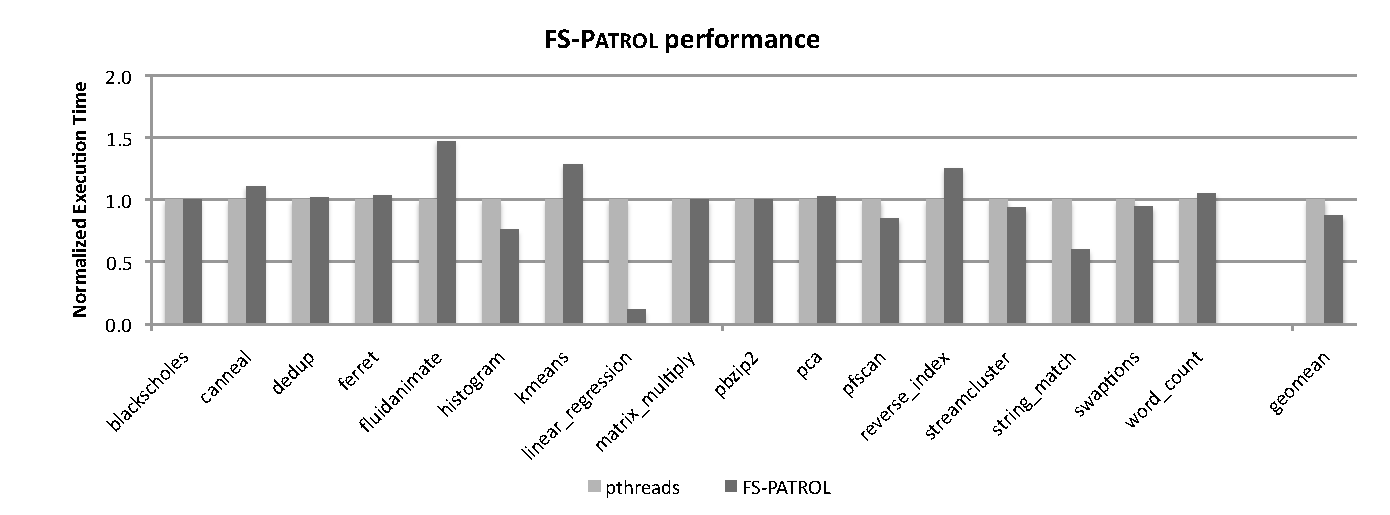
\includegraphics[width=6in]{sheriff/figure/patrolperf.pdf}
\caption{\sheriffprotect{} performance across two suites of benchmarks,
  normalized to the performance of the \pthreads{} library (see
  Section~\ref{sec:results-runtime-overhead}). In case of
  catastrophic false sharing, \sheriffdetect{} dramatically increases performance.
\label{fig:patrol}}
\end{figure*}

Here, we examine the performance improvement by tolerating the false sharing problems in
\sheriffprotect{}.
The performance improvement can be seen in the Figure~\ref{fig:patrol}.  

From the results, we can see that \texttt{linear\_regression} exhibits almost
a 10X speedup against the one using \pthreads{} library.  
By tolerating the serious false sharing problem inside (see
Table~\ref{table:perfafterfix}), \sheriffprotect{} achieves a significant performance 
benefit for this benchmark.
\texttt{histogram} performance benefit comes from one munmap() call to unmap about 400M's file, 
we currently are not sure about why multi-process framework can perform better in this case.

There are three benchmarks which runs at most 30\% slower than using the \pthreads{}. 
We examine the reasons to cause this slowdown. 
For \texttt{kmeans}, this application creates more than 3000 threads about 8 seconds. Since the overhead
to create one process is higher than that to create one thread, this part of 
overhead dominates most of overhead. 

For \texttt{reverse\_index} and \texttt{fluidanimate}, 
they exhibit slowdown because of the use of the processes-as-threads framework. 
This performance impact arises
from the use of a file-based mapping, which connects the private
mapping and shared mapping. The Linux page fault handler does more
work when operating on file-based pages than on anonymous pages (the
normal status of heap-allocated pages). The first write on a
file-mapped page repopulates information from the file's page table
entry. Also, the shared store for all heap pages is initially set to
\texttt{MAP\_SHARED}, so writing to one shared page can cause a
Copy-On-Write operation in the kernel even when there is only one user.
\texttt{fluidanimate} has an enormous number of transactions(18 Million), \sheriffprotect{} 
introduces some additional ovherhead for every trnasaction. That also accounts for part of
overhead.



\chapter{\Predator{}: Predictive False Sharing Detection}
This chapter presents \Predator{}, which improves the detection of false sharing. \SheriffDetect{} reports false sharing accurately and precisely with only $20\%$ performance overhead. However, it can only detect write-write false sharing for those programs using \pthreads{} library. It can also break programs that communicate across different threads with stack variables or self-defined synchronizations. These shortcomings greatly limit \Sheriff{}'s usage on real-world applications.  

In contrast to \SheriffDetect{}, \Predator{} detects all types of false sharing and has no limitations on applications. \Predator{} has been utilized to find actual false sharing in real applications, including \texttt{MySQL} and the \texttt{Boost} library.

In addition, \SheriffDetect{} and other systems share one key limitation: they can only report \emph{observed} cases of false sharing. As Nanavati et al.\ point out, false sharing is sensitive to where objects are placed in cache lines and so can be affected by a wide range of factors~\cite{OSdetection}. For example, using the gcc compiler \emph{accidentally} eliminates false sharing in the Phoenix linear\_regression benchmark at certain optimization levels, while LLVM does not do so at any optimization level.  A slightly different memory allocation sequence (or different memory allocator) can reveal or hide
false sharing, depending on where objects end up in memory; using a different hardware platform with different addressing or cache line sizes can have the same effect. All of this means that existing tools cannot root out potentially devastating cases of false sharing that could arise with different inputs, in different execution environments, and on different hardware platforms.

\Predator{} is the first system that can \emph{predict} potential false sharing that does not manifest in an execution but may appear and greatly degrade the performance of programs in a slightly different
environment. Predictive false sharing generalizes from a single execution to identify potential false sharing instances that are within one cache line of each other, which could be exposed by slight changes in object placement and alignment. It also can predict false sharing in hardware platforms with larger cache line sizes by tracking accesses within \emph{virtual cache lines} that span multiple physical lines. Predictive false sharing detection thus overcomes a key limitation of previous detection tools.

\section{False Sharing Detection}
\label{sec:detection}

We first describe \Predator{}'s false sharing detection mechanism, which consists of both compiler and runtime system
components. Section~\ref{sec:prediction} then explains how \Predator{} predicts potential false sharing based on a single execution.

\subsection{Overview}
\label{sec:overview}
False sharing only occurs when two threads
simultaneously access independent data in the same cache line.
In the remainder of this paper, we assume for the purposes of exposition that each thread runs on a 
distinct core with its own private cache.

Given this assumption, we observe that 
if a thread writes a cache line after other threads have 
accessed the same cache line, this write operation most likely causes at least a cache invalidation. Drawing from this \textbf{basic observation}, \Predator{} tracks cache invalidations of all cache lines and ranks the severity of performance degradation of any detected false sharing problems according to the number of cache invalidations. 
% by keeping track of accesses from different threads. 
 
In order to track cache invalidations, \Predator{} relies on the compiler instrumentation to track memory accesses of applications. The design tradeoff of choosing compiler instrumentation has been discussed in Section~\ref{sec:instrumentationtradeoff}. A compiler can easily identify read or write accesses. However, a compiler does not know how and when those instructions are being executed, since that depends on a specific execution, input, and runtime environment.

Therefore, \Predator{} combines a runtime system with compiler
instrumentation to track cache invalidations: the compiler
instruments memory accesses so the runtime system is notified when an access is executed (see Section~\ref{sec:compiler}), and the runtime system is responsible for collecting and analyzing actual memory accesses to detect and report false sharing (see Section~\ref{sec:runtime}).

\subsection{Compiler Instrumentation}
\label{sec:compiler}

\Predator{} relies on LLVM to perform instrumentation at the intermediate representation level~\cite{llvm}.
It traverses all functions one by one and searches for memory accesses to global and heap variables.  For each memory access, \Predator{} instruments a function call to invoke the runtime system with the memory access address and access type. \Predator{} currently omits accesses to stack variables by default because stack variables are normally used for thread local storage and therefore do not normally introduce false sharing. However, instrumentation on stack variables
can always be turned on when necessary.

The instrumentation pass is placed at the very end of the LLVM
optimization passes so that only those memory accesses surviving all previous LLVM optimization passes are instrumented.  This technique is similar to the one used by AddressSanitizer~\cite{AddressSanitizer}.

\subsection{Runtime System}
\label{sec:runtime}

\Predator{}'s runtime system collects every memory access by handling those functions calls inserted during the compiler instrumentation phase. It analyzes possible cache invalidations based on the basic observation discussed in Section~\ref{sec:overview}. Finally, \Predator{} precisely reports any performance-degrading false sharing problems it finds.  For global variables involved in false sharing, \Predator{} reports their name, address and size; for heap
objects, \Predator{} reports the callsite stack for their allocations, their address and size. In addition, \Predator{} provides word granularity access information for those cache lines involved in false sharing, including which threads accessed which words.  This information can further help users diagnose and fix false sharing instances.

\subsubsection{Tracking Cache Invalidations}
\Predator{} only reports those global variables or heap objects on cache lines with a large number of cache invalidations. It is critical to track cache invalidations effectively so that \Predator{} delivers accurate reports.
\Predator{} achieves this goal by maintaining a two entry cache history table for each cache line.  In this table,
each entry has two fields: the thread ID and access type (read or write). The thread ID is used to identify the origin of each access. As stated earlier, only accesses from different threads can cause cache invalidations.

\begin{comment}
\begin{table}
\centering
  \begin{tabular}{ l | r }
    \hline
    {Thread ID} & {Type of Access} \\ \hline
    \hline
     &   \\ \hline
     &   \\ \hline
  \end{tabular}
  \caption{Two-entries-cache-history table for every cache line. \label{table:cachehistory}}
\end{table} 
\end{comment}

For every new access to a cache line $L$, \Predator{} checks $L$'s history table $T$ to decide whether there is a cache invalidation based on the following rules.  Note that table $T$ only has two statuses: full and not full.  There is no ``empty'' status since every cache invalidation should replace this table with the current write access.

\begin{itemize}
\item
  For a read access $R$, 
  \begin{itemize}
    \item
      If $T$ is full, there is no need to record this read access.
    \item
      If $T$ is not full and another existing entry has a different thread
      ID, then \Predator{} records this $R$ and its thread by adding a new entry to the table. 
  \end{itemize}
\item
  For a write access $W$, 
  \begin{itemize}
    \item
      If $T$ is full, then $W$ can cause a cache invalidation since at least one of two existing entries has a different thread ID.
      After recording this invalidation, \Predator{} updates the
      existing entry with $W$ and its thread.
    \item
      If $T$ is not full,
      \Predator{} checks whether $W$ and the existing entry has the same thread ID. If
      so, $W$ cannot cause a cache invalidation, so \Predator{} updates the existing
      entry with $W$. Otherwise, \Predator{} identifies an invalidation on this line caused by $W$. 
      After recording this invalidation information, \Predator{} updates the
      existing entry with $W$ and its thread.
  \end{itemize}
\end{itemize}

\subsubsection{Reporting False Sharing}

After the cache lines with a large number of cache invalidations are detected,
\Predator{} needs further analysis to differentiate actual false sharing from true sharing. 
True sharing, e.g., multiple threads updating the same counter in a cache line, can also cause a large number of cache invalidations.

In order to report false sharing precisely and accurately,  
\Predator{} employs the following mechanisms. 

\begin{itemize}
\item

\Predator{} keeps track of access information for each word on those cache lines involved in false sharing: how many reads or writes to each word by which thread.  When a word is accessed by multiple threads, we mark the origin of this word as a shared access and do not track threads for further accesses to it. This information lets \Predator{} accurately distinguish false sharing from true sharing in the reporting phase.  It also helps diagnose where
actual false sharing occurs when there are multiple fields or multiple
objects in the same cache line, as this can greatly reduce the manual
effort required to fix the false sharing problems.

\item
In order to precisely report the origins of heap objects with false
sharing problems, \Predator{} maintains callsite information for each heap
object and reports source code level information for each heap
object. To obtain callsite information, \Predator{} intercepts all memory allocations and de-allocations, and relies
on the \texttt{backtrace()} function in the \texttt{glibc} library to obtain the whole callsite stack.
\Predator{} also avoids pseudo false sharing (false positives) caused by memory reuses because it updates recording information at memory de-allocations for those objects without false sharing problems; heap objects involved in false 
sharing are never reused.


\item
For every access, \Predator{} needs to lookup the corresponding cache line's metadata 
in order to store detailed information or update access counters. Because this operation is so frequent,
 lookups need to be very efficient.
Like 
AddressSanitizer~\cite{AddressSanitizer} and other systems~\cite{qinzhao,Valgrind},
\Predator{} uses a shadow memory mechanism to store metadata for every piece of application data. 
Thus, \Predator{} can compute and locate corresponding metadata directly via address arithmetic.

\item
In order to support shadow memory, \Predator{} uses a predefined starting address and fixed size for its heap.  It also contains a custom memory allocator, which is built with Heap Layers~\cite{heaplayers} using a ``per-thread-heap'' mechanism similar to that used by Hoard~\cite{Hoard}.  In this allocator, memory allocations from different threads never occupy the same physical cache line, which automatically avoids false sharing among different objects.  However, using this custom memory allocator implies that false sharing caused by a memory allocator cannot be detected by \Predator{}. The way to solve any such false sharing problem is to use a better allocator, since allocators like Hoard already avoid this kind of false sharing.

\end{itemize} 
 
\subsection{Optimizations}
\label{optimization}
Tracking every memory access can be extremely expensive, thus 
\Predator{} utilizes the following mechanisms to further reduce overhead.

\subsubsection{Threshold-Based Tracking Mechanism}
\label{sec:thresholdtracking}
\Predator{} aims to detect false sharing that significantly degrades performance. Since cache invalidations are the root cause of performance degradation and only writes 
can possibly introduce cache invalidations, 
cache lines with a small number of writes are never a significant performance bottleneck.
For this reason, \Predator{} only tracks cache invalidations
once the number of writes to a cache line crosses a
pre-defined threshold, which we refer to as the {\it Tracking-Threshold}. 
Before this threshold is reached, \Predator{} only tracks the number of writes on a cache line 
while skipping tracking for reads.
This mechanism reduces performance and memory overhead
at the same time.

In the current implementation, \Predator{} maintains two arrays in shadow memory: 
{\it CacheWrites} is used to track the number of memory writes on every cache line, and
{\it CacheTracking} tracks detailed information 
for each cache line once the number of writes on a cache line exceeds
the {\it Tracking-Threshold}. 
If the threshold is not reached, there is no need to check the corresponding {\it CacheTracking}. 
Figure~\ref{fig:algorithm} illustrates the detailed mechanism.

\begin{figure}[!t]
\begin{lstlisting}
void HandleAccess(unsigned long addr, bool isWrite) {
 unsigned long cacheIndex=addr>>CACHELINE_SIZE_SHIFTS;
 cachetrack *track=NULL;

 if(CacheWrites[cacheIndex]<TRACKING_THRESHOLD) {
  if(isWrite) {
   if(ATOMIC_INCR(&CacheWrites[cacheIndex]) 
      ==TRACKING_THRESHOLD-1) {
    track=allocCacheTrack();
    ATOMIC_CAS(&CacheTracking[cacheIndex],0,track));
   }
  } 
 }
 else {
  track=CacheTracking[index]);
  if(track){
   // Track cache invalidations and detailed accesses
   track->handleAccess(addr, isWrite);
  }
 }
}
\end{lstlisting}
\caption{Pseudo-code to handle an access.\label{fig:algorithm}}
\end{figure}

To avoid expensive lock operations, \Predator{} uses atomic instruction to increment 
the {\it CacheWrites} counter for each cache line. 
When the number of writes of a cache line reaches the predefined threshold,
it allocates space to track detailed cache invalidations and word accesses.
\Predator{} also 
uses an atomic compare-and-swap to set the cache tracking address for this cache line in
the shadow mapping.
After {\it CacheWrites} on a cache line reaches the {\it Tracking-Threshold}, 
all read and write accesses on this cache line are tracked.
%Cache invalidations are also computed based on cache line history table of corresponding
%cache line, shown in Table~\ref{table:cachehistory}. 


\subsubsection{Selective Compiler Instrumentation}
\label{sec:selectinstrumentation}

\Predator{} relies on instrumentation to provide memory access information to the runtime system 
and detects false sharing based on the sequences of memory accesses on every cache line. 
The performance overhead of a specific program is always proportional to 
the degree of instrumentation: more 
instrumentation means more performance overhead. 
Thus, \Predator{} provides a flexible framework to instrument programs 
depending on the performance requirements of the user.

Currently, \Predator{} only adds instrumentation once for each type of memory access on each address 
to the same basic block. 
This selective instrumentation does not normally affect the effectiveness of detection. 
Because \Predator{} aims to detect false sharing cases with a large number of cache invalidations,
less tracking of accesses inside a basic block can induce fewer cache invalidations 
but it does not affect the overall behavior of cache invalidations. 

% detection will not cause performance problem. 
To improve performance further,
\Predator{} can be easily extended to support more flexible instrumentation as follows:
\begin{itemize}
\item
\Predator{} could selectively instrument both reads and writes or only writes.
Instrumenting only writes reduces overhead while detecting write-write false sharing, 
as \Sheriff{} does. 
\item
\Predator{} can be set to instrument or skip specific code or data. 
For example, the user could provide a black-list so that given modules,
functions or variables are not instrumented. 
Conversely, the user could provide a white-list so that only specified functions or variables are instrumented. 
\end{itemize}

\subsubsection{Sampling Mechanism}
\label{sec:sample}
As described in Section~\ref{sec:thresholdtracking}, when the number of
writes on a cache line is larger than {\it Tracking-Threshold}, every
access must be tracked to store details such as word access
information, update access counter, and the cache access history table
of this cache line.  When a cache line is involved in false or true
sharing, updating those counters can exacerbate the impact of sharing
on performance: not only is there an invalidation on an application
cache line, but there is also at least another cache invalidation
caused by updating the metadata of the corresponding cache lines.

To further reduce performance overhead, \Predator{} only samples the first specified
number of accesses of each sampling interval for those problematic cache lines. 
%Note that we originally keep a global counter for all accesses and uses the number of 
%all accesses to compuate sample intervals. However, this creates 
%extereme performance overhead caused by cache invalidations of updating the same counter
%for all accesses. 
Currently, \Predator{} maintains an access counter for each cache line
and only tracks the first $10,000$ accesses out of every 1 million
accesses on a cache line (a 1\% sampling rate).



\section{False Sharing Prediction}
% Why prediction is important?
\label{sec:prediction}
This section further motivates predictive false sharing and explains how to support it in the runtime system.  

\subsection{Overview}
%\begin{figure*}[!htb]
\label{sec:predictoverview}

\begin{figure}[!t]
\begin{center}
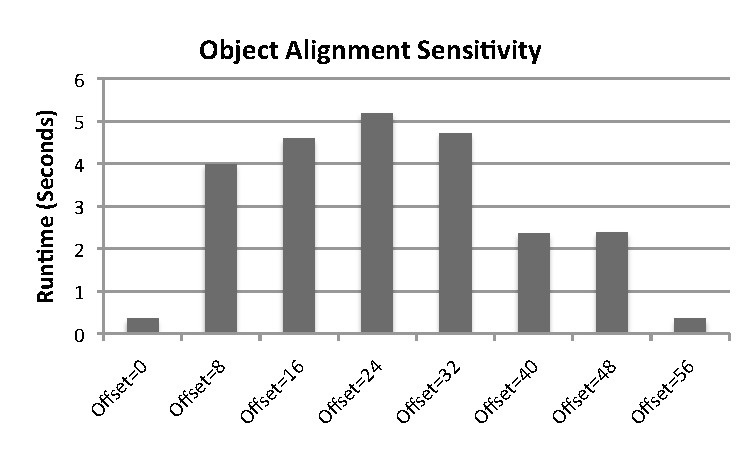
\includegraphics[width=3.3in]{predator/figure/perfsensitive}
\end{center}
\caption{
Performance of the linear\_regression benchmark from the Phoenix benchmark suite.
Performance is highly sensitive to the offset of the starting address of the (potentially) falsely-shared object 
and the start of cache line. 
\label{fig:perfsensitive}}
\end{figure}

The appearance of false sharing depends on 
the alignment between objects and corresponding cache lines.
A real example, linear\_regression, is shown in Figure~\ref{fig:perfsensitive}.
For this benchmark,
when the offset of the starting address between the potentially falsely-shared object and corresponding cache lines 
is $0$ or $56$ bytes, 
there is no false sharing. 
When the offset is $24$ bytes, we see the most severe performance effect caused 
by false sharing. 
The performance difference between these two scenarios can be as large as $15\times$. 
Existing detection tools can only report observed false sharing.
For this case, they may miss a very severe false sharing problem that could occur in the wild if the offset of the starting 
address was $0$ bytes or $56$ bytes in their test environment.
\Predator{} overcomes this shortcoming by accurately predicting potential false sharing.

\begin{figure*}
\begin{center} 
\subfigure[No false sharing]{%
   \label{fig:nofs}
   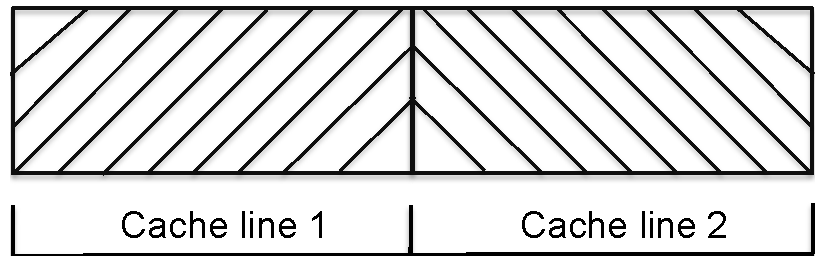
\includegraphics[width=0.24\textwidth]{predator/figure/Potential1}
}%
\hspace{30pt}
\subfigure[False sharing with larger cache size]{%
   \label{fig:fslarger}
   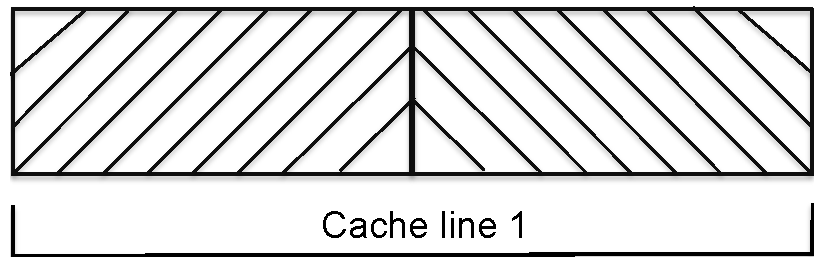
\includegraphics[width=0.24\textwidth]{predator/figure/Potential2}
}%
\hspace{30pt}
\subfigure[False sharing with different alignment]{%
   \label{fig:fsnoalignment}
   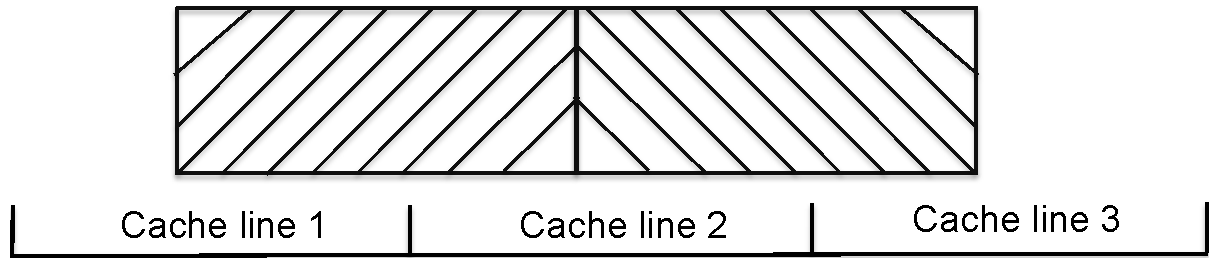
\includegraphics[width=0.36\textwidth]{predator/figure/Potential3}
}%
\end{center}
%\includegraphics{fig/potential.pdf}
\caption{False sharing under different environments.}
\label{fig:potentialfalsesharing}
\end{figure*}

\Predator{} predicts {\it potential false sharing}, the type of
false sharing that does not 
manifest in the current execution but may appear and greatly affect programs' performance
in a slightly different environment.

Figure~\ref{fig:potentialfalsesharing} shows a simplified example why occurrences of false sharing 
can change in different situations.
In this figure, two rectangles with different patterns
represents two portions of the same object, updated by different threads. 
In Figure~\ref{fig:nofs}), there is no false sharing when thread T1 only updates 
``cache line 1'' and T2 only updates ``cache line 2''.
However, false sharing appears in one of the following cases, even with the same
access pattern. 

\begin{itemize}
\item
Doubling cache line size (Figure~\ref{fig:fslarger}). When the size of a
cache line doubles,
both T1 and T2 access the same cache line and false sharing occurs in this case.

\item
Different starting address of an object(Figure~\ref{fig:fsnoalignment}). 
When the starting address of this object is not aligned with the starting address of 
the first cache line, 
then T1 and T2 can update the second cache line simultaneously, 
causing false sharing. 
%When some dynamic property changes the starting address of this object so that it 
%is not aligned with the starting address of the first cache line, 
\end{itemize} 

\Predator{} predicts whether programs can have potential false sharing  
in either of these two cases, where they can be caused by different dynamic properties 
discussed in Section~\ref{sec:intro}.
All dynamic properties, except the change of cache line size,
can lead to different starting address of an object. 
Thus, predicting false sharing in these two cases actually 
explores many possibilities caused by all dynamic properties.

\subsection{Basic Prediction Workflow}
\label{sec:predictionmechanism} 

%Similar to the detection part, 
\Predator{} focuses exclusively on potential false sharing that can 
cause performance problems.
The implementation is based on
two key observations. First, only accesses to 
adjacent cache lines can form potential false sharing, 
i.e., introducing cache invalidations when cache line size
or an object's starting address changes.
Second, only when false sharing introduces a large number of cache invalidations
can it degrade performance.

Based on these two observations, \Predator{} develops 
the following workflow to capture potential false sharing.
Those detection optimizations listed in Section~\ref{optimization} can also be applied
to prediction part. We do not repeat these optimizations in this section.

\begin{enumerate}
\item
Track the number of writes on different cache lines. 

\item
When the number of writes to a cache line $L$ reaches {\it Tracking-Threshold},
track the detailed read and write accesses for every word on both cache line $L$ 
and its adjacent cache lines. 

\item
When the number of writes to a cache line $L$ reaches a second threshold (called as
{\it Predicting-Threshold}), 
identify whether there exists false sharing in $L$ and its adjacent 
cache lines by analyzing word accesses information collected in Step 2. 
Section ~\ref{sec:evaluatingfs} describes the evaluation method.

\item
If a potential false sharing is found, continue to track cache line invalidations to confirm it. Section~\ref{sec:tracking} discusses the details.
Otherwise, go back to Step 2 to track more detailed accesses.
 
\end{enumerate}

\subsection{Searching for Potential False Sharing}
\label{sec:evaluatingfs}
To describe potential false sharing in two different cases, we first 
introduce the concept of a virtual cache line.  A virtual cache line
is a contiguous memory range that spans one or more physical cache 
lines.  In the case of double cache line size, a virtual line is
composed of two original contiguous cache lines and the first cache
line has an even index number.  Thus, only cache lines $2*i$ and
$2*i+1$ can form a virtual line.  In the case of different starting
addresses, a virtual line can have the same size as physical lines,
but can be positioned arbitrarily: unlike actual cache lines, the
starting address of a virtual cache line does not need to be multiple
of the cache line size.  For instance, a 64-byte long virtual line can
consist of the range $[0,64)$ bytes or $[8,72)$ bytes.

To search for potential false sharing problems, 
\Predator{} searches for a hot access pair on $L$ and its adjacent cache lines 
by analyzing the detailed word access information collected in Step 2. 
A hot access in a cache line refers to the word whose number of read or write accesses 
is larger than the average number of accesses to each word of cache line $L$.
For every hot access $X$ in cache line $L$, \Predator{} searches another
hot access $Y$ in $L$'s previous cache line or next cache line satisfying
the following conditions: 

\begin{itemize}
\item
$X$ and $Y$ reside on the same virtual line. 

\item
One of $X$ and $Y$ is a write access.

\item 
$X$ and $Y$ are issued by different threads.

\end{itemize}

% why it finds a pair of $X$ and $Y$ == a potential false sharing 
Whenever it finds such a pair $X$ and $Y$, 
\Predator{} identifies potential performance-degrading false sharing whenever
 the number of cache invalidations caused by $X$ and $Y$, at a possible virtual line, 
is larger than the average number of accesses on each word of $L$. 
This approach is based on a similar observation as in detection:
\emph{if a thread writes a virtual line after other threads 
have accessed the same virtual line, this write operation most likely causes at least one cache 
invalidation}. 
Before tracking detailed memory accesses on a virtual line, it is impossible to know exactly how many cache invalidations happen on a virtual line. Thus, \Predator{} conservatively assumes that accesses from different threads occurs interleavedly.
This approach ensures that \Predator{} does not miss any potential false sharing as well as 
not reporting false positives. 

%According to above observation and assumption, 
%a pair of hot accesses, $X$ and $Y$, if accesses are issued in an interleaving 
%way, can generate the number of cache invalidations equaling to 
%the smaller number of accesses of $X$ and $Y$.
%Thus a false sharing problem is to be identified by \Predator{}.
  
After identifying possible false sharing, \Predator{} goes to Step 4 to 
verify whether this is an actual false sharing problem.

\subsection{Verifying Potential False Sharing}
\label{sec:tracking}

\Predator{} verifies potential false sharing by tracking 
cache invalidations on a problematic virtual line.
%covering a pair of hot accesses found
%in Step 3.

For potential false sharing caused by double cache line size, as described in
Section~\ref{sec:evaluatingfs}, a virtual line is always composed of 
cache line with index $2*i$ and $2*i+1$. 
\Predator{} tracks cache invalidations
on the virtual line on which false sharing has been discovered.

However, for the case of a change in starting address,
two hot accesses with distance less than cache line size 
can form multiple virtual lines. 
There is thus an additional step to determine which virtual line to be tracked.
Although the virtual line to be chosen here is never a real cache line of actual hardware
because of unaligned addresses,
we utilize this virtual line to simulate the effect of changing the 
starting addresses of objects.


\begin{figure}
\begin{center} 
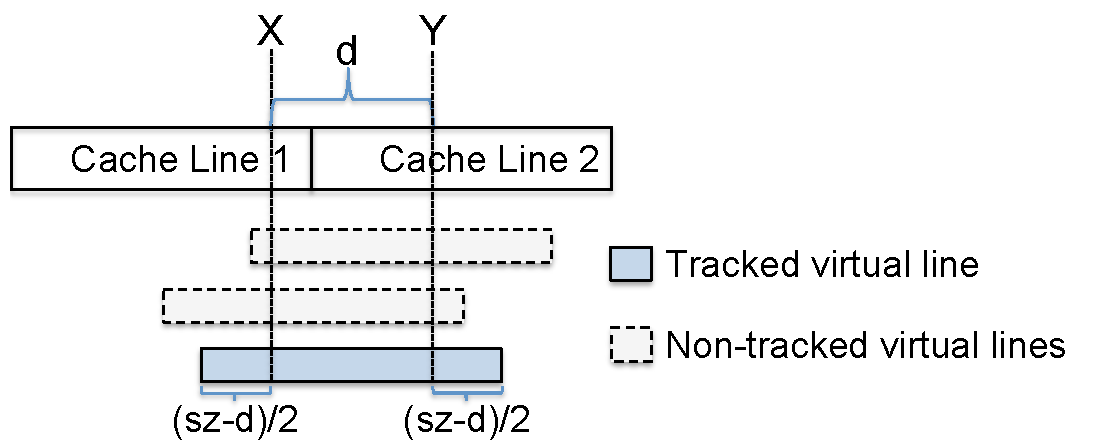
\includegraphics[width=3.3in]{predator/figure/trackpotential}
\end{center}
\caption{Determining a virtual line with size $sz$ according to hot accesses.}
\label{fig:trackpotential}
\end{figure}

Given two words with the hot accesses shown in Figure~\ref{fig:trackpotential}, 
\Predator{} leaves the same space before $X$ and after $Y$ in determining a virtual line. 
That is, the virtual line starting 
at location $X-((sz-d)/2)$ and ending at $Y+((sz-d)/2)$ is tracked. 
This choice allows tracking of more possible cache invalidations caused by
adjacent accesses of $X$ and $Y$. 
Since adjusting the starting address of a virtual line has the same effect of
adjusting the starting address of an object in detecting false sharing,
all cache lines related to the same object must be adjusted at the same time.
\Predator{} then tracks cache invalidations based on these adjusted virtual lines.



\section{Evaluation}
\begin{figure*}[htb]
{\centering
\tiny
\subfigure{\lstinputlisting[numbers=none,frame=none,boxpos=t]{predator/figure/linearregression.report}}
\caption{An example report by \Predator{} indicating false sharing in the linear\_regression benchmark.
\label{fig:lrreport}}
}
\end{figure*}



\label{sec:evaluation}

This section answers the following questions:
\begin{itemize}
\item
  How effective is \Predator{} at detecting and predicting false sharing?

\item
  What is \Predator{}'s overhead, in terms of execution time and memory ?

\item
  How sensitive is \Predator{} to different sampling rates?
 
\end{itemize}

\paragraph{Experimental Platform.} All evaluations are performed on a quiescent Intel Core 2 dual-processor system equipped with 
16GB RAM. Each processor is a 4-core 64-bit Intel Xeon running at 2.33 GHz, with a 4MB shared L2 cache and 32KB private L1 cache. The underlying operating system is an unmodified CentOS 5.5, running with Linux kernel version 2.6.18-194.17.1.el5. The glibc version is 2.5. 

\paragraph{Evaluated Applications.}
This paper evaluates two popular benchmark suites,
Phoenix (with large input) ~\cite{phoenix-hpca} and PARSEC (with simlarge input) ~\cite{parsec}. Even with unmodified LLVM-3.2, Facesim cannot be compiled successfully (having complaints on an undefined template) and Canneal aborts unexpectedly. Thus, these two benchmarks are excluded.
We also evaluate \Predator{} on six real applications, including MySQL, Boost, Memcached, aget, pbzip2 and pfscan.



\subsection{Detection and Prediction Effectiveness}
\label{sec:effective}

For every false sharing problem, \Predator{} reports source code information and detailed memory access information in order to help users fix those problems. Figure~\ref{fig:lrreport} shows an example for the linear\_regression benchmark. This report shows that the heap object starting with $0x40000038$ potentially causes a large number of cache invalidations. The call stack of allocation is provided to help locate culprits. In addition, \Predator{} also reports word-level access information of this object, which helps to identify where and how false sharing occurs. From that, we can know that it is a latent false sharing problem predicted by \Predator{}, since different threads are accessing different cache lines. 

\subsubsection{Benchmarks}
\label{sec:benchmarks}

\begin{table*}[!t]
{\centering\begin{tabular}{l|r|r|r|r|r}\hline
{\bf \small Benchmark} & {\bf \small Source Code} & {\bf \small New} & {\bf \small Without Prediction} &{\bf \small With Prediction} & {\bf \small Improvement} \\
\hline
\small \textbf{histogram} & {\small histogram-pthread.c:213} & \cmark{} &\cmark{} & \cmark{} & 46.22\%\\
\small \textbf{linear\_regression} & {\small linear\_regression-pthread.c:133} & & & \cmark{} & 1206.93\% \\
\small \textbf{reverse\_index} & {\small reverseindex-pthread.c:511} & & \cmark{} & \cmark{} & 0.09\%\\
\small \textbf{word\_count} & {\small word\_count-pthread.c:136} & & \cmark{} & \cmark{} & 0.14\%\\
\hline
\small \textbf{streamcluster} & {\small streamcluster.cpp:985} &  & \cmark{} & \cmark{} &7.52\% \\
\small \textbf{streamcluster} & {\small streamcluster.cpp:1907} & \cmark{} & \cmark{} & \cmark{} & 4.77\%\\
\hline
\end{tabular}
\caption{False sharing problems in the Phoenix and PARSEC benchmark suites. \label{table:detection}}
}
\end{table*}

Table~\ref{table:detection} provides detection results of two benchmark suites, Phoenix and PARSEC
The first column lists those programs with false sharing problems.  The second column shows precisely where the problem is. Because all discovered false sharing occurs inside heap objects, we show callsite source code information here.  The third column, ``New'', marks whether this false sharing was newly discovered by \Predator{}.  A checkmark in the following two columns indicates whether the false sharing was identified without
prediction and/or with prediction.  The final column, ``Improvement'', shows the performance improvement after fixing false sharing.
%The number is based on the average runtime of $10$ runs. 

As shown in the table, \Predator{} reveals two unknown false sharing problems. It is the first tool to detect the false sharing problems in histogram and in line $1908$ of streamcluster. 
In histogram, multiple threads simultaneously modify different locations of the same heap object, thread\_arg\_t. 
Padding this data structure fixes the false sharing problem and improves the performance by around 46\%. In streamcluster, multiple threads are simultaneously accessing and updating the same \texttt{bool} array, switch\_membership. Simply changing all elements of this array to a long type reduces the false sharing and improves the performance by about 4.7\%.

%, although it is not a complete fix of false sharing. 
%None of these two false sharing problems has been reported by previous tools.
Other false sharing problems were discovered by previous work~\cite{sheriff}. We do not see significant performance improvement for reverse\_index and word\_count benchmarks. They are reported here because the number of cache invalidations in these two programs reaches our predefined threshold.
Making the reporting threshold higher can avoid the report of those insignificant false sharing problems.
It is worth noting that these two benchmarks definitely have false sharing problems,
which can be confirmed by word-level information generated by \Predator{}. 

The streamcluster benchmark has another false sharing problem at line $985$. Different threads change the work\_mem object simultaneously. Authors of streamclsuter have already realized this problem and provide a CACHE\_LINE macro. Unfortunately, the default value of this macro is set to $32$ bytes, which is different from the actual cache line size of the experimental machine. By setting it to $64$ bytes instead, it achieves  performance improvement of about 7.5\%.

linear\_regression has a severe false sharing problem. Fixing it improves the performance by more than $12\times$. In this benchmark, different threads update their thread-specific locations inside the tid\_args object in a tight loop. According to the observation of Nanavati et al., this false sharing problem occurs when using clang and disappears when using gcc with the -O2 and -O3 optimization level~\cite{OSdetection}. But we observed a different result when using the clang-3.2 compiler and our custom memory allocator: the false sharing problem does not occur at all because the offset of the starting address of the potentially falsely-shared object and the start of cache line is 56 bytes (see Figure~\ref{fig:perfsensitive}). With prediction mechanism, \Predator{} detects this latent false sharing problem, exemplifying the necessity of a predictive detection tool. 

\subsubsection{Real Applications}
To verify \Predator{}'s practicality, we further evaluate several widely-used real applications, whereas no previous work has done this. These real applications include a server application (MySQL~\cite{mysql}),
a standard C++ library (Boost~\cite{libfalsesharing}),
a distributed memory object caching system (Memcached), a network retriever (aget),
a parallel bzip2 file compressor (pbzip2), and a parallel file scanner (pfscan).

MySQL-5.5.32 and boost-1.49.0 are known to have false sharing problems. Other applications (memcached-1.4.15, aget-0.4.1 and pbzip2-1.1.6) do not have known false sharing problems.

The false sharing of MySQL has caused a significant scalability problem and was very difficult to identify.
According to the architect of MySQL, Mikael Ronstrom, ``we had gathered specialists on InnoDB..., participants from MySQL support... and a number of generic specialists on 
computer performance...'', ``[we] were able to improve MySQL performance by 6$\times$ with those scalability fixes''~\cite{mysql}. 
The false sharing inside Boost is caused by the usage of a  spinlock pool. Different threads may utilize different spinlocks located in the same cache line in this case. Fixing it brings a 40\% performance improvement.
\Predator{} is able to pinpoint false sharing locations in both MySQL and the Boost library. 
For the other four applications, \Predator{} does not find severe false sharing problems.

\subsubsection{Prediction Effectiveness}
\label{sec:predicteval}
In this section, we verify whether prediction can always  reveal un-observed false sharing problems.

The linear\_regression benchmark is selected here because of the following two reasons: (1) The false sharing problem of this benchmark cannot be detected without prediction; (2) False sharing severely degrades performance when it actually occurs. Hence, it is a serious problem that should always be detected. 

\begin{figure}[!t]
{\centering
\subfigure{\lstinputlisting[numbers=none,frame=none,boxpos=t]{predator/figure/linearregression.psedocode}}
\caption{The false sharing problem inside the linear\_regression benchmark: multiple threads simultaneously update their entries in lreg\_args.
\label{fig:linearregression}}
}
\end{figure}

Figure~\ref{fig:linearregression} shows the data structure and the source code exercising appropriate false sharing. The size of this data structure, lreg\_args, is $64$ bytes 
when the program is compiled to a $64$-bit binary. For this benchmark, the main thread allocates an array, containing as many elements as the number of underlying hardware cores. Each element is a lreg\_args type with $64$ bytes. This array is then passed to different threads (lreg\_thread function) so that each thread only updates its thread-dependent area. False sharing occurs if two threads happen to update data in the same cache line. 

Figure~\ref{fig:perfsensitive} shows how sensitive the performance is to different starting addresses of a falsely-shared object. When the offset is $0$ or $56$ bytes, this benchmark achieves its optimal performance and has no false sharing. When the offset is $24$ bytes, the benchmark runs around $15$ times slower than its optimal performance because of the false sharing problem.

Our evaluation shows that \Predator{} can always detect the false sharing problem with prediction enabled, demonstrating its effectiveness.

\subsection{Performance Overhead}
\label{sec:perfoverhead}

\begin{figure*}[!t]
\centering
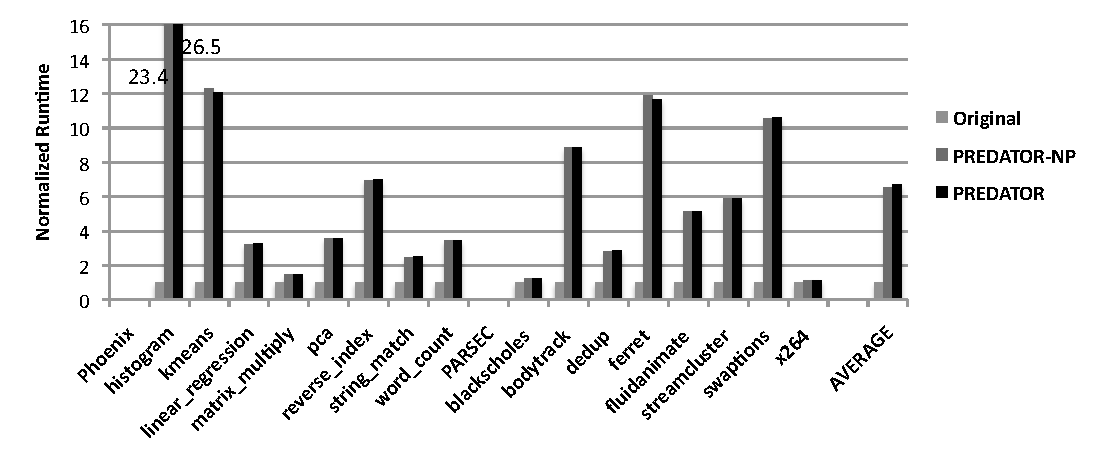
\includegraphics[width=6in]{predator/figure/perf}
\caption{
Performance overhead of \Predator{} with and without prediction(PREDATOR-NP).
\label{fig:perf}}
\end{figure*}

To avoid the effect caused by extreme outliers, all performance data shown in Figure~\ref{fig:perf} is based on the average of $10$ runs, excluding the maximum and minimum values. 

For $16$ benchmarks from the Phoenix and PARSEC benchmark suites and six real applications, \Predator{} imposes $5.4\times$ performance overhead. There is no noticeable difference on performance whether the prediction mechanism is enabled or not. 
 
Among these programs, five of them, histogram, kmeans, bodytrack, ferret, and swaptions, have more than $8\times$ performance overhead. The histogram benchmark runs more than $26\times$ slower than original executions with \pthreads{} library, because tracking detailed access on cache lines with false sharing exacerbates the false sharing effect (see more discussion in Section~\ref{sec:sample}).  For bodytrack and ferret, although there is no false sharing, \Predator{} detects a large amount of cache lines with writes larger than {\it Tracking-Threshold}. Thus, tracking those accessing details for those cache lines imposes significant performance overhead. Currently, we cannot identify the reasons why kmeans runs very slowly on \Predator{}.
   
\Predator{} imposes a small performance overhead for IO-bound applications, such as matrix\_multiply, blackscholes, x264, aget, Memcached, pbzip2, and pfscan, since \Predator{} does not add any performance overhead for IO operations.  

\subsection{Memory Overhead}
\label{sec:memoverhead}
We only evaluate the physical memory overhead of \Predator{}, instead of the virtual memory overhead, because \Predator{} allocates four gigabytes virtual memory for its custom memory allocator. Proportional set size (PSS) in \texttt{/proc/self/smaps} reflects the physical memory increase on the existing system of running an application~\cite{memusage}. Thus, we periodically collect this data and use the sum of different memory mappings as the total physical memory usage of running an application. We present the maximum value of physical memory usage in Figure~\ref{fig:memusage}. 

\Predator{} imposes less than 50\% memory overhead for 17 out of 22 applications.  For swaptions and aget, \Predator{} introduces more memory overhead because the original memory footprints of them are very small, only $3$ kilobytes. Adding the code of detection, prediction and reporting contributes to a large ratio of memory overhead. We are not clear why MySQL consumes much more memory than others. Although the average memory usage of all applications is over $2\times$, the total memory usage overhead is only about $40\%$ on \Predator{}. 


\subsection{Sensitivity to Different Sampling Rates}
\label{sec:sensitivity}
In Section~\ref{sec:sample}, we discuss that \Predator{} utilizes the sampling mechanism to reduce the tracking overhead. Running an application with different sampling rates does not affect its memory usage. Thus, we only evaluate the effect of different sampling rates on performance and effectiveness. 

The default sampling rate used by \Predator{} is 1\%. In this section, we also evaluate two other sampling rates, 0.1\% and 10\%. The performance results under the three different sample rates are shown in Figure~\ref{predator/figure:sample}. \Predator{} introduces less performance overhead under a lower sampling rate, which meets our expectation. Concerning effectiveness, even using the 0.1\% sampling rate, \Predator{} can still detect all false sharing problems, but with a lower number of cache invalidations. Thus, different sampling rates do not affect the detection effectiveness.
 
\begin{figure*}[!t]
\centering
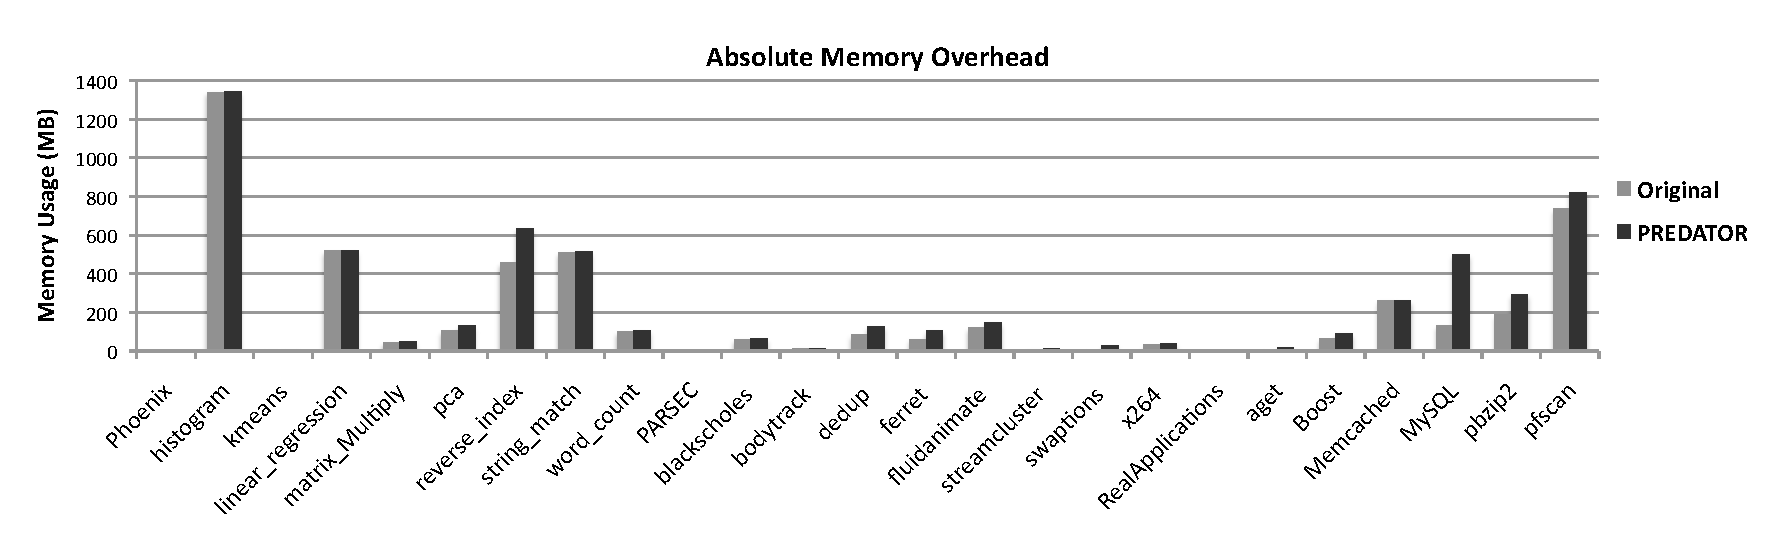
\includegraphics[width=6in]{predator/figure/absolutememory}
\caption{Absolute physical memory usage overhead with \Predator{}.}
\label{fig:absolutememusage}
\end{figure*}

\begin{figure*}[!t]
\centering
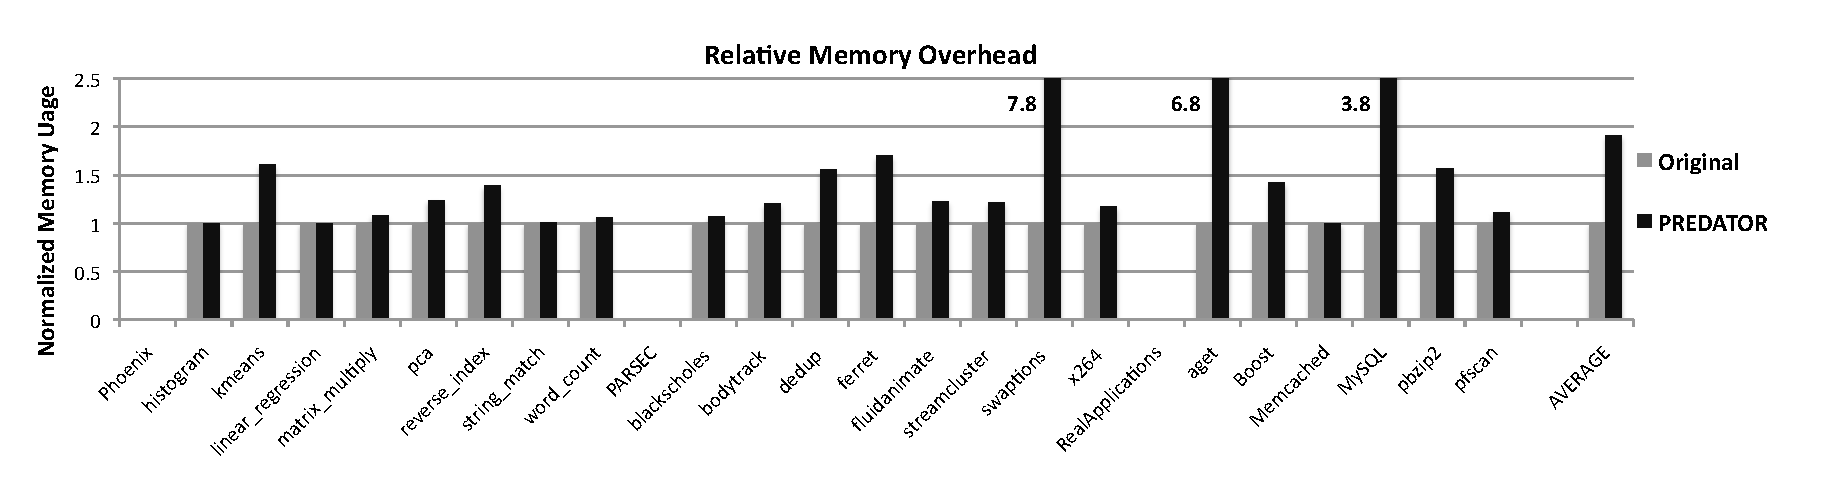
\includegraphics[width=6in]{predator/figure/memusage}
\caption{Relative physical memory usage overhead with \Predator{}.}
\label{fig:memusage}
\end{figure*}






\chapter{Related Work}

\label{chapter:relatedwork}
This chapter first describes those related work to processes-as-threads framework and deterministic execution. Then it describes related work in false sharing detection, prevention, or both. 

\section{Processes-As-Threads framework}

BOP relies on strong isolation of processes to automatically and safely parallelize the execution of programs~\cite{DingBOP}. BOP forks a new process to do speculation, based on those pre-defined possibly parallel regions (PPR). In order to check the correctness, BOP tracks accesses on a page-based granularity. When there is no conflict and a speculative process reaches the end of its current PPR, its predecessor always commits its changes to the current process. However, BOP does not provide any synchronization support and can not be used to run normal multithreaded programs. 

Grace is a process-based approach designed to prevent
concurrency errors, such as deadlock, race conditions, and
atomicity errors by imposing a sequential semantics on
speculatively-executed threads~\cite{grace}. Grace supports only fork-join programs without inter-thread communication (e.g., condition variables or barriers), and rolls back threads when accesses of threads would violate sequential semantics: a thread accesses pages that have been accessed by its predecessors. Grace can not support arbitrary multithreaded programs. Similar to the Grace system, Sammati is a processes-as-threads system to detect and tolerate deadlock problems~\cite{Pyla:2010:ADA:1854273.1854288}. However, Sammati does not support the full range of synchronizations, without synchronizations, barriers, and signals. Also, Semmati can not avoid race conditions happening in creating twin pages, which are avoided by \Sheriff{} framework.

\begin{comment}
% Some usage of this framework
According to Revisions,  Grace cannot easily resolve all
conflicts on commit (like revisions do) and must thus restrict
tasks from producing such conflicts either statically (by type
system) or dynamically (pessimistic with blocking, or optimistic with abort and retry). Also, Grace allows only a restricted “fork-join” form of concurrency
Revisions~\ref{Burckhardt:2010:CPR:1869459.1869515}
\end{comment}

\section{Deterministic Multithreading}
The research on deterministic multithreading is a very active area these years. We describe some software-only, non- language-based approaches here.

\subsection{Software-only deterministic system}
Grace prevents deadlocks, race conditions, ordering and atomicity violations errors for those fork-join multithreaded programs by imposing a sequential semantics at join points~\cite{grace}. However, Grace does not support programs with interthread communications, such as conditional variables and barriers.

CoreDet is a compiler-based approach to 
support general-purpose multithreaded programs~\cite{Bergan:2010:CCR:1736020.1736029}. 
CoreDet instruments those memory read and write operations as long
as those operations can not be proved to be thread-local in static analysis. 
In the runtime phase, CoreDet divides the execution into 
alternating parallel and serial phases and guides all memory operations 
using a memory ownership table: only those owned locations can be accessed
in the parallel phases; all non-owned locations and synchronizations can only 
be accessed in the serial phases guided by a global token.
CoreDet guarantees deterministic execution for racy programs without memory errors,
but with very high performance overhead: 
averagely $3.5\times$ slower than those using \pthreads{} library.
In order to guarantee determinsim, 
CoreDet has to serialize \emph{all} external library calls without instrumentation.
CoreDet doesn not provide deterministic 
memory allocations, which can not guarantee determinism for programs with memory errors.  
% The use of synchronization points as commit boundaries also makes \dthreads{}
% code relatively \emph{robust}: when updates occur after a given number of 
% instructions retired (as in CoreDet and Kendo), it is impossible for 
% programmers to know when interleavings can occur. Such boundaries could vary 
% depending on the underlying architecture and would also be input-dependent, 
% meaning that slightly different inputs could lead to dramatically different
% thread interleavings. By contrast, \dthreads{} guarantees that only changes to
% the sequence of synchronization operations affect the order in which updates 
% are applied.
dOS~\cite{deterministic-process-groups} is an extension to CoreDet
that uses the same deterministic scheduling framework.  dOS 
supports deterministic communication for those threads and processes inside the same
deterministic process groups (DPGs) and handle those external non-determinism by recording and
replaying interactions across DPG boundaries. 

Determinator is a microkernel-based operating system that enforces
system-wide determinism~\cite{efficient-system-enforced}.
Determinator provides separate address spaces and supports interprocess
communications at explicit synchronizaton points. 
Determinator is a proof-of-concept system, which can not support the whole rage of
threads APIs and can not work on legacy programs.  

Some other works can only support limited determinism or need user annotation.
Kendo can only guarantee the determinism for race-free programs~\cite{1508256}. 
TERN~\cite{stable-deterministic} provides a best-effort system to 
apply memoized schedules for future runs with similar inputs. 
It can not guarantee the determinism for racy programs, as Kendo. 
Peregrine~\cite{peregrine:sosp11} is a system based on TERN, which tries to record
 memory accesses orders for racy portion and apply those schedules for future runs possibly.
However, both TERN and Peregrine do not support complete determinism (using a best effort)
and requires program annotations. 

\subsection{Hardware-related deterministic System}

\section{False Sharing}

This section describes related work in false sharing detection, prevention, or both. There is no previous
system to predict unobserved false sharing.

\subsection{False Sharing Detection}
Based on the SIMICS functional simulator, Schindewolf et al.\ designed a tool to report different kinds of cache usage information, such as cache misses and cache invalidations~\cite{falseshare:simulator}. Pluto relies on Valgrind dynamic instrumentation framework to track the sequence of memory read and write events on different threads, and reports a worst-case estimation of possible false sharing~\cite{falseshare:binaryinstrumentation1}.
Similarly, Liu uses Pin to collect memory access information, and reports total cache miss information~\cite{falseshare:binaryinstrumentation2}.
These tools impose about $100-200\times$ performance overhead.

Zhao et al.\ developed a tool based on DynamoRIO framework to detect false sharing and other cache contention problems
for multithreading programs~\cite{qinzhao}. 
It uses a shadow memory technique to maintain memory access history and detects cache invalidations based on the ownership of cache lines. However, it can only support at most $8$ threads. In addition, it cannot differentiate cold cache misses from actual false sharing problems.

Intel's performance tuning utility (PTU) uses Precise Event Based Sampling (PEBS) hardware support to detect false sharing problems ~\cite{detect:ptu, detect:intel}.  PTU cannot distinguish true sharing from false sharing. In addition, PTU aggregates memory accesses without considering memory reuses and access interleaving, leading to numerous false positives. Sanath et al. designed a machine learning based approach to detect false sharing problems. They train their classifier on mini-programs and apply this classifier to general programs ~\cite{mldetect}. Instead of instrumenting memory accesses, this tool relies on hardware performance counters to collect memory accesses events. It achieves very low performance overhead(about 2\%). But it relies on hardware support for its efficiency.  

In addition to their individual disadvantages,
all approaches discussed above share a common shortcoming:  
they cannot pinpoint the exact location of false sharing in the source code, so programmers have to examine the source code and identify problems manually.

Pesterev et al.\ present DProf, a tool that help programmers identify cache misses based on AMD's instruction-based sampling hardware~\cite{DProf}. DProf requires manual annotation to locate data types and object fields, and cannot detect false sharing when multiple objects reside on the same cache line.

\subsection{False Sharing Prevention}
\label{sec:fspreventwork}
% More approaches
Jeremiassen and Eggers use a compiler transformation to automatically adjust the memory layout of applications through padding and alignment~\cite{falseshare:compile}. Chow et al.\ alter parallel loop scheduling in order to avoid false
sharing~\cite{falseshare:schedule}. These approaches only works for regular, array-based scientific code.

Berger et al.\ describe Hoard, a scalable memory allocator that can reduce the possibility of false sharing by making different threads use different heaps~\cite{Hoard}. Hoard cannot avoid false sharing problem in global variables or within
a single heap object: the latter appears to be the primary source of real false sharing problems.

\subsection{False Sharing Detection and Prevention}

Plastic leverages the sub-page granularity memory remapping facility provided by the Xen hypervisor to detect and tolerate false sharing automatically~\cite{OSdetection}. However, the sub-page memory remapping mechanism is not currently supported by most existing operating system, reducing its generality. In addition, Plastic cannot pinpoint the exact source of false sharing.  
In order to utilize Plastic's prevention tool, a program has to run on the Xen hypervisor, limiting the applicability of their prevention technique.



\chapter{Conclusions and Future Work}
\label{sec:conclusion}

\dthreads{} is a deterministic replacement for the \pthreads{}
library that supports general-purpose multithreaded
applications. \dthreads{} is straightforward to deploy, requiring no
source code, and operates on commodity hardware. By converting threads
into processes, \dthreads{} leverages process isolation and virtual
memory protection to track and isolate concurrent memory updates with
low overhead. By committing these changes deterministically at natural
synchronization points in the code, rather than at boundaries based on
hardware performance counters, \dthreads{} not only ensures full
internal determinism---eliminating data races as well as
deadlocks---but does so in a way that is portable and easy to
understand. Its software architecture prevents false sharing, a
notorious performance problem for multithreaded applications running
on multiple, cache-coherent processors. The combination of these
approaches enables \dthreads{} to match or even exceed the performance
of \pthreads{} for the majority of the benchmarks examined here,
making \dthreads{} a safe and efficient alternative to \pthreads{} for
some applications.


%%
%% Beginning of back matter
\backmatter  %% <--- mandatory

%%
%% We don't support endnotes

%%
%% A bibliography is required.
\bibliographystyle{umthesis}
\bibliography{refs}
\end{document}

%%% Local Variables: 
%%% mode: latex
%%% TeX-master: t
%%% End: 
